\documentclass{hebutthesis}



\begin{document}
\pdfbookmark[section]{生成模型研究与中国画生成}{cover}
\title{生成模型研究与中国画生成}
\author{刘鹏}
\studentID{192241}
\college{人工智能与数据科学学院}
\major{计算机科学与技术}
\supervisor{汪鹏 \qquad 副教授}
\hebutThesisTime{2023年5月22日}
\maketitle

\pdfbookmark[section]{摘要}{abstract}
\pagenumbering{Roman}
\newpage
\begin{center}
    \fontsize{18}{1}\fzxbsjt{毕业设计中文摘要}
\end{center}
\begin{tcolorbox}
\begin{center}
    \fontsize{16}{0}\heiti{\textbf{生成模型研究与中国画生成}}
\end{center}
\vspace{8mm}
\noindent
{\fontsize{16}{0}\heiti{\textbf{摘要:}}}
\vspace{2mm}

\setlength{\parindent}{24pt}
生成模型是人工智能领域的重要研究方向,研究生成模型,有助于人工智能更好地理解现实世界。
近年来,生成模型在图像或文字生成方面取得了巨大突破。
在图像领域,生成模型生成的图像质量已经可以与真实图像比肩,
在文本生成方面,ChatGPT已经可以与人们自然地交谈。

生成模型是近年来非常活跃的研究领域,对生成模型进行系统回顾总结有助于对其更好地研究。
因此,本文对近年来的主要生成模型进行了较为系统地介绍,并根据是否直接定义概率密度函数,
将生成模型分为显式密度模型和隐式密度模型。
此外,对生成模型在中国画生成上的应用进行探索,使用降噪扩散模型生成中国画。
\vspace{8mm}

\noindent\textbf{关键词}: \quad 生成模型 \quad 中国画 \quad 降噪扩散模型
% \vspace{80mm}
\end{tcolorbox}


\newpage
\begin{center}
    \fontsize{18}{1}\fzxbsjt{毕业设计外文摘要}
\end{center}
\begin{tcolorbox}
\pdfbookmark[section]{ABSTRACT}{ABSTRACT}
\begin{center}
    \fontsize{14}{0}\songti{\textbf{Generative Models Research and Chinese Painting Generation}}
\end{center}
\vspace{8mm}
\noindent
{\fontsize{16}{0}\heiti{\textbf{ABSTRACT}}}
\vspace{2mm}

\setlength{\parindent}{24pt}
Generative model is an impoertant reserach direction in the field of artificial intelligence.
The research of generative model is helpful for artificial intelligence to understand the world better.
In recent years, the generative model has made great breakthroughs in image and text generation.
In the field of image, the quality of the images generated by the generative model can already be comparable to the real image.
In terms of text generation, ChatGPT can already talk to people naturally.

Generative model is a very active research field in recent years,
Systematice review and summary of generative model is helpful to better study it.
Therefore, this paper systematically introduces the main generative models in recent years, 
and depending on whether the probability density function is directly defined,
the generated models are divided into explicit density model and implicit density model.
In addition, the application of the generative model in the generation of Chinese painting is explored, 
and the diffusion model is used to generate Chinese painting.
\vspace{8mm}

\noindent\textbf{Keywords}: Generative Models, Chinese Painting, Denoising Diffusion Model
% \vspace{28mm}
\end{tcolorbox}

\setlength{\parindent}{24pt}

% 生成模型研究与中国画生成
% Generative Models Research and Chinese Painting Generation

% 基于GAN的中国山水画生成系统设计与开发
% Design and development of Chinese landscape painting generation system based on GAN
\clearpage
\pdfbookmark[section]{\contentsname}{contents}
\tableofcontents
% \listoffigures
% \listoftables


\chapter{绪论}
\setcounter{page}{1}
\pagenumbering{arabic}



\section{研究背景与意义}
%人工智能影响生活
%生成算法在人工智能领域的地位
%中国画当前情况
%中国画生成算法研究的意义
在当今时代,人工智能技术与我们日常生活的联系逐渐紧密。
智能手机、智能家居等智能设施让我们的生活更加便利,影视作品、新闻报道中也常常出现与人工智能有关内容。
理查德·费曼曾经说过:“我无法创造我所不理解的事物”,对生成模型的研究有助于让人工智能更加“理解”现实世界。
中国画{\cite{chinesepainting}}是我国传统的绘画形式,其在内容和艺术创作上,体现了古人对自然、社会及与之相关联的政治、哲学、宗教、道德、文艺及自然等方面的认识。
使用生成模型算法进行中国画创作,有助于继承和弘扬我国优秀传统文化,让中国画在新时代焕发新的光彩。









\section{国内外研究现状}
%生成模型当前情况
%人工智能
%机器学习
%深度学习
%生成模型
%生成模型算法在中国画生成方面研究
1950年,艾伦·图灵提出著名的“图灵测试” {\cite{machinery1950computing}},给出了判定机器是否具有“智能”的试验方法,即机器是否能够模仿人类的思维方式来“生成”内容继而与人交互。
某种程度上来说,人工智能从那时起就被给寄予了用于内容创造的期许{\cite{aigcwhitebook}}。
最初,人们尝试通过编码,将具体的规则赋予人工智能,但面临的各种困难使人们转变策略。
不再是直接提供人为设定的规则,而是为人工智能提供数据资料,让人工智能从数据资料中“学习”所需的规则,也就是“机器学习” {\cite{goodfellow2016deep}}。
随着计算机运算能力的增加与数据量的增长,在机器学习中,让计算模型通过多个中间层来逐渐理解数据潜在表示的“深度学习” {\cite{lecun2015deep}},逐渐在计算机视觉、自然语言处理、语音识别等领域取得了突破。

深度学习与生成模型的结合,让人工智能生成内容迎来了新时代,生成内容百花齐放,效果逐渐逼真直至人类难以分辨。

\subsection{2014--2017 变分自编码器和生成对抗网络时代}
2013年,变分自编码器 {\cite{kingma2013auto}}的提出使人们认识到,生成模型不仅可以生成简单的数字图像,还可以生成像人脸一样更复杂的图像。生成的图像可以随着隐空间取值的变化而变化。
2014年,生成对抗模型 {\cite{goodfellow2020generative}}的提出,为人们提供了一种通过对抗结构来解决生成模型问题的全新思路。
在随后三年内,人们对生成对抗网络进行了扩展与改进,
如对基础模型结构进行改进的DCGAN {\cite{radford2015unsupervised}},
对损失函数进行改进的Wassertein GAN {\cite{arjovsky2017wasserstein}},
对训练过程进行改进的ProGAN {\cite{karras2017progressive}},
还有使用生成对抗网络在新的领域进行应用,如图像与图像的转化 {\cite{isola2017image}\cite{zhu2017unpaired}}以及音乐的生成 {\cite{dong2018musegan}}。

在同时期,变分自编码器也有了一些重要的改进,如VAE-GAN {\cite{larsen2016autoencoding}}和随后的VQ-VAE {\cite{razavi2019generating}},以及在强化学习上的应用 {\cite{ha2018world}}。

在文本生成领域,自回归模型如LSTMs和GRUs仍然是主流研究方向,相同的自回归思路也应用在图像生成领域,如PixelRNN {\cite{van2016pixel}}和PixelCNN {\cite{van2016conditional}}引入了一种新的生成图像的方式。
也有一些其他生成图像方式的尝试如RealNVP {\cite{dinh2016density}}的出现,为之后规范化流模型打下了基础。

2017年,Transformer {\cite{vaswani2017attention}}的提出使生成模型的研究转向Transformers。
\subsection{2018--2019 Transformer时代}
注意力机制是Transformer模型的核心,其使自回归模型不再需要循环层。随着只有Transformer解码器的GPT {\cite{radford2018improving}}以及只有Transformer编码器的BERT {\cite{devlin2018bert}}的提出,Transformer很快成为了研究的主流方向。
之后,越来越大的模型在很多生成文本的任务上取得了很好的效果。此外,Transformer也在音乐生成上取得了不错的效果 {\cite{huang2018music}}。

在这两年,一些重要的生成对抗网络模型的提出也巩固了其在图像生成领域的地位。
如SAGAN {\cite{zhang2019self}}和BigGAN {\cite{brock2018large}}将注意力机制引入生成对抗模型,取得了很好的效果,
StyleGAN {\cite{karras2019style}}和随后的StyleGAN2 {\cite{karras2020analyzing}}向人们展示了如何控制生成图像的风格与内容。

另一方面,基于分数的模型NCSN {\cite{song2019generative}}的提出,为扩散模型的出现打下了基础。
\subsection{2020--2023 大模型时代}
在此时期,一些模型将以往不同种类的模型混合,并在此基础上进一步改进。
如VQ-GAN {\cite{esser2021taming}}将生成对抗网络的判别器引入VQ-VAE模型结构,Vision Transformer {\cite{dosovitskiy2020image}}将Transformer应用在图像领域。
2022年,StyleGAN-XL {\cite{sauer2022stylegan}}对StyleGAN的进一步改进,使其能够在更大的数据集上生成更高分辨率的图像。

于2020年提出的两个模型——DDPM {\cite{ho2020denoising}}和DDIM {\cite{song2020denoising}},为之后的大规模图像生成模型打下基础。
在图像生成领域,突然出现的扩散模型成为了生成对抗网络的竞争对手。
扩散模型不仅可以生成高质量图像,相比于生成对抗网络也更容易训练。

在2020年同一时期,拥有1750亿参数的GPT-3 {\cite{brown2020language}}发布,其可以生成关于任何主题的文本内容。
在2022年,OpenAI在GPT-3基础上发布网页应用ChatGPT,让用户可以与ChatGPT自然地交流。

在2021年到2022年,一些在大规模语料库上训练的Transformer的变体模型也涌现而出,如微软和英伟达发布的Megatron-Turing NLG {\cite{smith2022using}},谷歌发布的LaMDA {\cite{thoppilan2022lamda}}等。

在过去两年,由于Transformer系列模型在文本生成领域的成功,以及扩散模型在图像生成领域的应用,人们开始关注多模态内容生成的研究,如使用文本生成图像。
如OpenAI在2021年发布的模型DALL.E {\cite{ramesh2021zero}},随后的GLIDE {\cite{nichol2021glide}}和DALL.E 2 {\cite{ramesh2022hierarchical}},谷歌发布的Imagen {\cite{saharia2022photorealistic}}、Parti {\cite{yu2022scaling}}和MUSE以及Stability AI发布的Stable Diffusion {\cite{rombach2022high}}等。
\section{研究内容与创新点}
%对各类生成算法进行原理探究
%使用扩散模型生成中国画
生成模型算法近年来发展较为迅速,但仍缺少资料对生成模型进行较为系统的探索与研究。
如今主流生成模型有规范化流模型、自回归模型、基于能量的模型、变分自编码器、扩散模型和生成对抗网络,
各类模型最先进的算法都可以取得很好的效果,
但生成模型为什么这样设计,其真正原理是什么,各种生成模型之间有什么关系,
理解这些问题有助于设计更好的生成模型,以达到更好的生成效果。
本文为首次对各种生成模型原理进行介绍,并将各种框架纳入同一体系的,
以有助于研究人员对生成模型进一步研究。

此外,中国画为传统艺术形式,但近年来相比于西方绘画技术的普及,中国画逐渐式微。
本文对生成模型在中国画生成方面进行探索,以期望使用人工智能技术生成高质量中国画,继承与弘扬中华传统文化。





\section{论文组织结构}

第一章首先介绍研究背景与意义,
随后介绍早期人工智能生成模型情况,
再将近年来生成模型发展分为三个阶段,
2014–2017为变分自编码器和生成对抗网络时代,
2018–2019为Transformer时代
2020–2023为大模型时代。
随后介绍研究内容与创新点与论文组织结构。

第二章首先介绍生成模型算法基本理论与生成模型用途,
再根据如何表示或近似似然函数将生成模型分为三类,
分别为可求解的显示密度模型、
近似估计的显示密度模型和隐式密度模型。
其中可求解的显示密度模型与近似估计的显示密度模型都属于显式密度模型。
如图{\ref{fig:gennerative_models}}所示,
可求解密度模型包含规范化流模型和自回归模型,
近似估计密度模型包含基于能量的模型、变分自编码器和扩散模型。
{\ref{section:explicit_density_model}}对各显式密度模型进行了详细介绍,
{\ref{section:implicit_density_model}}对隐式密度模型生成对抗网络进行了详细介绍,
最后,介绍了生成模型评价方法。
\begin{figure}[ht]
    \centering
    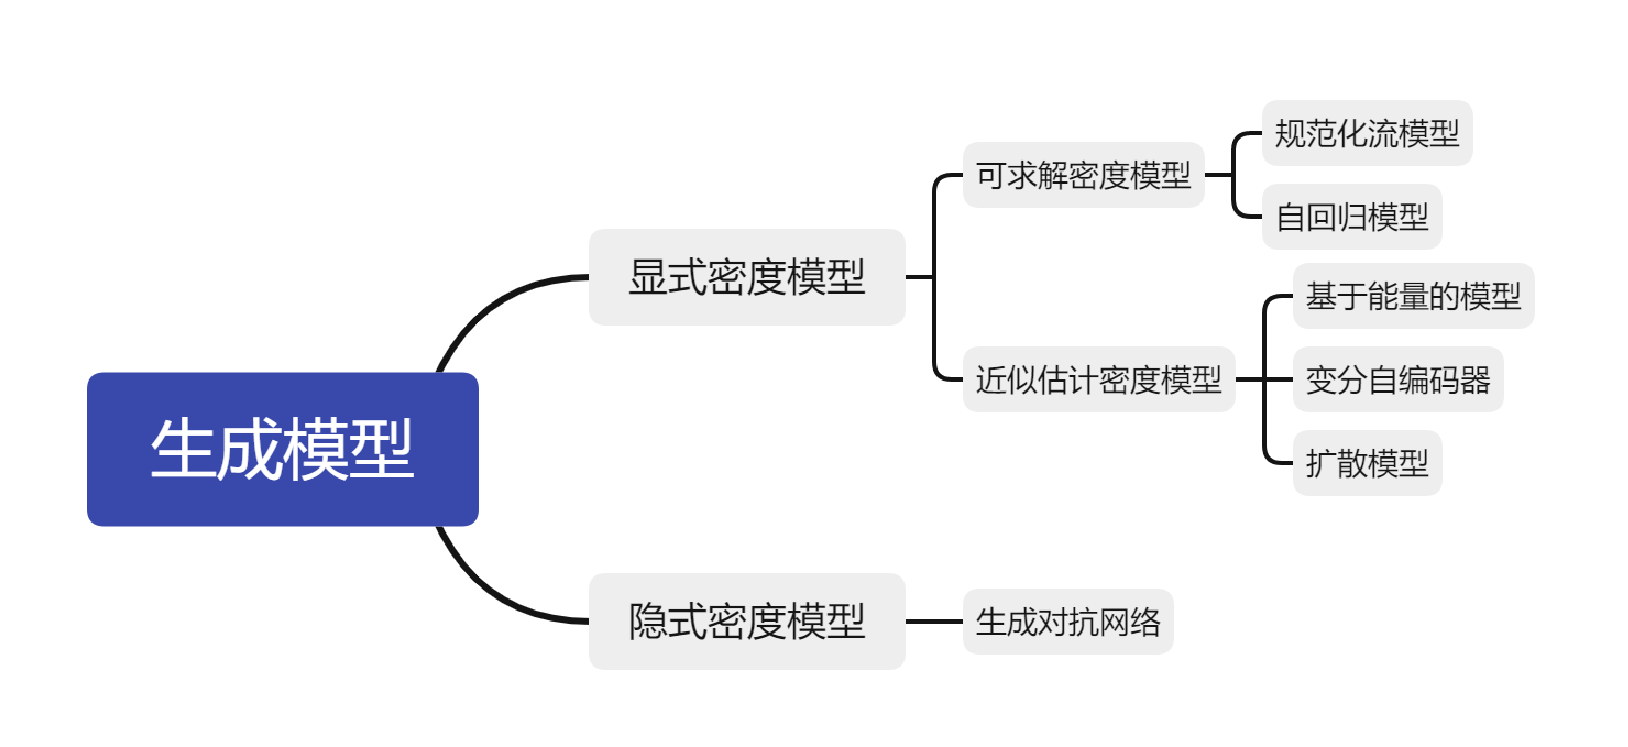
\includegraphics[width=\textwidth]{figures/gennerative_models}
    \caption{生成模型分类}\label{fig:gennerative_models}
\end{figure}



第三章使用扩散模型进行中国画生成,
根据所使用数据集与训练超参数不同,
生成不同类型的中国画。

最后对各生成模型算法与中国画生成进行总结与展望。

此外,为保持文中推理证明的完整性,在附录中添加证明所用基础知识。

% 第二章首先介绍生成模型算法基本理论,
% 第三章在变分自编码器模型基础上进行中国画生成,
% 第四章在自回归模型基础上进行中国画生成,
% 第五章在基于能量的模型基础上进行中国画生成,
% 第六章在规范化流模型基础上进行中国画生成,
% 第七章在生成对抗网络模型基础上进行中国画生成,
% 第八章在降噪扩散模型基础上进行中国画生成,
% 第九章对生成模型算法以及其在中国画上应用进行总结与展望。
\chapter{基本理论与方法}




\section{生成模型介绍}
生成模型可以通过在数据集上训练,学习数据集中样本的概率分布{$p_{data}$},
用生成模型所获得的{$p_{model}$}来近似{$p_{data}$},
训练完成获得{$p_{model}$}之后,可以通过从{$p_{model}$}中采样来生成与数据集中相似的样本。

生成模型不仅仅可以应用在近些年有较大突破的图片生成与聊天机器人,还包括很多更广泛的应用{ {\cite{goodfellow2016nips}}},如:

\begin{itemize}
    \item 生成模型的训练和采样,有助于表示和运用高维度概率分布。高维度概率分布在数学和工程领域应用广泛。
    \item 生成模型可以与强化学习相结合,如进行未来决策或对环境的模拟。
    \item 生成模型可以辅助半监督学习,如对无标签数据进行标注。
    \item 生成模型可以应用于多模态领域,如对同一输入,不仅仅生成文字,同时也可以生成图像。
    \item 从本质上来说,很多任务都需要从一些概率分布中进行采样,如提高图像分辨率,艺术创作,图像与图像之间的转换等。
\end{itemize}

很多生成模型应用极大似然估计的原理。
极大似然估计的基本思想是,
定义一个由参数{$\bm{\theta}$}确定的对概率分布的估计{$p_{model}(\bm{x};\bm{\theta})$},
之后,对训练集定义似然函数

\begin{equation}
    \label{eq:likelihood_for_training_data}
    \prod_{i=1}^{m}{p_{model}({\bm{x}}^{(i)};\bm{\theta})}
\end{equation}


式{\ref{eq:likelihood_for_training_data}}中,
{$m$}为该训练集样本数,
{$\bm{x}^{(i)}$}为训练集中样本。
\begin{align}
    \bm{\theta}^{*}
        & = \argmax_{\bm{\theta}}{\prod_{i=1}^{m}{p_{model}({\bm{x}}^{(i)};\bm{\theta})}} \label{eq:theta_star_max_1} \\
        & = \argmax_{\bm{\theta}}{\log{\prod_{i=1}^{m}{p_{model}({\bm{x}}^{(i)};\bm{\theta})}}} \label{eq:theta_star_max_2} \\
        & = \argmax_{\bm{\theta}}{{\sum_{i=1}^{m}{\log p_{model}({\bm{x}}^{(i)};\bm{\theta})}}} \label{eq:theta_star_max_3}  
\end{align}


选取参数{$\bm{\theta}^*$}使似然函数式{\ref{eq:likelihood_for_training_data}},取得最大值,
为方便计算,相比于将原似然函数进行最大化,可以将其转化之对数空间,这样可以将求积变为求和。
在式{\ref{eq:theta_star_max_2}}中,应用了对数函数为单调递增函数,不改变参数最大值取值的性质。
获得的生成模型即为{$p_{model}(\bm{x};\bm{\theta})$}。
图{\ref{fig:max_likelihood}}展示了一维极大似然估计过程,
极大似然估计从训练集中采样,
增大样本所在位置概率的同时保证概率密度总积分为1。

\begin{figure}[ht]
    \centering
    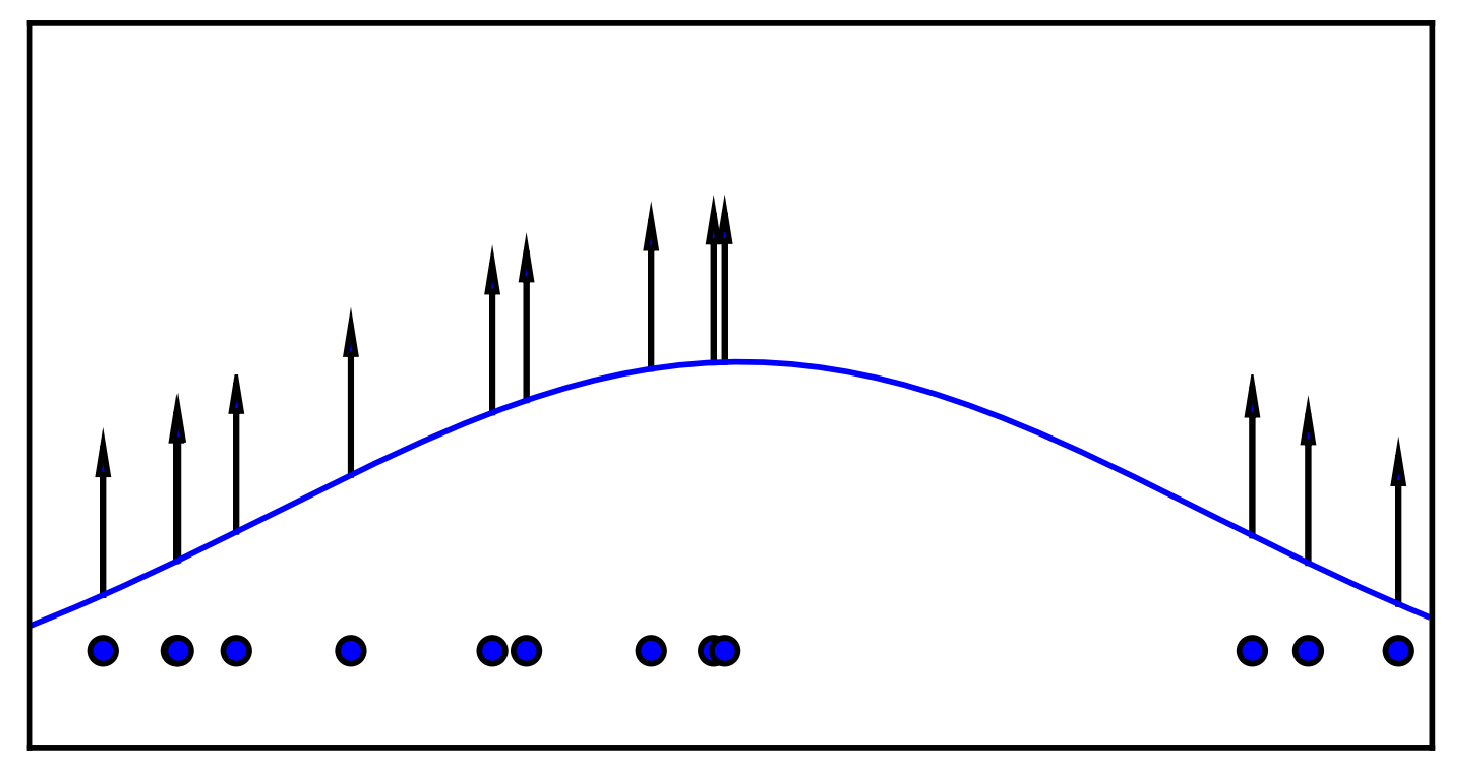
\includegraphics[width=0.8\textwidth]{figures/max_likelihood}
    \caption{一维极大似然估计过程}\label{fig:max_likelihood}
\end{figure}

从另一方面来说,
对参数{$\bm{\theta}^*$}进行极大似然估计与最小化生成模型与样本数据的实际概率分布的KL散度等价,
即:
\begin{equation}
    \label{eq:kl_divergence_max_theta}
    \bm{\theta}^{*}=\argmax_{\bm{\theta}}{D_{KL}{(p_{data}(\bm{x})||p_{model}(\bm{x};\bm{\theta}))}}
\end{equation}

可以根据如何表示或近似似然函数对生成模型进行分类。
具体地说,主要可以分为以下三类:
\begin{itemize}
    \item 可求解的显示密度模型,直接定义概率密度函数{$p_{model}(\bm{x};\bm{\theta})$},且要求其似然函数可直接求解。如规范化流模型和自回归模型。
    \item 近似估计的显示密度模型,直接定义概率密度函数{$p_{model}(\bm{x};\bm{\theta})$},且要求其似然函数可求得近似解。如基于能量的模型、变分自编码器和扩散模型。
    \item 隐式密度模型,不定义概率密度函数,而通过其他间接方式对概率分布{$p_{data}$}进行学习。如生成对抗网络。
\end{itemize}


\section{显式密度模型}\label{section:explicit_density_model}
显式密度模型直接定义概率密度函数{$p_{model}(\bm{x};\bm{\theta})$},之后即可以根据极大似然估计进行模型拟合。
显式密度模型存在的主要问题是:很难设计既可以表示样本分布又容易求解的模型。
有两种方法可以解决这个问题:
\begin{enumerate}
    \item 设计易求解的模型结构,在此基础上提高模型表达能力,即可求解密度模型。
    \item 设计模型后,通过近似方法求解似然函数,即近似估计密度模型。
\end{enumerate}


\subsection{可求解密度模型}
\subsubsection{规范化流模型}

规范化流模型通过一系列可逆变换方程,
将简单的概率分布逐渐转化为复杂的概率分布,
以希望能够拟合数据样本的概率分布。

\begin{figure}[ht]
    \centering
    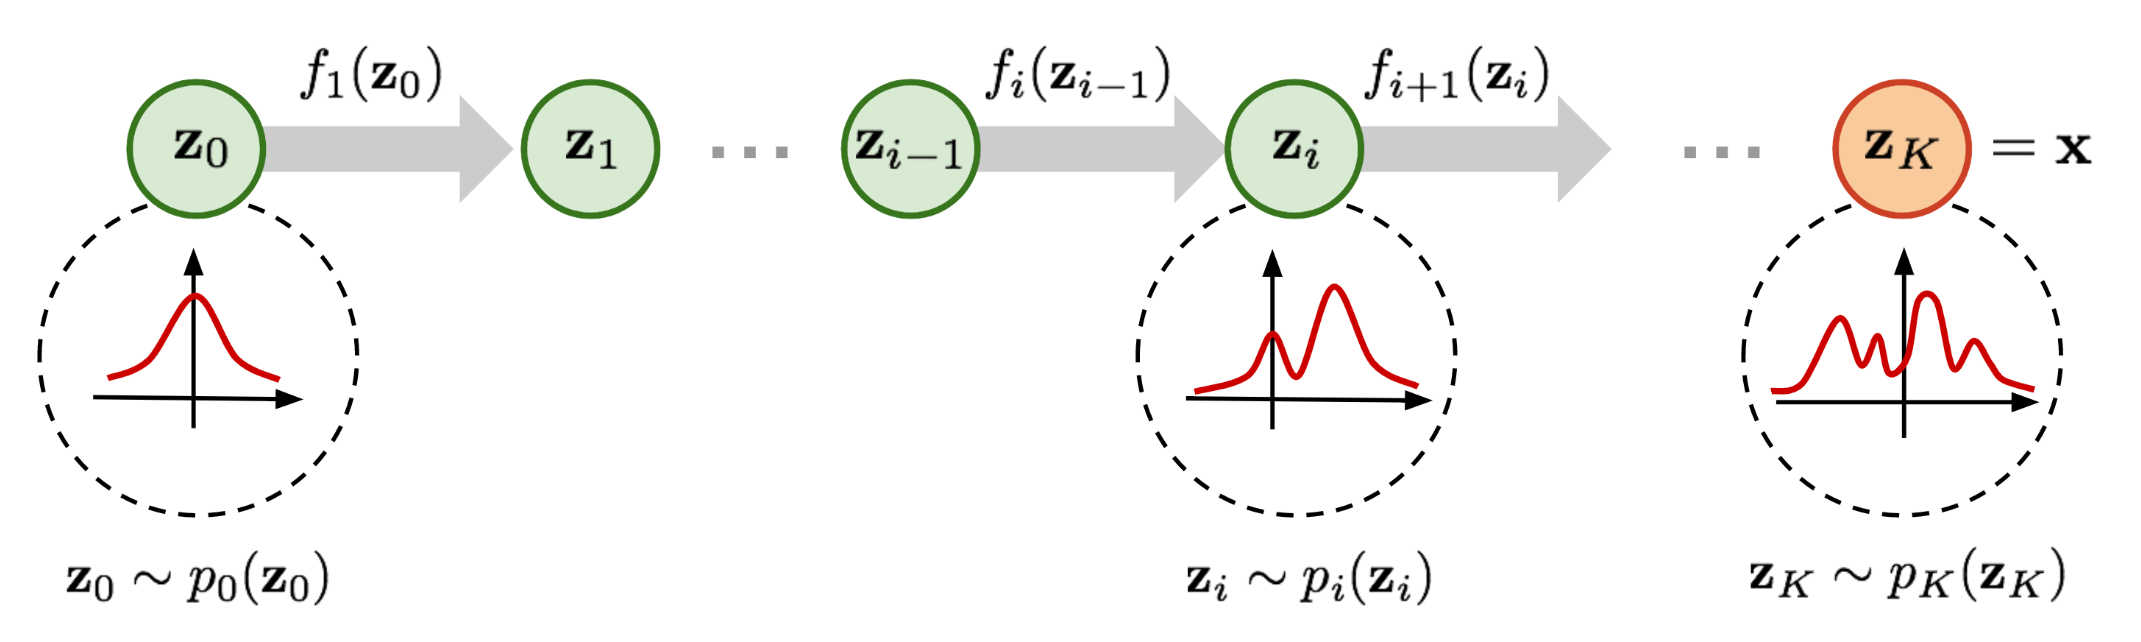
\includegraphics[width=0.8\textwidth]{figures/normalizing_flow}
    \caption{规范化流模型示意图}\label{fig:normalizing_flow}
\end{figure}
如图{\ref{fig:normalizing_flow}}所示,
\begin{align}
    \bm{z}_{i-1} &\thicksim p_{i-1}(\bm{z}_{i-1}) \\
    \bm{z}_i&=f_i(\bm{z}_{i-1})
\end{align}
由反函数定理,
\begin{equation}
    \bm{z}_{i-1}=f_{i}^{-1}(\bm{z}_i)
\end{equation}
由附录式{\ref{eq:mutivariable_change_variable_in_probability}},
\begin{equation}
    \label{eq:normalizing_flow_p_of_z}
    p_i(\bm{z}_i)=p_{i-1}(f_i^{-1}(\bm{z}_i))\left\rvert \det \frac{df_i^{-1}}{d\bm{z}_i}\right\rvert
\end{equation}
为获得{$p_i(\bm{z}_i)$}与{$p_{i-1}(\bm{z}_{i-1})$}之间的关系,
对式{\ref{eq:normalizing_flow_p_of_z}}进行变形:
\begin{align}
    p_i(\bm{z}_i)
    & = p_{i-1}(f_i^{-1}(\bm{z}_i))\left\rvert \det\frac{df_{i}^{-1}}{d\bm{z}_i} \right\rvert \\
    & = p_{i-1}(\bm{z}_{i-1})\left\rvert \det {(\frac{df_{i}}{d\bm{z}_{i-1}})}^{-1} \right\rvert &\mbox{(根据式{\ref{eq:inverse_function_theorem_application}})}\\
    & = p_{i-1}(\bm{z}_{i-1})\left\rvert \det \frac{df_{i}}{d\bm{z}_{i-1}} \right\rvert^{-1}  &\mbox{(根据式{\ref{eq:determinant_of_inverse_matrix}})} \label{eq:normalizing_flow_change_variable}
\end{align}
对式{\ref{eq:normalizing_flow_change_variable}}进行对数化得:
\begin{equation}
    \label{eq:normalizing_flow_flow_equation}
    \log p_i(\bm{z}_i)=\log p_{i-1}(\bm{z}_{i-1})-\log \left\rvert \det \frac{df_{i}}{d\bm{z}_{i-1}}   \right\rvert
\end{equation}
连续应用式{\ref{eq:normalizing_flow_flow_equation}},
对{$\bm{x}$}不断变换可得其关于简单概率分布变量{$\bm{z}$}的表达式,即:
\begin{align}
    \bm{x}=\bm{z}_K 
    & =f_K\circ f_{K-1} \circ \cdots  \circ f_1(\bm{z}_0) \\
    \log p(\bm{x})= \log p_K(\bm{z}_K)
    & =\log p_{K-1}(\bm{z}_{K-1}) - \log \left| \det \frac{df_K}{d\bm{z}_{K-1}} \right| \\
    & =\log p_{K-2}(\bm{z}_{K-2}) - \log \left| \det \frac{df_{K-1}}{d\bm{z}_{K-2}} \right| - \log \left| \det \frac{df_K}{d\bm{z}_{K-1}} \right| \\
    & = \cdots \\
    & = \log p_0(\bm{z}_0) - \sum_{i=1}^{K} \log \left| \det \frac{df_i}{d\bm{z}_{i-1}}\right|
\end{align}

所谓规范化流模型中的流指的是一系列随机变量之间的代换,
即不断应用{$\bm{z}=f_i(\bm{z}_{i-1})$}。
规范化流是指由一系列分布{$p_i$}组成的完整链式过程{ {\cite{weng2018flow}}}。

由上述计算过程,转换函数{$f_i$}需要满足两个条件:
\begin{itemize}
    \item 具备可逆性质;
    \item 雅可比矩阵容易计算。
\end{itemize}

\subsubsection{自回归模型}

自回归模型将生成问题简化成顺序问题,即通过之前的顺序值来预测下一个值。
一般来说,自回归模型对于高维数据{$x$}将其联合概率分布化为条件概率的乘积的形式:
\begin{equation}
    \label{eq:autoregressive_model_defination}
    p(\bm{x})=p(x_1,\ldots ,x_n)=\prod_{i=1}^{n}p(x_i|x_1,\ldots ,x_{i-1})
\end{equation}
对条件概率的模拟比直接对联合概率分布进行建模更加容易。

具体而言,为便于求解可以假定每一个变量只依赖于不超过一定数量的变量,比如两个变量,即:
\begin{equation}
    p(\bm{x})=p(x_1)p(x_2|x_1)\prod_{d=3}^{D}p(x_d \vert x_{d-1},x_{d-2})
\end{equation}

\begin{figure}[ht]
    \centering
    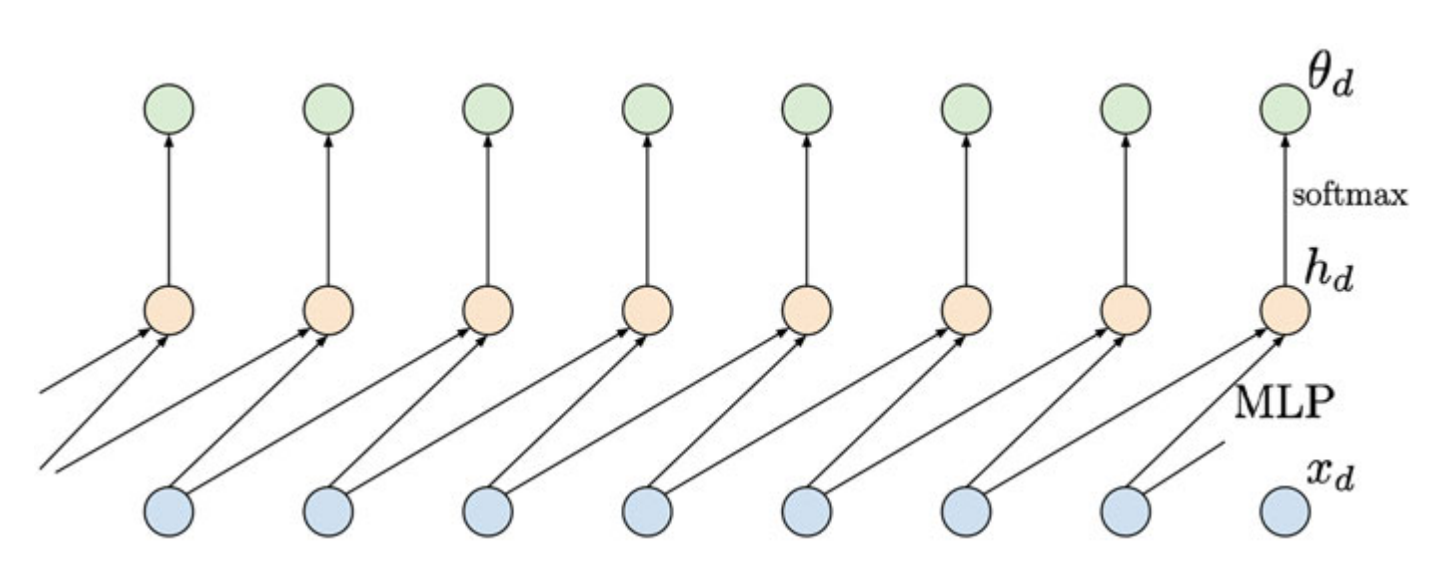
\includegraphics[width=0.8\textwidth]{figures/autoregressive_model_finite_memory}
    \caption{自回归模型依赖两变量示意图}\label{fig:autoregressive_model_finite_memory}
\end{figure}
可以使用多层感知机预测{$x_d$}的概率分布,
图{\ref{fig:autoregressive_model_finite_memory}}表示使用多层感知机进行预测{$x_d$}的概率分布。
最下面的蓝色结点表示输入,
中间层橘色结点表示多层感知机对前两个数据处理后的输出,
最后绿色点表示通过归一化指数函数输出的概率{$p(x_d \rvert x_{d-1},x_{d-2})$},即{$\theta_d$}。
但是,这种假设,即每一个变量只依赖于不超过一定数量的变量,对模型造成了很大的限制。
通过循环神经网络可以对以往信息进行更长期的保存{ {\cite{Jakub2022deep}}},即:
\begin{equation}
    \label{eq:autoregressive_model_rnn}
    p(x_d \rvert \bm{x}_{<d})=p(x_d \vert RNN(x_{d-1},h_{d-1}))
\end{equation}

式{\ref{eq:autoregressive_model_rnn}}中,
{$h_d=RNN(x_d, h_{d-1})$},{$h_d$}可以看作对所有历史信息的保存,可称为隐环境。
图{\ref{fig:autoregressive_model_rnn}}表示使用循环神经网络RNN预测{$x_d$}的概率分布。
最下面的蓝色结点表示输入,
中间层橘色结点表示循环神经网络对前两个输入数据与隐环境处理后的输出,
最后绿色结点表示通过归一化指数函数后输出的概率{$p(x_d \rvert x_{d-1},x_{d-2})$},即{$\theta_d$}。
\begin{figure}[ht]
    \centering
    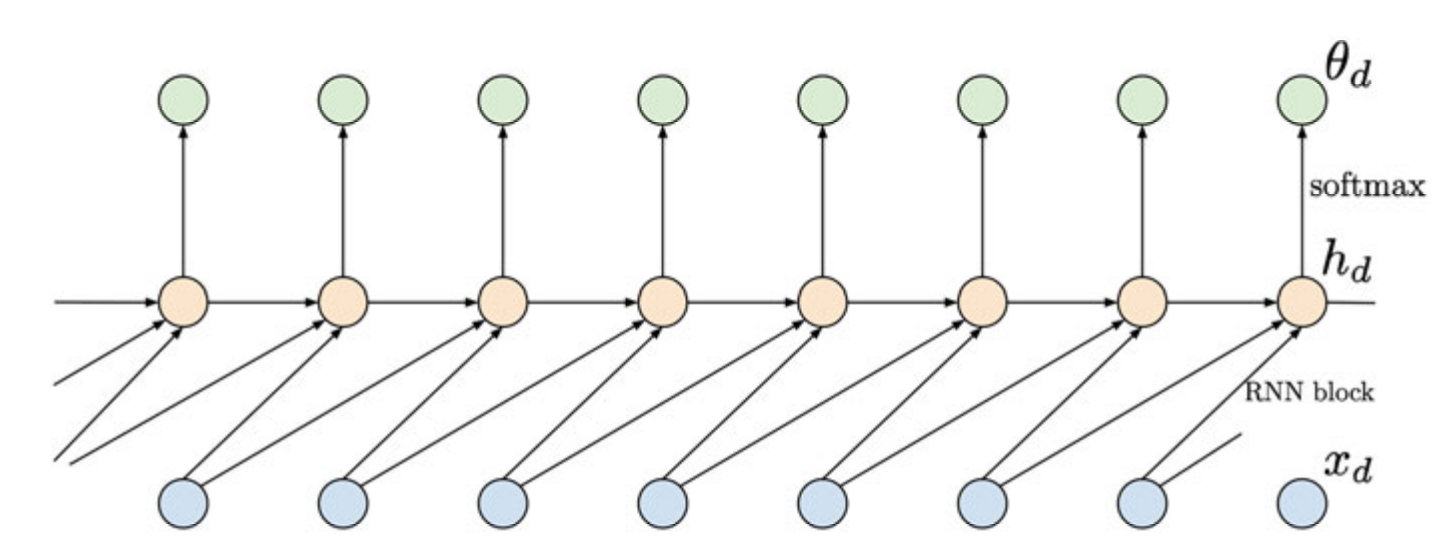
\includegraphics[width=0.8\textwidth]{figures/autoregressive_model_rnn}
    \caption{循环神经网络示意图}\label{fig:autoregressive_model_rnn}
\end{figure}

此外,transformer也属于自回归模型,transformer通过自注意力机制来对历史信息进行处理。


\subsection{近似估计密度模型}
\subsubsection{基于能量的模型}
%玻尔兹曼机
%Contrastive Divergence
%Langevin Dynamics
基于能量的模型的诞生受到对物理系统建模的启发——
一个事件的概率可以由玻尔兹曼分布式{\ref{eq:boltzmann_equation}}表示{\cite{lippe2022uvadlc}}。
如果一个神经网络{$E_{\theta}(\bm{x})$}只有一个输出神经元,
{$\theta$}表示神经网络的参数,
{$\bm{x}$}表示神经网络的输入,
其输出结果为实值标量,
那么有:
\begin{equation}
    \label{eq:energy_based_model_probability}
    q_{\theta}(\bm{x})=\frac{\exp(-E_{\theta}(\bm{x}))}{Z_{\theta}}
    \mbox{ ,其中}
    Z_{\theta}=
    \begin{cases}
        \int_{\bm{x}} \exp(-E_{\theta}(\bm{x})) \,d\bm{x}  & \bm{x}\mbox{为连续变量}\\
        \sum_{\bm{x}}\exp(-E_{\theta}(\bm{x}))       & \bm{x}\mbox{为离散变量}
    \end{cases}
\end{equation}

式{\ref{eq:energy_based_model_probability}}中,
指数函数保证所得概率大于0,
在{$E_{\theta}(\bm{x})$}前添加负号以表示{$E_{\theta}$}为能量函数:
样本点概率取值越高则其能量越低,
概率取值越低则具有更高的能量。
{$Z_{\theta}$}是归一化项用来保证概率密度积分或和为1,
如式{\ref{eq:energy_based_model_integrates_sum_to_1}}所示:
\begin{equation}
    \label{eq:energy_based_model_integrates_sum_to_1}
    \int_{\bm{x}} q_{\theta}(\bm{x}) \,d\bm{x} 
    = \int_{\bm{x}} \frac{\exp(-E_{\theta}(\bm{x}))}{\int_{\bm{\hat{x}}} \exp(-E_{\theta}(\bm{\hat{x}})) \,d\bm{\hat{x}}} \,d\bm{x}
    =\frac{\int_{\bm{x}} \exp(-E_{\theta}(\bm{x})) \,d\bm{x}}{\int_{\bm{\hat{x}}} \exp(-E_{\theta}(\bm{\hat{x}})) \,d\bm{\hat{x}}}
    =1
\end{equation}

式{\ref{eq:energy_based_model_probability}}与式{\ref{eq:energy_based_model_integrates_sum_to_1}}中,
{$q_{\theta}(\bm{x})$}为{$p(\bm{x})$}的近似,通过训练,可以使{$q_{\theta}(\bm{x})$}逐渐接近{$p(\bm{x})$}。

对于基于能量的模型,
{$E_{\theta}$}可以根据需要灵活选择。
由于归一化常数{$Z_{\theta}$}未知,
无法直接计算对数似然函数,
且由于{$Z_{\theta}$}不一定能保证不变,
不可直接对未进行归一化的概率{$\exp(-E_{\theta}(\bm{x}_{train}))$}极大化,
即不一定保证训练样本点相比其他数据点有更高的概率出现。
对于极大似然函数的计算,可以通过对比散度方法来进行近似。
通过比较不同数据点的似然来进行计算,
根据附录式{$\ref{eq:contrastive_divergence_partial_negative_log_likelihood}$}可得负对数似然函数,
\begin{align}
    \nabla _{\theta} Loss(q_{\theta}(\bm{x}))
    &= - \mathbb{E}_{p(\bm{x})}\left[ \nabla_{\theta} \log q_{\theta}(\bm{x}) \right] \label{eq:energy_based_model_nnl_origin} \\
    &= \mathbb{E}_{p(\bm{x})}\left[ \nabla_{\theta} E_{\theta}(\bm{x}) \right] - \mathbb{E}_{q_{\theta}(\bm{x})}\left[ \nabla_{\theta} E_{\theta}(\bm{x}) \right]  \label{eq:energy_based_model_nnl_contrastive_divergence}
\end{align}

式{\ref{eq:energy_based_model_nnl_origin}}即为需要最小化的损失函数。
对于式{\ref{eq:energy_based_model_nnl_contrastive_divergence}},
从直观上理解,
第一项表示最小化数据集中样本点的能量,以增加其概率;
第二项表示最大化随机生成的样本点的能量,以减小其概率。
图{\ref{fig:energy_based_model_contrastive_divergence_training}}中,
{$f_{\theta}$}表示{$\exp (-E_{\theta}(\bm{x}))$},
通过训练,可以降低数据集中样本的能量函数值,增大随机生成样本的能量函数值。
\begin{figure}[ht]
    \centering
    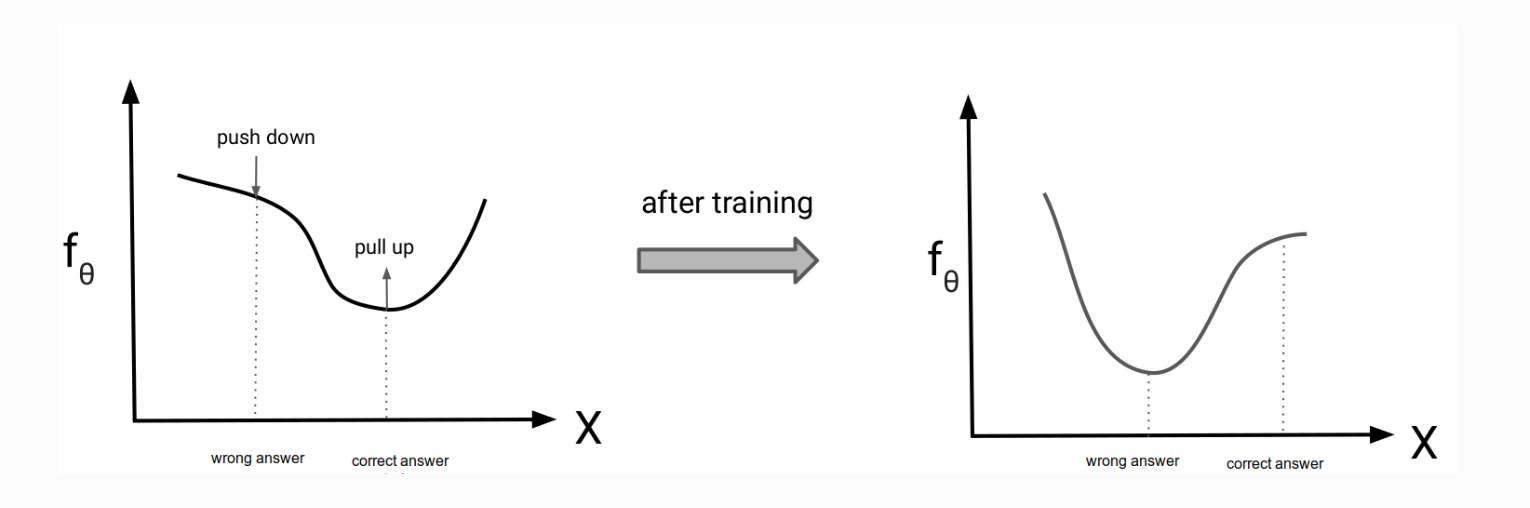
\includegraphics[width=1\textwidth]{figures/energy_based_model_contrastive_divergence_training}
    \caption{对比散度训练前后对比}\label{fig:energy_based_model_contrastive_divergence_training}
\end{figure}

式{\ref{eq:energy_based_model_nnl_contrastive_divergence}}中,
需要对概率分布{$q_{\theta}(\bm{x})$}采样。
可以应用朗志万动力学与马尔科夫链蒙特卡洛结合的方法采样,
即从随机数据点开始,
根据能量函数的梯度{$\nabla_{\bm{x}}E_{\theta}(\bm{x})$},使数据点的值向能量函数降低的方向移动。
此外,为避免陷入局部最小值,
需要在每一次更新梯度时添加噪声{$\omega \backsim \mathcal{N}(0,\sigma) $}。
理论上讲,根据梯度进行足够多次数据点取值更新,即可以准确地从概率分布{$q_{\theta}(\bm{x})$}采样,
但在实际中,通常将马尔科夫链的链长限制为{$K$},即进行{$K$}次取值更新。
算法{\ref{alg:energy_based_model_sampling}}为从基于能量的模型采样的算法。
\begin{algorithm}[ht]
    \caption{从基于能量的模型采样}\label{alg:energy_based_model_sampling}
    \begin{algorithmic}[1]
    \STATE{从高斯分布或均匀分布中采样{$\bm{\tilde{x}}^{0}$}}
    \FOR{采样步骤 {$k=1$}到 {$K$} }
    \STATE{{$\bm{\tilde{x}}^{k} \leftarrow \bm{\tilde{x}}^{k-1}- \eta\nabla_{\bm{x}}E_{\theta}(\bm{\tilde{x}}^{k-1}) + \omega  $},其中{$\omega \sim \mathcal{N}(0,\sigma)$}}
    \ENDFOR
    \STATE{$\bm{x}_{sample} \leftarrow \bm{\tilde{x}}^{K}$}
    \end{algorithmic}
\end{algorithm}



\subsubsection{变分自编码器}

自编码器是一个包含了两部分的神经网络,
其编码器可以将原始高维输入映射到低维隐变量空间,
解码器可以将隐变量空间中的低维表示恢复成原始输入{\cite{weng2018VAE}}。
通过使用自编码器,可以对数据进行更高效地压缩。
\begin{figure}[ht]
    \centering
    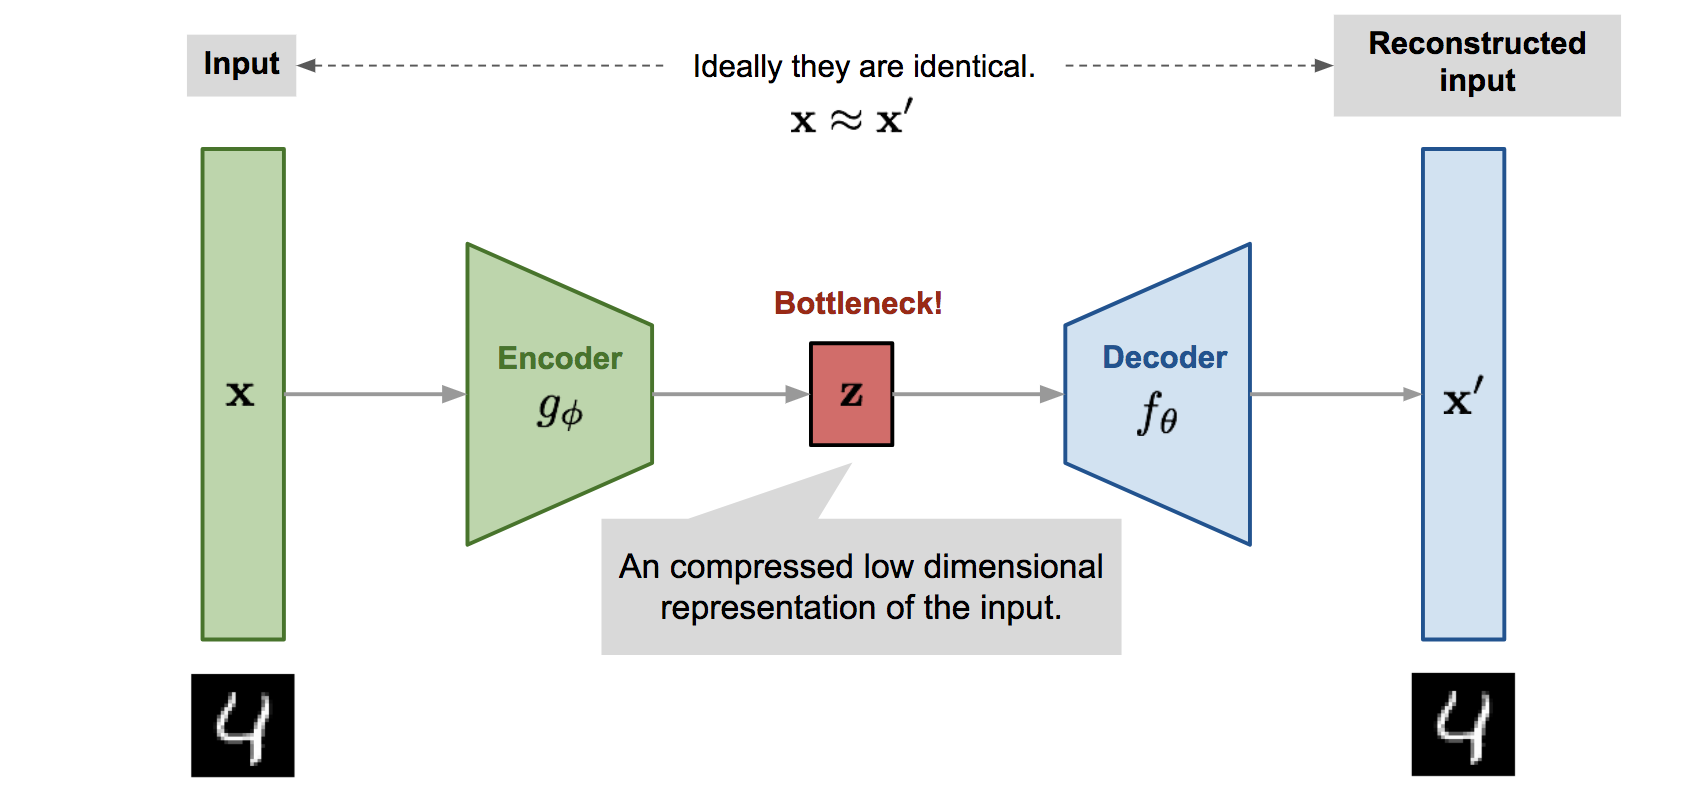
\includegraphics[width=1\textwidth]{figures/autoencoder}
    \caption{自编码器示意图}\label{fig:autoencoder}
\end{figure}

图{\ref{fig:autoencoder}}中,
{$\bm{x}$}表示样本,
{$\bm{x}^{'}$}表示对原始样本的重构,
{$\bm{z}$}表示样本在隐变量空间的表示,
{$g_{\phi}(.)$}表示由参数{$\phi$}确定的编码器函数,
{$f_{\theta}(.)$}表示由参数{$\theta$}确定的解码器函数。
\begin{equation}
    \label{eq:vae_encoder}
    \bm{z}=g_{\phi}(\bm{x})
\end{equation}
\begin{equation}
    \label{eq:vae_decoder}
    \bm{x}^{'}=f_{\theta}(g_{\phi}(\bm{x}))
\end{equation}

参数{$(\theta,\phi)$}可以通过比较原始样本值{$\bm{x}$}与重构样本值{$\bm{x}^{'}$}来学习,
如使用均方误差:
\begin{equation}
    \label{eq:autoencoder_loss}
    L_{AE}(\theta,\phi)=\frac{1}{n} \sum_{i=1}^{n}(\bm{x}^{(i)} - f_{\theta}(g_{\phi}(\bm{x})))
\end{equation}

为避免过拟合,
降噪自编码器{ {\cite{vincent2008extracting}}}对原始样本添加随机噪声:
\begin{align}
    \hat{\bm{x}}^{(i)} 
    & \backsim \mathcal{M}_{\mathcal{D}}(\hat{\bm{x}}^{(i)} \mid \bm{x}^{(i)}) \label{eq:denoising_autoencoder_corrupt}   \\
    L_{DAE}(\theta,\phi)
    &=\frac{1}{n} \sum_{i=1}^{n}(\bm{x}^{(i)} - f_{\theta}(g_{\phi}(\hat{\bm{x}}^{(i)} ))) \label{eq:denoising_autoencoder_loss}
\end{align}

式{\ref{eq:denoising_autoencoder_corrupt}}中,
{$\hat{\bm{x}}^{(i)} $}表示对原始样本值{$\bm{x}$}添加随机噪声或者进行掩码处理后的值,
{$\mathcal{D}$}为原始样本所在数据集,
{$ \mathcal{M}_{\mathcal{D}}$}表示从原始样本到{$\hat{\bm{x}}^{(i)} $}的映射。
式{\ref{eq:denoising_autoencoder_loss}}与式{\ref{eq:autoencoder_loss}}相比,
不再将重构样本与原始样本{$\bm{x}$}进行比较,
而是与添加随机噪声或进行掩码处理后的{$\hat{\bm{x}}^{(i)} $}进行比较。
图{\ref{fig:denoising_autoencoder_architecture}}为降噪自编码器结构图。
\begin{figure}[ht]
    \centering
    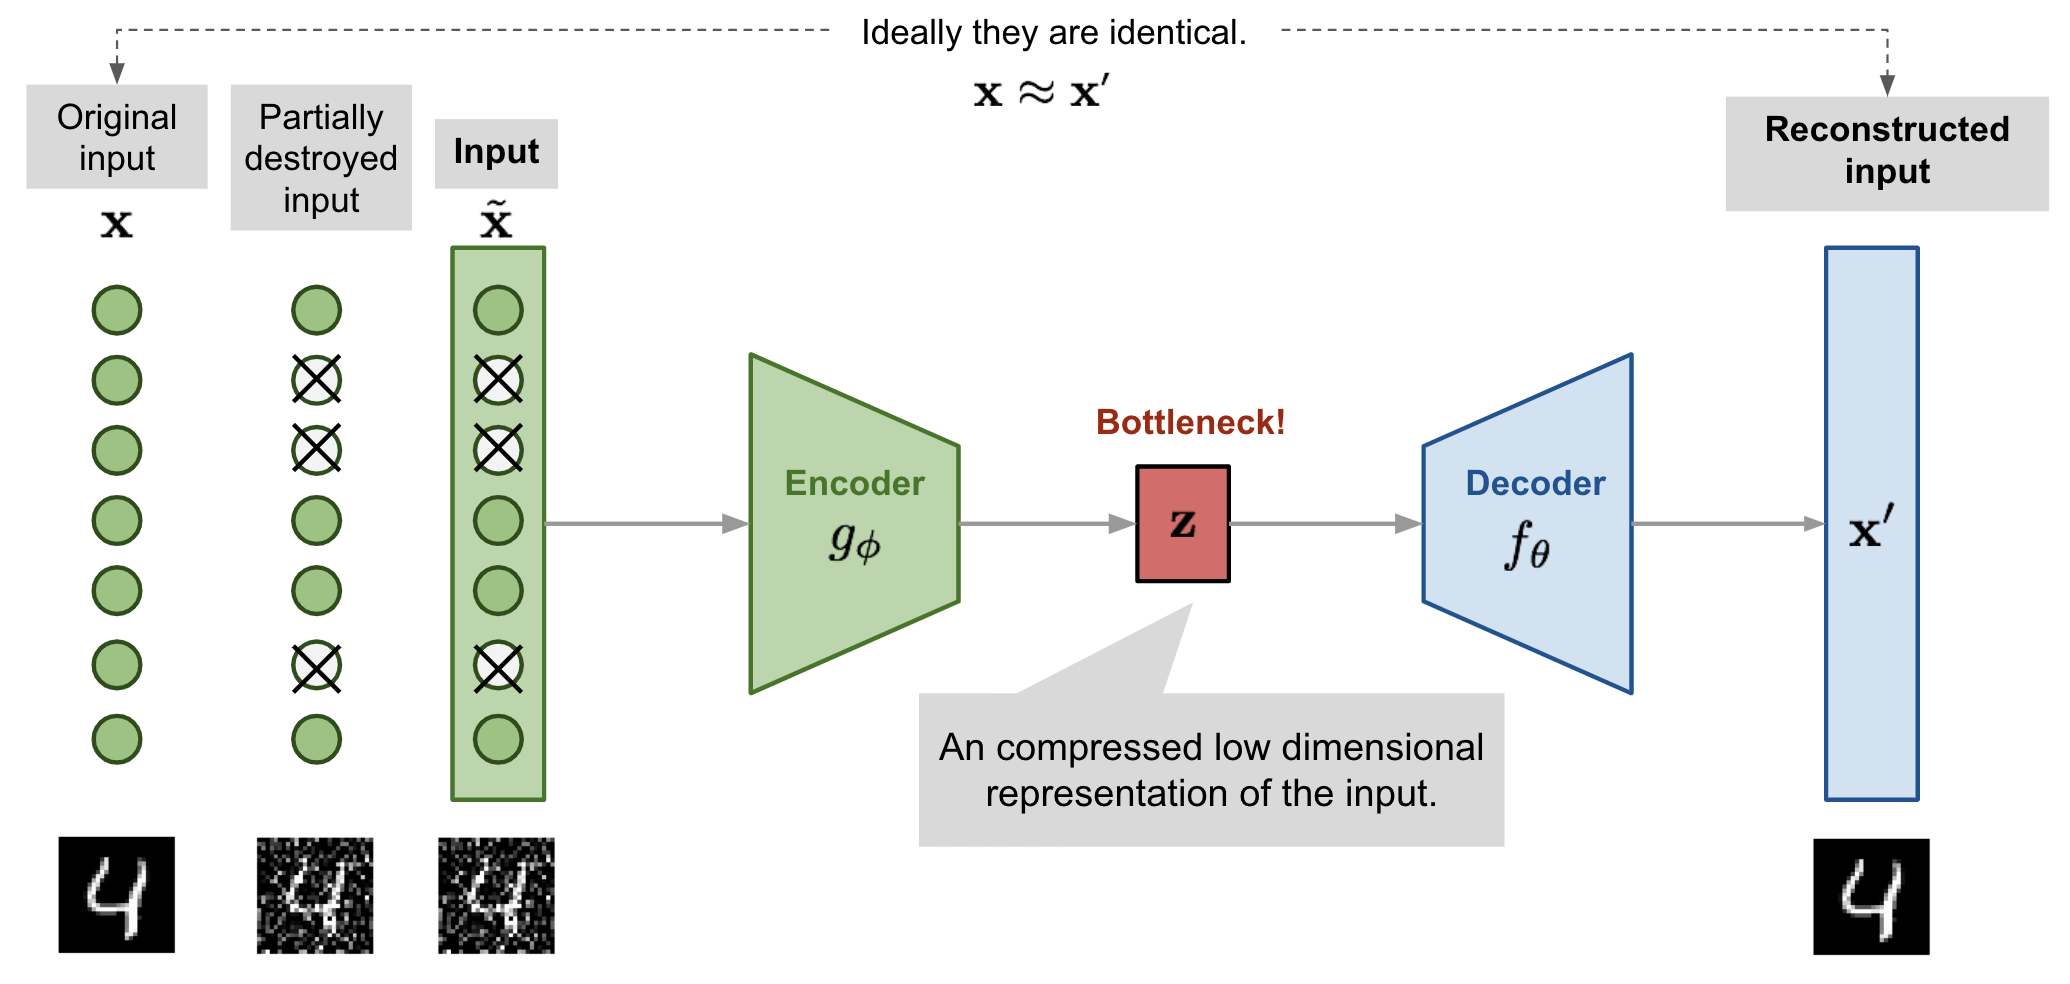
\includegraphics[width=1\textwidth]{figures/denoising_autoencoder_architecture}
    \caption{降噪自编码器结构}\label{fig:denoising_autoencoder_architecture}
\end{figure}

相比于自编码器和降噪自编码器,
变分自编码器并不将样本映射到一个固定的向量
而是映射到一个由参数{$\theta$}确定的概率分布{$p_{\theta}$}。
输入样本{$\bm{x}$}和隐变量{$\bm{z}$}的关系可以定义为:
\begin{itemize}
    \item 先验概率{$p_{\theta}(\bm{z})$};
    \item 似然函数{$p_{\theta}(\bm{x}\mid \bm{z})$};
    \item 后验概率{$p_{\theta}(\bm{z}\mid \bm{x})$}。
\end{itemize}

若知道概率分布{$p_{\theta}$}的真实参数值{$\theta ^{*}$},
则生成样本点某一维度的值{$\bm{x}^{(i)}$}(如图片样本的一个像素值)需要两个步骤:
\begin{enumerate}
    \item 从先验分布{$p_{\theta^{*}}(\bm{z})$}中采样获得{$\bm{z}^{(i)}$};
    \item 从条件概率{$p_{\theta^{*}}(\bm{x}\mid \bm{z}=\bm{z}^{(i)})$}中生成值{$\bm{x}^{(i)}$}。
\end{enumerate}

最优参数值{$\theta^{*}$}可以通过最大化生成真实数据样本的概率获得,即:
\begin{equation}
    \label{eq:vae_maximum_likelihood}
    \theta ^{*}=\argmax_{\theta}\prod_{i=1}^{n}p_{\theta}(\bm{x}^{(i)})
\end{equation}
取对数可得:
\begin{equation}
    \label{eq:vae_maximux_log_likelihood}
    \theta ^{*}=\argmax_{\theta}\sum_{i=1}^{n}\log p_{\theta}(\bm{x}^{(i)})
\end{equation}
式{\ref{eq:vae_maximux_log_likelihood}}中,
{$p_{\theta}(\bm{x}^{(i)})$}
可以表示为:
\begin{equation}
    \label{eq:var_probability_of_xi}
    p_{\theta}(\bm{x}^{(i)})=\int p_{\theta}(\bm{x}^{(i)} \mid \bm{z}) p_{\theta}(\bm{z}) d\,{\bm{z}}
\end{equation}

但由于某些隐变量无法积分或计算开销巨大,
式{\ref{eq:var_probability_of_xi}}无法直接计算。
可用证据下界式{\ref{eq:evidence_lower_bound}}来近似对数似然函数。
使用证据下界可以获得对后验概率{$p_{\theta}(\bm{z}\mid\bm{x})$}的近似,
即由参数{$\phi$}确定的{$q_{\phi}(\bm{z}\mid\bm{x})$}。
图{\ref{fig:vae_elbo}}中,
近似函数{$q_{\phi}(\bm{z}\mid\bm{x})$}定义了编码器,
条件概率{$p_{\theta}(\bm{x}\mid\bm{z})$}定义了解码器。
\begin{figure}[ht]
    \centering
    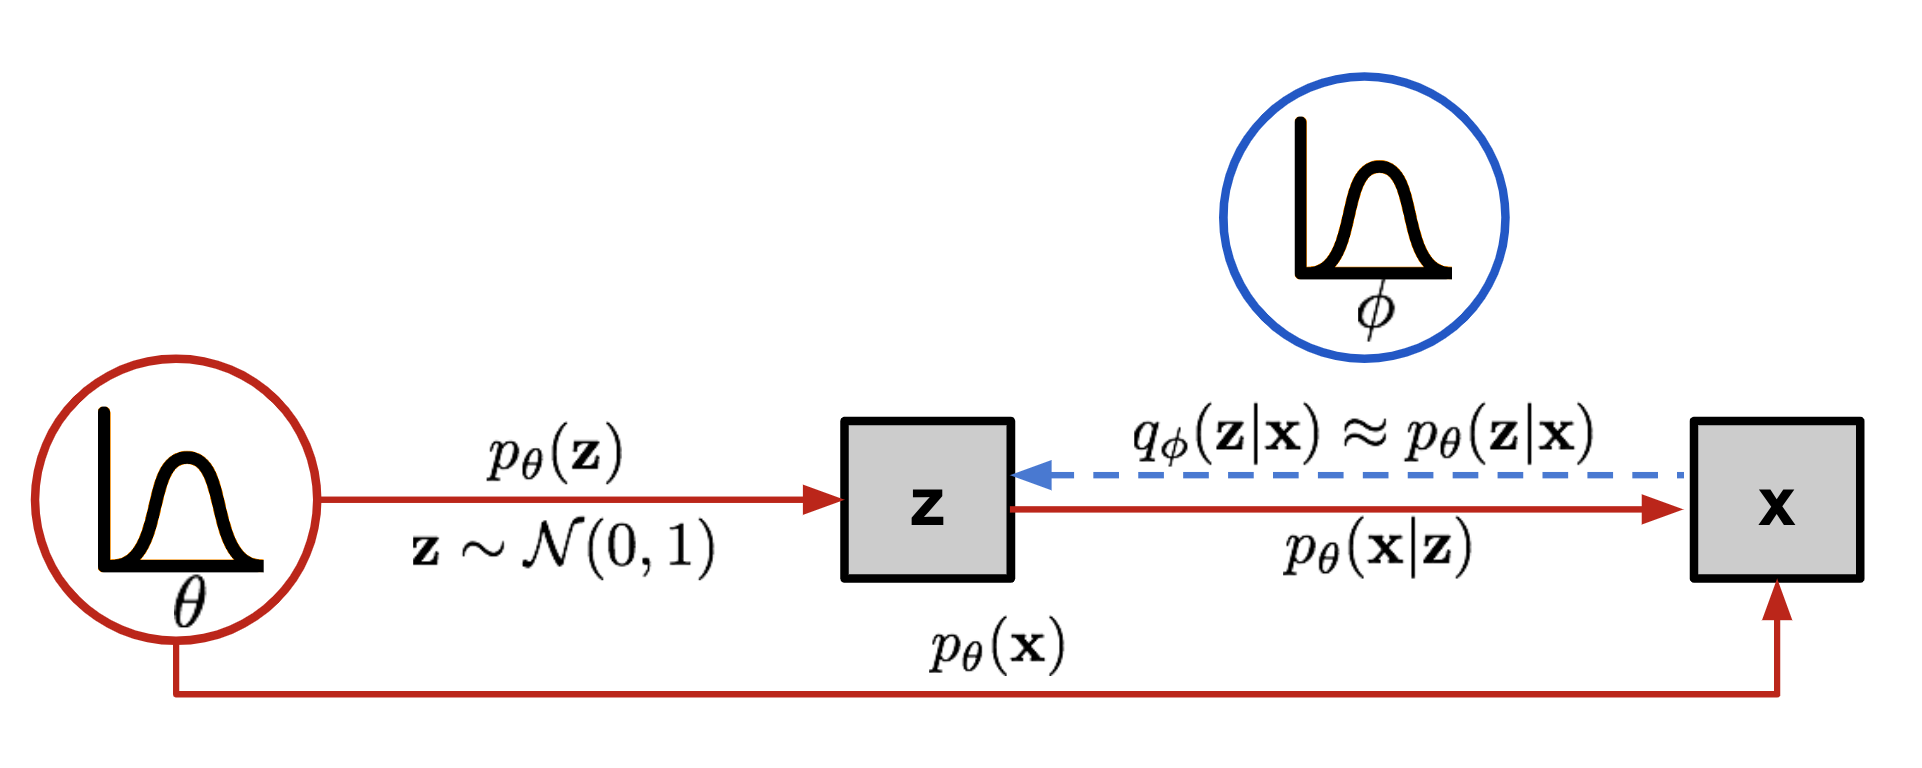
\includegraphics[width=\textwidth]{figures/vae_elbo}
    \caption{使用ELBO近似变分自编码器对数似然函数}\label{fig:vae_elbo}
\end{figure}

对证据下界式{\ref{eq:evidence_lower_bound}}变形可得:
\begin{align}
    \mathbb{E}_{q_{\phi}(\bm{z}|\bm{x})}\left[\log\frac{p(\bm{x},\bm{z})}{q_{\phi}(\bm{z}\mid\bm{x})}\right]
    &=\mathbb{E}_{q_{\phi}(\bm{z}|\bm{x})}\left[\log\frac{p_{\theta}(\bm{x}\mid \bm{z})p(\bm{z})}{q_{\phi}(\bm{z}\mid\bm{x})}\right] \\
    &=\mathbb{E}_{q_{\phi}(\bm{z}|\bm{x})}\left[\log p_{\theta}(\bm{x}\mid \bm{z})\right] + \mathbb{E}_{q_{\phi}(\bm{z}|\bm{x})}\left[\log\frac{p(\bm{z})}{q_{\phi}(\bm{z}\mid\bm{x})}\right]\\
    &=\underbrace{\mathbb{E}_{q_{\phi}(\bm{z}|\bm{x})}\left[\log p_{\theta}(\bm{x}\mid \bm{z})\right] }_{\mbox{重构项}} -\underbrace{ D_{KL}(q_{\phi}(\bm{z}\mid \bm{x}) \mid \mid p(\bm{z}))}_{\mbox{先验匹配项}}  \label{eq:vae_elbo_dissect}
\end{align}

式{\ref{eq:vae_elbo_dissect}}中,
重构项度量了解码器相对于变分分布{$q_{\phi}(\bm{z}\mid \bm{x})$}的重构似然函数{$p_{\theta}(\bm{x}\mid \bm{z})$},
从而使学到的分布可以对隐变量有效地建模,以便于可以通过{$p_{\theta}(\bm{x}\mid\bm{z})$}进行原样本重构。
先验匹配项度量了学到的变分分布与隐变量先验分布的相似度,
从而保证编码器能够真正学到隐变量分布而不是记忆原样本到隐变量的映射。
最大化证据下界等价于最大化重构项和最小化先验匹配项。
\begin{figure}[ht]
    \centering
    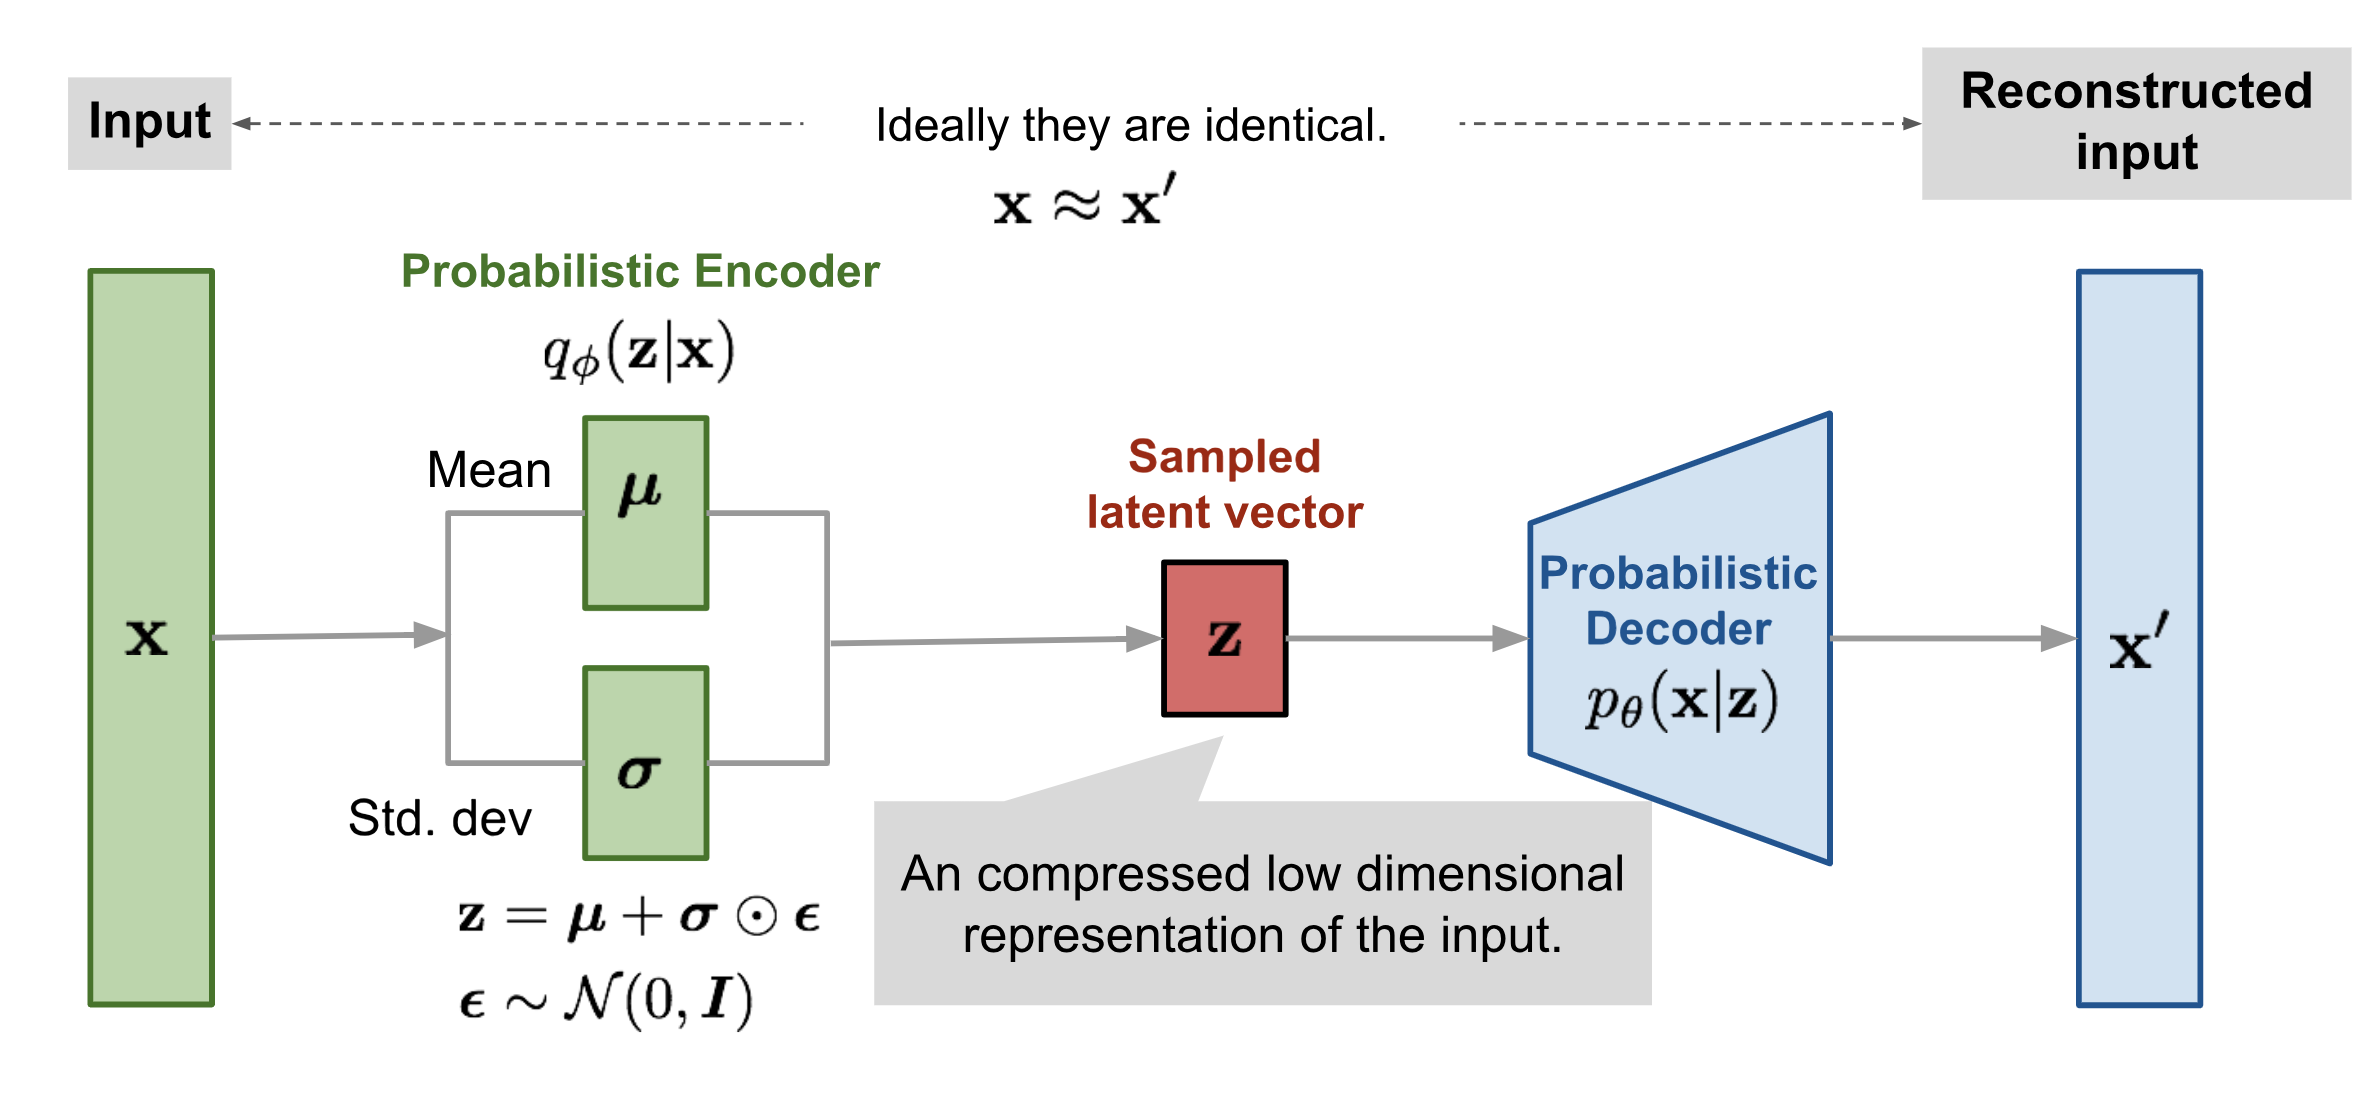
\includegraphics[height=0.4\textwidth]{figures/vae}
    \caption{变分自编码器}\label{fig:vae}
\end{figure}


变分自编码器中,通常编码器都为具有对角协方差矩阵的多变量高斯分布,隐变量的先验分布为多变量标准高斯分布:
\begin{equation}
    \label{eq:vae_q_phi_z_mid_x_gaussian}
    q_{\phi}(\bm{z}\mid\bm{x})=\mathcal{N}(\bm{z};\bm{\mu}_{\phi}(\bm{x},\bm{\sigma}_{\phi}^{2}(\bm{x})\bm{I}))
\end{equation}
\begin{equation}
    \label{eq:vae_p_z_gaussian}
    p(\bm{z})=\mathcal{N}(\bm{z};\bm{0},\bm{I})
\end{equation}

因此,
由式{\ref{eq:vae_q_phi_z_mid_x_gaussian}}和式{\ref{eq:vae_p_z_gaussian}}可以计算式{\ref{eq:vae_elbo_dissect}}中的先验匹配项。
而式{\ref{eq:vae_elbo_dissect}}中的重构项可以由蒙特卡洛方法进行估计,
即:
\begin{align}
   &\argmax_{\phi,\theta} \mathbb{E}_{q_{\phi}(\bm{z}|\bm{x})}\left[\log p_{\theta}(\bm{x}\mid \bm{z})\right]  - D_{KL}(q_{\phi}(\bm{z}\mid \bm{x}) \mid \mid p(\bm{z})) \label{eq:vae_argmax-elbo} \\
   &\approx  \argmax_{\phi,\theta} \sum_{l=1}^{L} \log p_{\theta}(\bm{x}\mid \bm{z}^{(l)}) - D_{KL}(q_{\phi}(\bm{z}\mid \bm{x}) \mid \mid p(\bm{z}))  \label{eq:vae_max_elbo_approx}
\end{align}
式{\ref{eq:vae_max_elbo_approx}}中,{${\bm{z}^{(l)}}_{l=1}^{L}$}为关于数据集中每个样本{$\bm{x}$}从{$q_{\phi}(\bm{z}\mid\bm{x})$}中获得的采样。

但由于通过随机过程获得的采样{$\bm{z}^{(l)}$}不可微,
无法计算梯度,
根据重参数方法式{\ref{eq:reparameterization_trick}}可得:
\begin{equation}
    \label{eq:vae_reparameterization_trick}
    \bm{z}=\bm{\mu}_{\phi}{(\bm{x})}+\bm{\sigma}_{\phi}(\bm{x})\odot \bm{\epsilon} \mbox{\qquad 其中 }\epsilon \sim \mathcal{N}(\bm{\epsilon};\bm{0},\bm{I})
\end{equation}

式{\ref{eq:vae_reparameterization_trick}}中,
{$\odot$}为对应元素分别相乘。
图{\ref{fig:vae_reparameterization_trick}}中,重参数方法使损失梯度不可反向传播的过程变为可以反向传播。
\begin{figure}[ht]
    \centering
    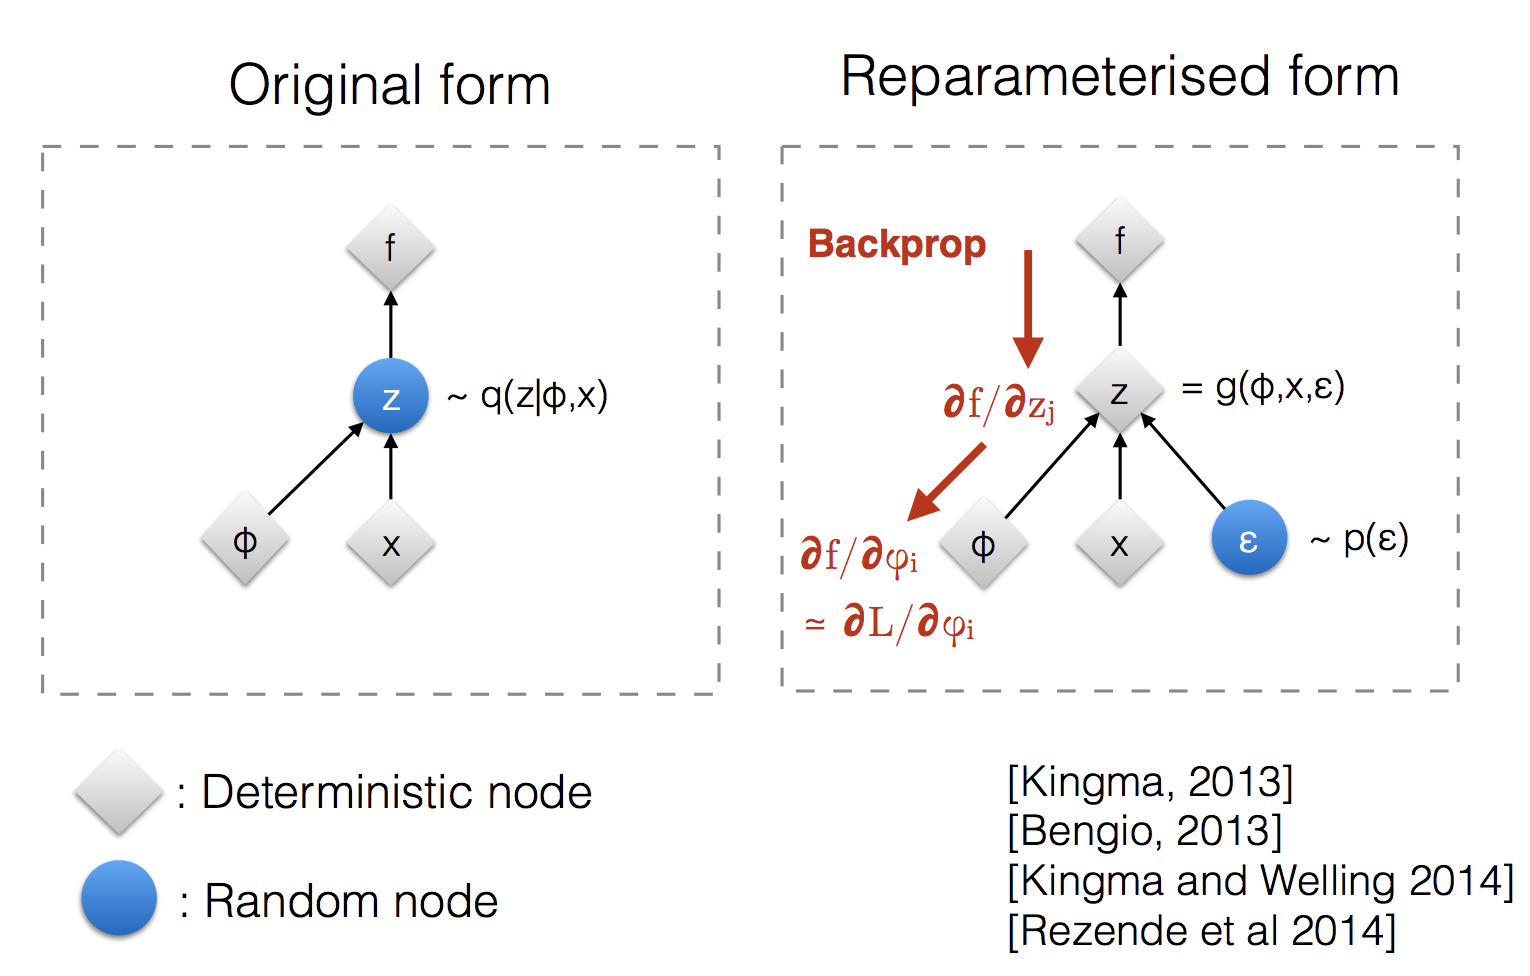
\includegraphics[height=0.45\textwidth]{figures/vae_reparameterization_trick}
    \caption{重参数方法示意图}\label{fig:vae_reparameterization_trick}
\end{figure}

式{\ref{eq:vae_max_elbo_approx}}中,变分自编码器使用重参数方法和蒙特卡洛方法,
对证据下界关于{$\phi$}和{$\theta$}同时进行优化。
训练完成后,即可直接从隐变量分布{$p(\bm{z})$}中进行采样,再经由解码器获得生成样本{$\bm{x}'$}。

层级变分自编码器是对变分自编码器的扩展{\cite{Luo2022UnderstandingDM}},
相比于变分自编码器,
层级变分自编码器可以有多层隐变量。
层级变分自编码器假设浅层隐变量由更深层的隐变量生成。
对于有{$T$}层隐变量的层级变分自编码器,
每一个隐变量都依赖于先前所有隐变量,
而其一个特例为马尔可夫层级变分自编码器。
马尔可夫层级变分自编码器中,
生成过程为马尔可夫链,
解码时每一个隐变量{$\bm{z}_{t}$}只依赖于之前一个隐变量{$\bm{z}_{t+1}$},
图{\ref{fig:markovian_hierarchical_variational_autoencoder}}为马尔可夫层级变分自编码器示意图。
\begin{figure}[ht]
    \centering
    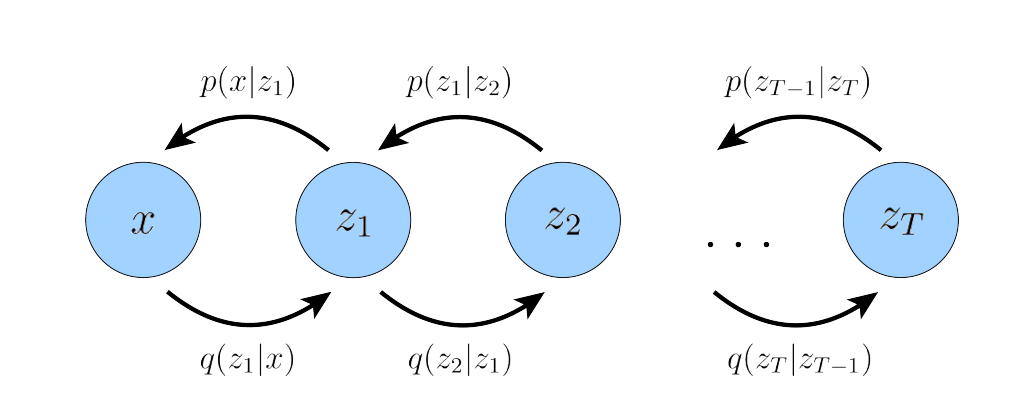
\includegraphics[width=0.8\textwidth]{figures/markovian_hierarchical_variational_autoencoder}
    \caption{马尔可夫层级变分自编码器示意图}\label{fig:markovian_hierarchical_variational_autoencoder}
\end{figure}

马尔可夫层级变分自编码器的联合概率分布可以表示为:
\begin{equation}
    \label{eq:mhvae_joint_distribution}
    p(\bm{x},\bm{z}_{1:T})=p(\bm{x}_{T})p_{\theta}(\bm{x}\mid \bm{z}_{1})\prod_{t=2}^{T}p_{\theta}(\bm{z}_{t-1}\mid\bm{z}_{t})
\end{equation}
其后验概率可以表为:
\begin{equation}
    \label{eq:mhvae_posterior}
    q_{\phi}(\bm{z}_{1:T} \mid \bm{x})=q_{\phi}(\bm{z}_{1}\mid \bm{x})\prod_{t=2}^{T}q_{\phi}(\bm{z}_{t}\mid\bm{z}_{t-1})
\end{equation}
证据下界可以扩展为:
\begin{align}
    \log p(\bm{x})
    & =\log \int p(\bm{x},\bm{z}_{1:T}) d\,z & \mbox{(根据式{\ref{eq:elbo_probability_of_x_with_integral}})} \\
    &=\log \int p(\bm{x},\bm{z}_{1:T})  \frac{q_{\phi}(\bm{z}_{1:T}\mid\bm{x})}{q_{\phi}(\bm{z}_{1:T}\mid\bm{x})} d\,z \\
    &=\log \int \frac{p(\bm{x},\bm{z}_{1:T}) q_{\phi}(\bm{z}_{1:T}\mid\bm{x})}{q_{\phi}(\bm{z}_{1:T}\mid\bm{x})} d\,z \\
    &=\log \int q_{\phi}(\bm{z}_{1:T}\mid\bm{x}) \frac{p(\bm{x},\bm{z}_{1:T}) }{q_{\phi}(\bm{z}_{1:T}\mid\bm{x})} d\,z \\
    &= \log \mathbb{E}_{q_{\phi}(\bm{z}_{1:T}|\bm{x})}\left[\frac{p(\bm{x},\bm{z}_{1:T})}{q_{\phi}(\bm{z}_{1:T}\mid\bm{x})}\right]  & \mbox{(根据期望定义式{\ref{eq:expection_continuous}})} \\
    &\geq \mathbb{E}_{q_{\phi}(\bm{z}_{1:T}|\bm{x})}\left[\log\frac{p(\bm{x},\bm{z}_{1:T})}{q_{\phi}(\bm{z}_{1:T}\mid\bm{x})}\right] & \mbox{(根据杰森不等式{\ref{eq:Jensen_ineuqality}})} \label{eq:mhvae_elbo_jensen_inequaality}
\end{align}
将式{\ref{eq:mhvae_joint_distribution}}与{\ref{eq:mhvae_posterior}}代入式{\ref{eq:mhvae_elbo_jensen_inequaality}}可得:
\begin{equation}
\label{eq:mhvae_elbo_with_substitution}
\mathbb{E}_{q_{\phi}(\bm{z}_{1:T}|\bm{x})}\left[\log\frac{p(\bm{x},\bm{z}_{1:T})}{q_{\phi}(\bm{z}_{1:T}\mid\bm{x})}\right] 
=\mathbb{E}_{q_{\phi}(\bm{z}_{1:T}|\bm{x})}\left[\log\frac
{p(\bm{z}_{T})p_{\theta}(\bm{x}\mid \bm{z}_{1})\prod_{t=2}^{T}p_{\theta}(\bm{z}_{t-1}\mid\bm{z}_{t})}
{q_{\phi}(\bm{z}_{1}\mid \bm{x})\prod_{t=2}^{T}q_{\phi}(\bm{z}_{t}\mid\bm{z}_{t-1})}
\right] 
\end{equation}

在扩散模型中,
式{\ref{eq:mhvae_elbo_with_substitution}}可以进一步分解更具有意义的成分。

此外,由于自编码器与降噪自编码器并不直接定义似然函数,
可以将自编码器和降噪自编码器视为隐式密度模型。
而变分自编码器由于使用证据下界对似然函数进行近似,
变分自编码器为近似估计的显示密度模型。



\subsubsection{扩散模型}
% 扩散模型历史
% 扩散模型结构
扩散模型,是近年来在生成图像领域最有影响力的模型之一。
在很多评价基准上,扩散模型已经取得了相比生成对抗网络更好的成绩。
就如2017——2020年生成对抗网络的流行,在2022年,扩散模型也被广泛地用于各项生成任务。

2015年,扩散模型被从物理学中借鉴引入至深度学习领域 {\cite{sohl2015deep}}。
2019年,基于分数的模型NCSN {\cite{song2019generative}}的提出,
以及2020年对基于分数的模型训练方法的改进,都为扩散模型的诞生打下了良好的基础。

扩散模型可以理解为加一定限制的马尔可夫层级变分自编码器:
\begin{enumerate}
    \item 隐变量维度与样本维度相同;
    \item 每一时间(层级)隐变量编码器的结构为预先定义的线性高斯模型,并非学习获得,即将前一层隐变量值作为高斯分布的均值;
    \item 隐变量编码器高斯分布的参数随着时间(层级)的变化而变化,且保证最终的隐变量分布为标准高斯分布。
\end{enumerate}
\begin{figure}[ht]
    \centering
    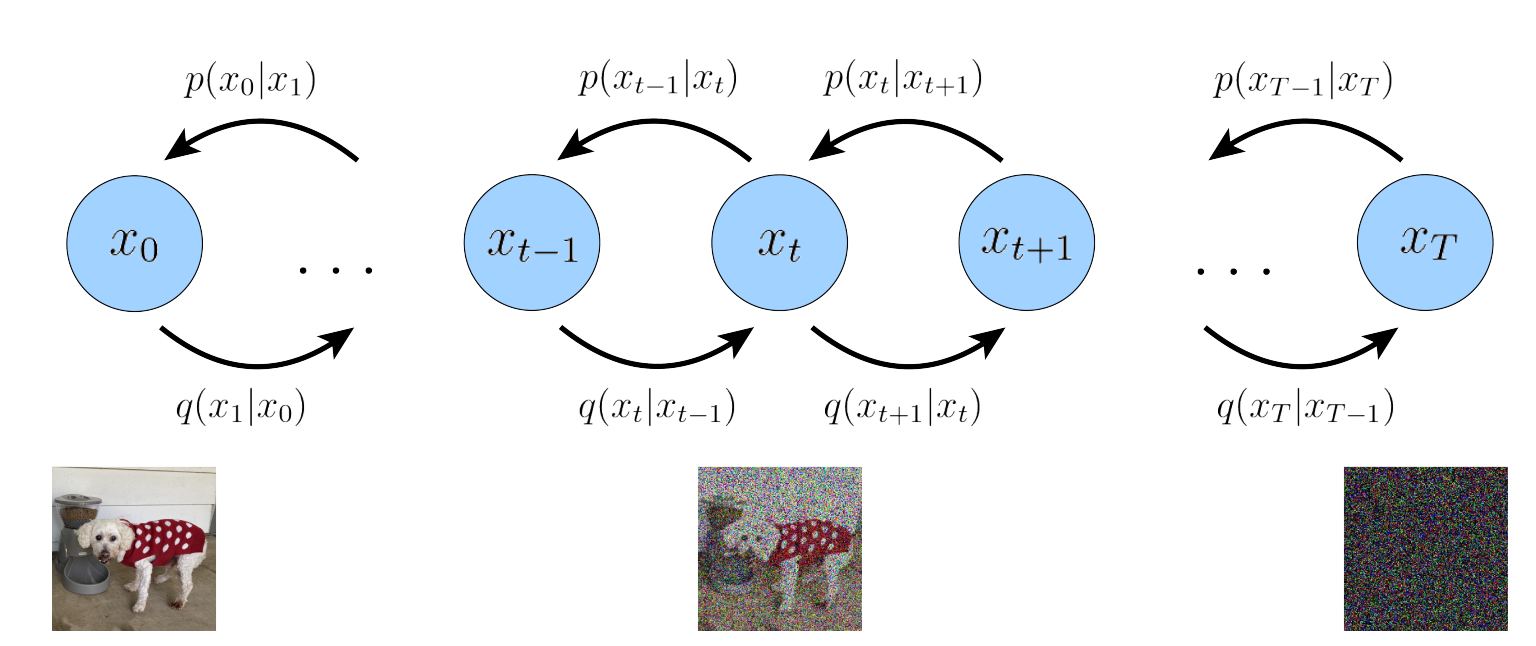
\includegraphics[width=\textwidth]{figures/diffusion_model}
    \caption{扩散模型示意图}\label{fig:diffusion_model}
\end{figure}

图{\ref{fig:diffusion_model}}为扩散模型示意图,
{$\bm{x}_{0}$}表示真实样本,如自然图像,
{$\bm{x}_{T}$}表示完全的高斯噪声,
{$\bm{x}_{t}$}表示真实样本{$\bm{x}_{0}$}添加噪声后所得的隐变量。
{$q(\bm{x}_{t}\mid \bm{x}_{t-1})$}为将前一状态作为均值的高斯分布。

由第一个假设,将真实样本和隐变量均由{$\bm{x}_{t}$}表示,
其中{$t=0$}表示真实样本,
{$t\in \left[1,T \right]$}表示相应的{$t$}层隐变量,
则扩散模型的后验与马尔可夫层级变分自编码器相似,
根据式{\ref{eq:mhvae_posterior}}得:
\begin{equation}
    \label{eq:diffusion_posterior}
    q(\bm{x}_{1:T} \mid \bm{x}_{0})=\prod_{t=1}^{T}q(\bm{x}_{t}\mid\bm{x}_{t-1})
\end{equation}

由第二个假设,编码器中隐变量服从以前一隐变量为均值的高斯分布,
与马尔可夫结构变分自编码器不同的是,
编码器在每一时间步{$t$}的结构并非学习获得,
而是预先设定的线性高斯模型,
均值和方差可以设为超参数{ {\cite{ho2020denoising}}},
或经学习获得{ {\cite{kingma2023variational}}}。
设高斯编码器均值为{$\bm{\mu}_{t}(\bm{x}_{t})=\sqrt{a_{t}}\bm{x}_{t-1}$},
方差为{$\bm{\Sigma}_{t}(\bm{x}_{t}) = (1-\alpha_t)\bm{I}$},
以使隐变量的方差大小相近。
为使模型更灵活,{$\alpha_t$}的值可以随着层级深度{$t$}的变化而变化。
编码转换过程可以表示为:
\begin{equation}
    \label{eq:diffusion_encoder}
    q(\bm{x}_{t}\mid \bm{x}_{t-1})=\mathcal{N}(\bm{x}_{t}; \sqrt{\alpha}_{t}(\bm{x}_{t-1}), (1-\alpha_t)\bm{I})
\end{equation}

由第三个假设,
预先定义或可学习获得的{$\alpha_t$}可以随着时间的变换而变化,
且最深层隐变量{$p(\bm{x}_T)$}的分布为标准高斯分布,
则马尔可夫层级变分自编码器的联合概率分布式{\ref{eq:mhvae_joint_distribution}}可以改写为:
\begin{equation}
    \label{eq:diffusion_joint_distribution}
    p(\bm{x}_{0:T})=p(\bm{x}_{T})\prod_{t=1}^{T}p_{\theta}(\bm{x}_{t-1}\mid\bm{x}_{t})
\end{equation}
式{\ref{eq:diffusion_joint_distribution}}中,
{$p(\bm{x}_T) = \mathcal{N}(\bm{x}_{T};\bm{0},\bm{I})$}。
假设三表明,扩散模型逐渐向图片添加噪声直至图片变为完全的高斯噪声,即如图{\ref{fig:diffusion_model}}所示。

相比于马尔可夫层级变分自编码器,
编码器分布{$q(\bm{x}_t\mid \bm{x}_{t-1})$}不再由参数{$\phi$}定义,
而完全服从预先定义了均值与方差的高斯分布。
因此,为能够生成新的样本点,
扩散模型更注重对条件概率{$p_{\theta}(\bm{x}_{t-1}\mid \bm{x}_{t})$}的学习。
对扩散模型优化后,
采样过程即为首先从高斯噪声{$p(\bm{x}_T)$}中采样,
随后连续地进行{$T$}次去噪变换{$p_{\theta}(\bm{x}_{t-1}\mid \bm{x}_{t})$},
最终获得新的样本点{$\bm{x}_{0}$}。

类比于层级变分自编码器,扩散模型可以通过最大化证据下界来优化,即:
\begin{align}
    \log p(\bm{x})
    &= \log \int p(\bm{x}_{0:T}) d\, \bm{x}_{1:T}
    \\ & = \log \int p(\bm{x}_{0:T}) \frac{q(\bm{x}_{1:T}\mid \bm{x}_{0})}{q(\bm{x}_{1:T}\mid \bm{x}_{0})} d\, \bm{x}_{1:T}
    \\ & = \log \int q(\bm{x}_{1:T}\mid \bm{x}_{0}) \frac{p(\bm{x}_{0:T}) }{q(\bm{x}_{1:T}\mid \bm{x}_{0})} d\, \bm{x}_{1:T}
    \\ & = \log \mathbb{E}_{q(\bm{x}_{1:T}\mid \bm{x}_{0})} \left[     \frac{p(\bm{x}_{0:T}) }{q(\bm{x}_{1:T}\mid \bm{x}_{0})}     \right]
    \\ & \geq  \mathbb{E}_{q(\bm{x}_{1:T}\mid \bm{x}_{0})} \left[   \log  \frac{p(\bm{x}_{0:T}) }{q(\bm{x}_{1:T}\mid \bm{x}_{0})}     \right] \label{eq:diffusion_elbo_origin}
    \\ & = \mathbb{E}_{q(\bm{x}_{1:T}\mid \bm{x}_{0})} \left[   \log  \frac{p(\bm{x}_{T}) \prod_{t=1}^{T}{p_{\theta}(\bm{x}_{t-1}\mid \bm{x}_{t})} }{\prod_{t=1}^{T}{q(\bm{x}_{t}\mid \bm{x}_{t-1})} }     \right]
    \\ & = \mathbb{E}_{q(\bm{x}_{1:T}\mid \bm{x}_{0})} \left[   \log  \frac{p(\bm{x}_{T})p_{\theta}(\bm{x}_{0} \mid \bm{x}_1) \prod_{t=2}^{T}{p_{\theta}(\bm{x}_{t-1}\mid \bm{x}_{t})} }{q(\bm{x}_{T}\mid \bm{x}_{T-1})\prod_{t=1}^{T-1}{q(\bm{x}_{t}\mid \bm{x}_{t-1})} }     \right]
    \\ & = \mathbb{E}_{q(\bm{x}_{1:T}\mid \bm{x}_{0})} \left[   \log  \frac{p(\bm{x}_{T})p_{\theta}(\bm{x}_{0} \mid \bm{x}_1) \prod_{t=1}^{T-1}{p_{\theta}(\bm{x}_{t}\mid \bm{x}_{t+1})} }{q(\bm{x}_{T}\mid \bm{x}_{T-1})\prod_{t=1}^{T-1}{q(\bm{x}_{t}\mid \bm{x}_{t-1})} }     \right]
    \\ & = \mathbb{E}_{q(\bm{x}_{1:T}\mid \bm{x}_{0})} \left[   \log  \frac{p(\bm{x}_{T})p_{\theta}(\bm{x}_{0} \mid \bm{x}_1)  }{q(\bm{x}_{T}\mid \bm{x}_{T-1})}     \right]
    + \mathbb{E}_{q(\bm{x}_{1:T}\mid \bm{x}_{0})} \left[   \log \prod_{t=1}^{T-1} {\frac{p_{\theta}(\bm{x}_{t}\mid \bm{x}_{t+1})} {q(\bm{x}_{t}\mid \bm{x}_{t-1})} }     \right]
    \\ & = \mathbb{E}_{q(\bm{x}_{1:T}\mid \bm{x}_{0})} \left[   \log  p(\bm{x}_{T})\right]
    + \mathbb{E}_{q(\bm{x}_{1:T}\mid \bm{x}_{0})} \left[   \log  \frac{p_{\theta}(\bm{x}_{0} \mid \bm{x}_1)  }{q(\bm{x}_{T}\mid \bm{x}_{T-1})}     \right]
    \nonumber \\ &\qquad+ \mathbb{E}_{q(\bm{x}_{1:T}\mid \bm{x}_{0})} \left[   \sum_{t=1}^{T-1} { \log \frac{p_{\theta}(\bm{x}_{t}\mid \bm{x}_{t+1})} {q(\bm{x}_{t}\mid \bm{x}_{t-1})} }     \right]
    \\ & = \mathbb{E}_{q(\bm{x}_{1:T}\mid \bm{x}_{0})} \left[   \log  p(\bm{x}_{T})\right]
    + \mathbb{E}_{q(\bm{x}_{1:T}\mid \bm{x}_{0})} \left[   \log  \frac{p_{\theta}(\bm{x}_{0} \mid \bm{x}_1)  }{q(\bm{x}_{T}\mid \bm{x}_{T-1})}     \right]
    \nonumber \\ &\qquad+ \sum_{t=1}^{T-1} \mathbb{E}_{q(\bm{x}_{1:T}\mid \bm{x}_{0})} \left[    { \log \frac{p_{\theta}(\bm{x}_{t}\mid \bm{x}_{t+1})} {q(\bm{x}_{t}\mid \bm{x}_{t-1})} }     \right]
    \\ & = \mathbb{E}_{q(\bm{x}_{1}\mid \bm{x}_{0})} \left[  \log  p_{\theta}(\bm{x}_{0}\mid \bm{x}_{1})\right]
    + \mathbb{E}_{q(\bm{x}_{T-1},\bm{x}_{T}\mid \bm{x}_{0})} \left[   \log  \frac{p_{\theta}(\bm{x}_{0} \mid \bm{x}_1)  }{q(\bm{x}_{T}\mid \bm{x}_{T-1})}     \right]
    \nonumber \\ & \qquad+ \sum_{t=1}^{T-1} \mathbb{E}_{q(\bm{x}_{T-1},\bm{x}_{t},\bm{x}_{t+1}\mid \bm{x}_{0})} \left[    { \log \frac{p_{\theta}(\bm{x}_{t}\mid \bm{x}_{t+1})} {q(\bm{x}_{t}\mid \bm{x}_{t-1})} }     \right]
    \\ & = \underbrace{\mathbb{E}_{q(\bm{x}_{1}\mid \bm{x}_{0})} \left[   \log  p_{\theta}(\bm{x}_{0}\mid \bm{x}_{1})\right]}_{\mbox{重构项}}
    - \underbrace{\mathbb{E}_{q(\bm{x}_{T-1}\mid \bm{x}_{0})}{\left[D_{KL}(q(\bm{x}_{T}\mid \bm{x}_{T-1}) \Vert p(\bm{x}_{T}) )\right]}}_{\mbox{先验匹配项}}
    \nonumber \\ & \qquad - \sum_{t=1}^{T-1} \underbrace{\mathbb{E}_{q(\bm{x}_{t-1},\bm{x}_{t+1}\mid \bm{x}_0)} \left[ D_{KL}( q(\bm{x}_{t}\mid\bm{x}_{t-1} )  \Vert  p_{\theta}(\bm{x}_{t}\mid \bm{x}_{t+1})   )  \right]    }_{\mbox{一致检验项}} \label{eq:diffusion_elbo}
\end{align}
式{\ref{eq:diffusion_elbo}}中:
\begin{itemize}
    \item {$\mathbb{E}_{q(\bm{x}_{1}\mid \bm{x}_{0})} \left[   \log  p_{\theta}(\bm{x}_{0}\mid \bm{x}_{1})\right]$}
项为重构项,是对样本点关于第一层隐变量的对数条件概率的预测,与一般变分自编码器式{\ref{eq:vae_elbo_dissect}}中的重构项类似,可由蒙特卡洛模拟近似计算与优化。
    \item {$\mathbb{E}_{q(\bm{x}_{T-1}\mid \bm{x}_{0})}{\left[D_{KL}(q(\bm{x}_{T}\mid \bm{x}_{T-1}) \Vert p(\bm{x}_{T}) )\right]}$}
项为先验匹配项,当最后一层隐变量的概率分布为高斯分布时达到最小,先验匹配项由于没有需要学习的参数,因此无需进行优化,
假设当{$T$}足够大,则最后一层隐变量的概率分布为高斯分布,先验匹配项的值为{$0$}。
    \item {$\mathbb{E}_{q(\bm{x}_{t-1},\bm{x}_{t+1}\mid \bm{x}_0)} \left[ D_{KL}( q(\bm{x}_{t}\mid\bm{x}_{t-1} )  \Vert  p_{\theta}(\bm{x}_{t}\mid \bm{x}_{t+1})   )  \right]     $}
项为一致检验项,一致检验项使扩散模型的前向过程和反向过程在{$\bm{x}_{t}$}保持一致,
即降噪过程获得的{$p_{\theta}(\bm{x}_{t}\mid \bm{x}_{t+1})$}应与高斯分布{$q(\bm{x}_{t}\mid \bm{x}_{t-1})$}尽可能一致。
\end{itemize}
\begin{figure}[ht]
    \centering
    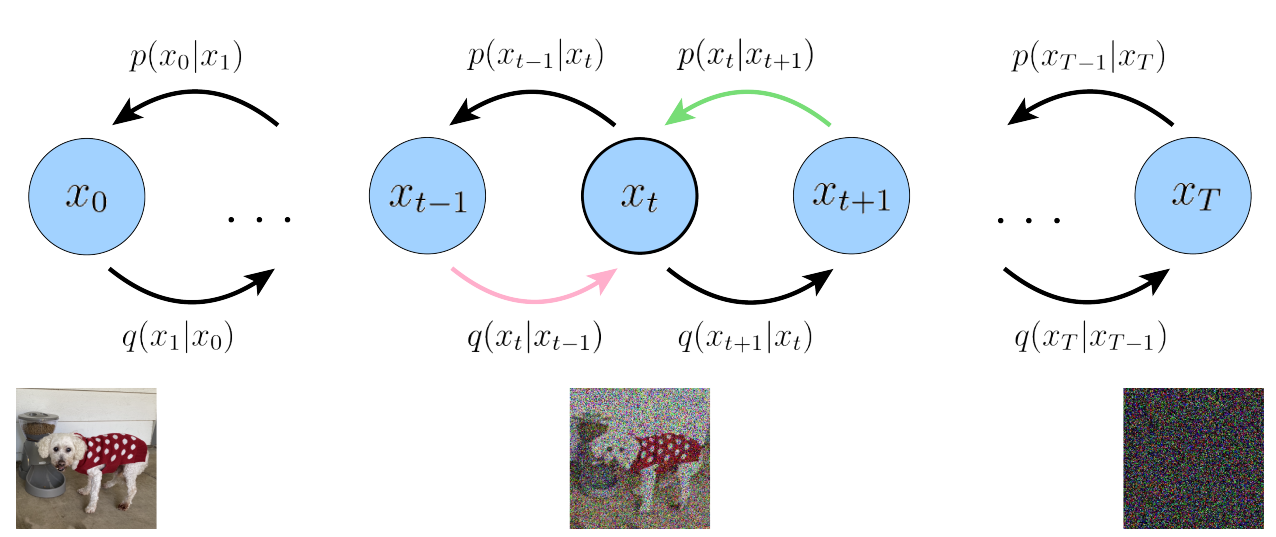
\includegraphics[width=\textwidth]{figures/diffusion_model_optimize_elbo}
    \caption{扩散模型证据下界一致检验项示意图}\label{fig:diffusion_model_optimize_elbo}
\end{figure}

图{\ref{fig:diffusion_model_optimize_elbo}}中,对于中间层隐变量{$\bm{x}_t$},
可以通过减小绿色箭头所代表的条件概率{$p(\bm{x}_{t}\mid \bm{x}_{t+1})$}与粉色箭头代表的高斯分布{$q(\bm{x}_{t}\mid \bm{x}_{t-1})$}的差异来优化,
由于需要对所有时间步骤{$t$}进行优化,扩散模型的优化时间取决于一致检验项。

式{\ref{eq:diffusion_elbo}}将证据下界分解为不同的期望项,
因此可以使用蒙特卡洛模拟来获得近似解,
但由于一致检验项在每个时间步计算关于两个随机变量{$\bm{x}_{t-1},\bm{x}_{t+1}$}的期望,
其蒙特卡洛估计的方差可能相比每个时间步只关于一个随机变量的项更高。
此外,由于需要对{$T-1$}步一致检验项进行求和,当{$T$}越大时,证据下界估计值的方差也越大。

由于马尔可夫性质,
{$\bm{x}_{t}$}不依赖于{$\bm{x}_{0}$},
可将编码过程改写为{$q(\bm{x}_{t}\mid \bm{x}_{t-1})=q(\bm{x}_{t}\mid \bm{x}_{t-1},\bm{x}_{0})$},
则根据贝叶斯定理可得:
\begin{equation}
    \label{eq:diffusion_rewrite_with_x_0}
    q(\bm{x}_{t}\mid \bm{x}_{t-1},\bm{x}_0)=\frac{q(\bm{x}_{t-1}\mid \bm{x}_{t},\bm{x}_0)q(\bm{x}_{t}\mid \bm{x}_0)}{q(\bm{x}_{t-1}\mid \bm{x}_0)}
\end{equation}
根据式{\ref{eq:diffusion_rewrite_with_x_0}},可由式{\ref{eq:diffusion_elbo_origin}}得:
\begin{align}
    &\log p(\bm{x})
    \\\geq &  \mathbb{E}_{q(\bm{x}_{1:T}\mid \bm{x}_0)} \left[ \log \frac{p(\bm{x}_{0:T})}{q(\bm{x}_{1:T}\mid \bm{x}_{0})}  \right]
    \\= &  \mathbb{E}_{q(\bm{x}_{1:T}\mid \bm{x}_0)} \left[ \log \frac{p(\bm{x}_{T})\prod_{t=1}^{T}{p_{\theta}(\bm{x}_{t-1}\mid \bm{x}_{t})}}{\prod_{t=1}^{T}q(\bm{x}_{t}\mid \bm{x}_{t-1})}  \right]
    \\= &  \mathbb{E}_{q(\bm{x}_{1:T}\mid \bm{x}_0)} \left[ \log \frac{p(\bm{x}_{T})p_{\theta}(\bm{x}_{0}\mid \bm{x}_{1})\prod_{t=2}^{T}{p_{\theta}(\bm{x}_{t-1}\mid \bm{x}_{t})}}{q(\bm{x}_{1}\mid \bm{x}_{0})\prod_{t=2}^{T}q(\bm{x}_{t}\mid \bm{x}_{t-1})}  \right]
    \\= &  \mathbb{E}_{q(\bm{x}_{1:T}\mid \bm{x}_0)} \left[ \log \frac{p(\bm{x}_{T})p_{\theta}(\bm{x}_{0}\mid \bm{x}_{1})\prod_{t=2}^{T}{p_{\theta}(\bm{x}_{t-1}\mid \bm{x}_{t})}}{q(\bm{x}_{1}\mid \bm{x}_{0})\prod_{t=2}^{T}q(\bm{x}_{t}\mid \bm{x}_{t-1},\bm{x}_{0})}  \right]
    \\= &  \mathbb{E}_{q(\bm{x}_{1:T}\mid \bm{x}_0)} \left[ \log \frac{p(\bm{x}_{T})p_{\theta}(\bm{x}_{0}\mid \bm{x}_{1})}{q(\bm{x}_{1}\mid \bm{x}_{0})} 
     + \log \prod_{t=2}^{T}\frac{p_{\theta}(\bm{x}_{t-1}\mid \bm{x}_{t})}{q(\bm{x}_{t}\mid \bm{x}_{t-1},\bm{x}_{0})} \right]
    \\= &  \mathbb{E}_{q(\bm{x}_{1:T}\mid \bm{x}_0)} \left[ \log \frac{p(\bm{x}_{T})p_{\theta}(\bm{x}_{0}\mid \bm{x}_{1})}{q(\bm{x}_{1}\mid \bm{x}_{0})} 
    + \log \prod_{t=2}^{T}\frac{p_{\theta}(\bm{x}_{t-1}\mid \bm{x}_{t})}{\frac{q(\bm{x}_{t-1}\mid \bm{x}_{t},\bm{x}_0)q(\bm{x}_{t}\mid \bm{x}_0)}{q(\bm{x}_{t-1}\mid \bm{x}_0)}} \right]
   \\= & \mathbb{E}_{q(\bm{x}_{1:T}\mid \bm{x}_0)} \left[ \log \frac{p(\bm{x}_{T})p_{\theta}(\bm{x}_{0}\mid \bm{x}_{1})}{q(\bm{x}_{1}\mid \bm{x}_{0})} 
   + \log \frac{q(\bm{x}_{1}\mid \bm{x}_{0})}{q(\bm{x}_{T}\mid \bm{x}_{0})}
   + \log \prod_{t=2}^{T}\frac{p_{\theta}(\bm{x}_{t-1}\mid \bm{x}_{t})}{q(\bm{x}_{t-1}\mid \bm{x}_{t},\bm{x}_0)} \right]
  \\= &  \mathbb{E}_{q(\bm{x}_{1:T}\mid \bm{x}_0)} \left[ \log \frac{p(\bm{x}_{T})p_{\theta}(\bm{x}_{0}\mid \bm{x}_{1})}{q(\bm{x}_{T}\mid \bm{x}_{0})} 
   + \sum_{t=2}^{T}\log \frac{p_{\theta}(\bm{x}_{t-1}\mid \bm{x}_{t})}{q(\bm{x}_{t-1}\mid \bm{x}_{t},\bm{x}_0)}\right]
   \\= & \mathbb{E}_{q(\bm{x}_{1:T}\mid \bm{x}_0)} \left[  \log p_{\theta}(\bm{x}_{0}\mid \bm{x}_{1}) \right]
   +  \mathbb{E}_{q(\bm{x}_{1:T}\mid \bm{x}_0)} \left[ \log \frac{p(\bm{x}_{T})}{q(\bm{x}_{T}\mid \bm{x}_{0})} \right]
   \nonumber \\ & \qquad+   \sum_{t=2}^{T} \mathbb{E}_{q(\bm{x}_{1:T}\mid \bm{x}_0)} \left[  \log \frac{p_{\theta}(\bm{x}_{t-1}\mid \bm{x}_{t})}{q(\bm{x}_{t-1}\mid \bm{x}_{t},\bm{x}_0)} \right]
   \\ &  = \mathbb{E}_{q(\bm{x}_{1}\mid \bm{x}_0)} \left[  \log p_{\theta}(\bm{x}_{0}\mid \bm{x}_{1}) \right]
   +  \mathbb{E}_{q(\bm{x}_{T}\mid \bm{x}_0)} \left[ \log \frac{p(\bm{x}_{T})}{q(\bm{x}_{T}\mid \bm{x}_{0})} \right]
   \nonumber \\ & \qquad+   \sum_{t=2}^{T} \mathbb{E}_{q(\bm{x}_{t},\bm{x}_{t-1}\mid \bm{x}_0)} \left[  \log \frac{p_{\theta}(\bm{x}_{t-1}\mid \bm{x}_{t})}{q(\bm{x}_{t-1}\mid \bm{x}_{t},\bm{x}_0)} \right]
   \\ &  = \underbrace{\mathbb{E}_{q(\bm{x}_{1}\mid \bm{x}_0)} \left[  \log p_{\theta}(\bm{x}_{0}\mid \bm{x}_{1}) \right]}_{\mbox{重构项}}
   - \underbrace{D_{KL}(q(\bm{x}_{T}\mid \bm{x}_{0}) \Vert p(\bm{x}_{T}))}_{\mbox{先验匹配项}}
   \nonumber \\ & \qquad - \sum_{t=2}^{T} \underbrace{\mathbb{E}_{q(\bm{x}_{t}\mid \bm{x}_0)} \left[ D_{KL}(q(\bm{x}_{t-1}\mid \bm{x}_{t},\bm{x}_0)\Vert p_{\theta}(\bm{x}_{t-1}\mid \bm{x}_{t}))  \right]}_{\mbox{降噪匹配项}} \label{eq:diffusion_elbo_expectation_single}
\end{align}

式{\ref{eq:diffusion_elbo_expectation_single}}相比式{\ref{eq:diffusion_elbo}},
每一项均为最多只关于一个随机变量的期望。
类比对式{\ref{eq:diffusion_elbo}}的解释,
式{\ref{eq:diffusion_elbo_expectation_single}}有如下解释:
\begin{itemize}
    \item {$\mathbb{E}_{q(\bm{x}_{1}\mid \bm{x}_0)} \left[  \log p_{\theta}(\bm{x}_{0}\mid \bm{x}_{1}) \right]$}
项为重构项,与变分自编码器证据下界中的重构项类似。可以蒙特卡洛模拟方法近似估计与优化。
\item {$D_{KL}(q(\bm{x}_{T}\mid \bm{x}_{0}) \Vert p(\bm{x}_{T}))$}项为先验匹配项,
表明不断添加噪声后的图像与高斯分布的匹配程度。
先验匹配项在扩散模型假设下为{$0$}。
\item {$ \mathbb{E}_{q(\bm{x}_{t}\mid \bm{x}_0)} \left[ D_{KL}(q(\bm{x}_{t-1}\mid \bm{x}_{t},\bm{x}_0)\Vert p_{\theta}(\bm{x}_{t-1}\mid \bm{x}_{t}))  \right] $ }
为降噪匹配项,
扩散模型用降噪变换{$p_{\theta}(\bm{x}_{t-1}\mid \bm{x}_{t})$}来近似真实降噪变换{$q(\bm{x}_{t-1}\mid \bm{x}_{t},\bm{x}_0)$}。
通过最小化降噪匹配项,
可以使两个降噪变换逐渐接近。
\end{itemize}
\begin{figure}[ht]
    \centering
    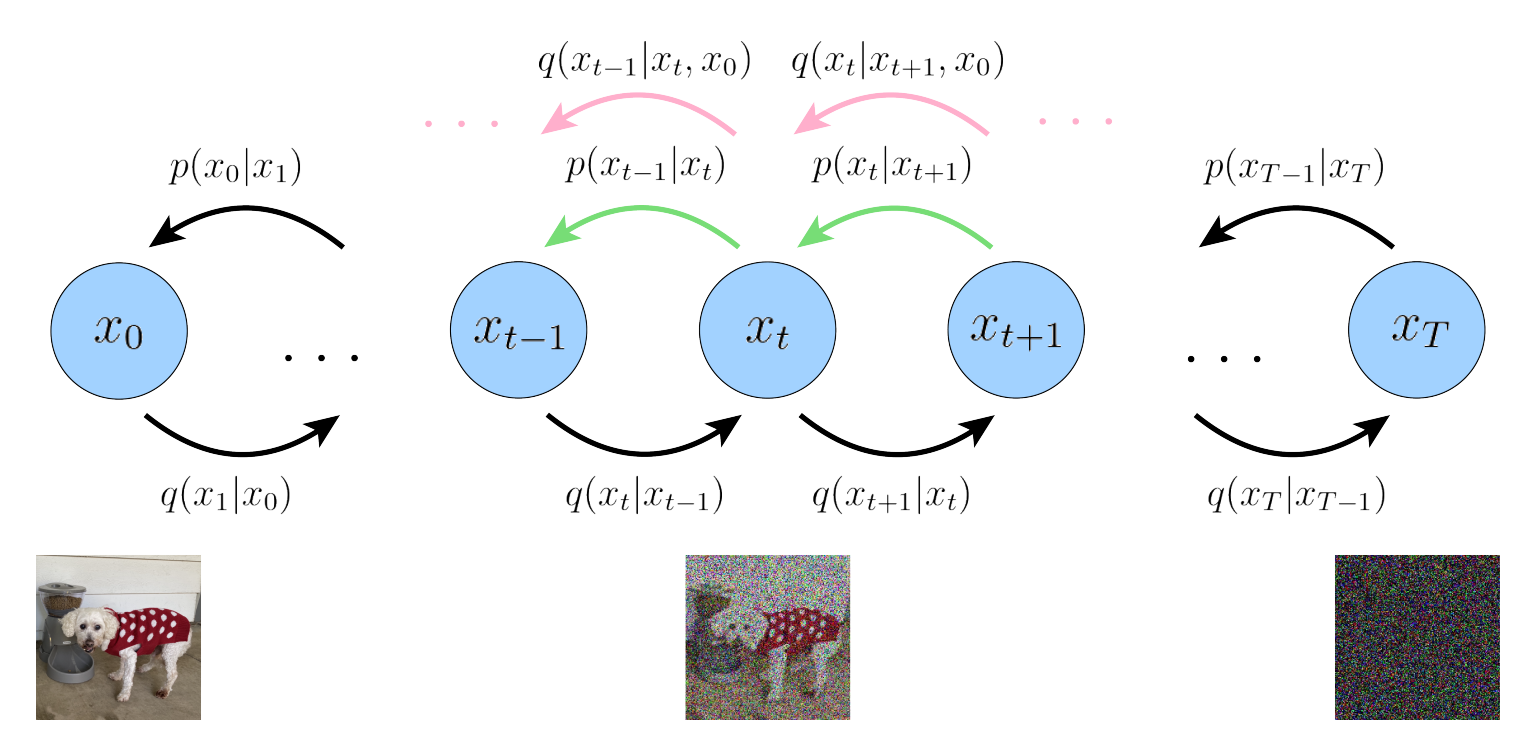
\includegraphics[width=\textwidth]{figures/diffusion_model_optimize_elbo_single_variable}
    \caption{扩散模型证据下界降噪匹配项单变量期望示意图}\label{fig:diffusion_model_optimize_elbo_single_variable}
\end{figure}

图{\ref{fig:diffusion_model_optimize_elbo_single_variable}}为使用式{\ref{eq:diffusion_elbo_expectation_single}}优化扩散模型示意图,
使用贝叶斯定理计算真实降噪过程{$q(\bm{x}_{t-1}\mid \bm{x}_{t},\bm{x}_0)$},
并计算其关于近似降噪过程{$p_{\theta}(\bm{x}_{t-1}\mid \bm{x}_{t})$}的KL散度,
即尽可能使绿色箭头所代表分布与粉色箭头所代表分布一致。

KL散度项{$D_{KL}(q(\bm{x}_{t-1}\mid \bm{x}_{t},\bm{x}_0)\Vert p_{\theta}(\bm{x}_{t-1}\mid \bm{x}_{t})) $}
由于需要同时对多个时间步的编码器进行学习,
难以进行最小化。
为使KL散度项更易优化,
根据贝叶斯定理有:
\begin{equation}
    \label{eq:diffusion_gaussion_transition_for_kl_divergence}
    q(\bm{x}_{t-1}\mid \bm{x}_{t},\bm{x}_0)=\frac{q(\bm{x}_{t}\mid \bm{x}_{t-1},\bm{x}_0) q(\bm{x}_{t-1}\mid \bm{x}_0)}{q(\bm{x}_{t}\mid \bm{x}_0) }
\end{equation}
根据式{\ref{eq:diffusion_encoder}},可得:
\begin{equation}
    \label{eq:diffusion_gaussion_transition_for_kl_divergence_likelihood}
    q(\bm{x}_{t}\mid \bm{x}_{t-1},\bm{x}_0)=q(\bm{x}_{t}\mid \bm{x}_{t-1})=\mathcal{N}(\bm{x}_{t}; \sqrt{\alpha}_{t}(\bm{x}_{t-1}), (1-\alpha_t)\bm{I})
\end{equation}
由于扩散模型编码器为线性高斯模型,
根据重参数方法,
对于{$\bm{x}_{t}\sim q(\bm{x}_{t},\bm{x}_{t-1})$}可得:
\begin{equation}
    \bm{x}_{t}=\sqrt{\alpha_{t}}\bm{x}_{t-1}+\sqrt{1-\alpha_{t}}\bm{\epsilon} \mbox{其中,} \epsilon \sim \mathcal{N}(\bm{\epsilon};\bm{0},\bm{I})
\end{equation}
对于{$\bm{x}_{t-1}\sim q(\bm{x}_{t-1},\bm{x}_{t-2})$}可得:
\begin{equation}
    \bm{x}_{t-1}=\sqrt{\alpha_{t-1}}\bm{x}_{t-2}+\sqrt{1-\alpha_{t-1}}\bm{\epsilon} \mbox{其中,} \epsilon \sim \mathcal{N}(\bm{\epsilon};\bm{0},\bm{I})
\end{equation}

可以使用重参数方法对{$q(\bm{x}_{t}\mid \bm{x}_{0})$}进行递归推导,
假设有{$2T$}个随机噪声变量{$\{\bm{\epsilon}_{t}^{*},\bm{\epsilon}_{t}\}_{t=0}^{T} \stackrel {iid} \sim \mathcal{N}(\bm{\epsilon;\bm{0},\bm{I}})$},
则对于任意采样{$\bm{x}_{t}\sim q(\bm{x}_{t}\mid \bm{x}_{0})$},有:
\begin{align}
    \bm{x}_{t}
    &=\sqrt{\alpha_{t}}\bm{x}_{t-1} +\sqrt{1-\alpha_{t}}\bm{\epsilon}_{t-1}^{*}
    \\ & = \sqrt{\alpha}_{t}(  \sqrt{\alpha}_{t-1} \bm{x}_{t-2} +\sqrt{1-\alpha_{t-1}}\bm{\epsilon}_{t-2}^{*}  ) +\sqrt{1-\alpha_{t}}\bm{\epsilon}_{t-1}^{*}
    \\ & = \sqrt{\alpha_{t}\alpha_{t-1}}\bm{x}_{t-2}  + \sqrt{\alpha_{t}-\alpha_{t}\alpha_{t-1}}\bm{\epsilon}_{t-2}^{*} +\sqrt{1-\alpha_{t}}\bm{\epsilon}_{t-1}^{*}
    \\ & = \sqrt{\alpha_{t}\alpha_{t-1}}\bm{x}_{t-2}  + \sqrt{\sqrt{{\alpha_{t}-\alpha_{t}\alpha_{t-1}}}^{2}+{\sqrt{1-\alpha_{t}}}^{2}}\bm{\epsilon}_{t-2} \mbox{\qquad 根据式{\ref{eq:sum_of_two_gaussian_distributions}}}
    \\ & = \sqrt{\alpha_{t}\alpha_{t-1}}\bm{x}_{t-2}  +\sqrt{\alpha_{t}-\alpha_{t}\alpha_{t-1} + 1-\alpha_{t}} \bm{\epsilon}_{t-2}
    \\ & =\sqrt{\alpha_{t}\alpha_{t-1}}\bm{x}_{t-2}  +\sqrt{1-\alpha_{t}\alpha_{t-1} } \bm{\epsilon}_{t-2}
    \\ & = \ldots
    \\ & = \sqrt{\prod_{i=1}^{t}\alpha_{i}}\bm{x}_{0}+ \sqrt{1- \prod_{i=1}^{t}\alpha_{i}}\bm{\epsilon}_{0}
    \\ & = \sqrt{\bar{\alpha}_{t}}\bm{x}_{0} +\sqrt{1- \bar{\alpha}_{t}}\bm{\epsilon}_{0}
    \\ & \sim \mathcal{N}(\bm{x}_{t}; \sqrt{\bar{\alpha}_{t}}\bm{x}_{0},(1- \bar{\alpha}_{t})\bm{I}) \label{eq:diffusion_x_t_gaussian_distribution}
\end{align}
与式{\ref{eq:diffusion_x_t_gaussian_distribution}}类似,有:
\begin{equation}
    \label{eq:diffusion_x_t_minux_1_gaussian_distribution}
    \bm{x}_{t-1} \sim \mathcal{N}(\bm{x}_{t-1}; \sqrt{\bar{\alpha}_{t-1}}\bm{x}_{0},(1- \bar{\alpha}_{t-1})\bm{I})
\end{equation}

由式{\ref{eq:diffusion_gaussion_transition_for_kl_divergence}}、
式{\ref{eq:diffusion_gaussion_transition_for_kl_divergence_likelihood}}、
式{\ref{eq:diffusion_x_t_gaussian_distribution}}和式{\ref{eq:diffusion_x_t_minux_1_gaussian_distribution}},
可得:
\begin{align}
    &q(\bm{x}_{t-1}\mid \bm{x}_{t},\bm{x}_0)
    \\ = &\frac{q(\bm{x}_{t}\mid \bm{x}_{t-1},\bm{x}_0) q(\bm{x}_{t-1}\mid \bm{x}_0)}{q(\bm{x}_{t}\mid \bm{x}_0) }
    \\  \propto & \exp \{ -\frac{1}{2}  \left[   \frac{{(\bm{x}_{t}-\sqrt{\alpha_{t}}\bm{x}_{t-1})}^{2}}{1-\alpha_{t}}
    +  \frac{{(\bm{x}_{t-1}-\sqrt{\bar{\alpha}_{t-1}}\bm{x}_{0})}^{2}}{1-\bar{\alpha}_{t-1}}
    - \frac{{(\bm{x}_{t}-\sqrt{\bar{\alpha}_{t}}\bm{x}_{0})}^{2}}{1-\bar{\alpha}_{t}}
     \right]  \}
    \\ = & \exp \{ -\frac{1}{2}  \left[ 
    \frac{-2 \sqrt{\alpha_{t}}\bm{x}_{t}\bm{x}_{t-1}+\alpha_{t}\bm{x}_{t-1}^{2}}{1-\alpha_{t}}
     +  \frac{{(\bm{x}_{t-1}^{2} -2\sqrt{\bar{\alpha}_{t-1}}\bm{x}_{t-1}\bm{x}_{0})}^{2}}{1-\bar{\alpha}_{t-1}}
     + C(\bm{x}_{t},\bm{x}_{0})
        \right]  \} \label{eq:diffusion_kl_divergence_q_with_c}
    \\  \propto & \exp \{ -\frac{1}{2}  \left[ 
        -\frac{2 \sqrt{\alpha_{t}}\bm{x}_{t}\bm{x}_{t-1}}{1-\alpha_{t}}
        +\frac{\alpha_{t}\bm{x}_{t-1}^{2}}{1-\alpha_{t}}
        + \frac{\bm{x}_{t-1}^{2} }{1-\bar{\alpha}_{t-1}}
        - \frac{2\sqrt{\bar{\alpha}_{t-1}}\bm{x}_{t-1}\bm{x}_{0}}{1-\bar{\alpha}_{t-1}}
         \right]  \}
    \\ = & \exp \{ -\frac{1}{2}  \left[ 
    \left(\frac{\alpha_{t}}{1-\alpha_{t}}+ \frac{1}{1-\bar{\alpha}_{t-1}}\right) \bm{x}_{t-1}^{2}
    -2\left(\frac{\sqrt{\alpha_{t}}\bm{x}_{t}}{1-\alpha_{t}}  + \frac{\sqrt{\bar{\alpha}_{t-1}}\bm{x}_{0}}{1-\bar{\alpha}_{t-1}}  \right)\bm{x}_{t-1}
        \right]  \}
    \\ = & \exp \{ -\frac{1}{2}  \left[ 
    \frac{\alpha_{t}(1-\bar{\alpha}_{t-1})+1-\alpha_{t}}{(1-\alpha_{t})(1-\bar{\alpha}_{t-1})} \bm{x}_{t-1}^{2}
    -2\left(\frac{\sqrt{\alpha_{t}}\bm{x}_{t}}{1-\alpha_{t}}  + \frac{\sqrt{\bar{\alpha}_{t-1}}\bm{x}_{0}}{1-\bar{\alpha}_{t-1}}  \right)\bm{x}_{t-1}
        \right]  \}
    \\ = & \exp \{ -\frac{1}{2}  \left[ 
    \frac{\alpha_{t}-\bar{\alpha}_{t}+1-\alpha_{t}}{(1-\alpha_{t})(1-\bar{\alpha}_{t-1})} \bm{x}_{t-1}^{2}
    -2\left(\frac{\sqrt{\alpha_{t}}\bm{x}_{t}}{1-\alpha_{t}}  + \frac{\sqrt{\bar{\alpha}_{t-1}}\bm{x}_{0}}{1-\bar{\alpha}_{t-1}}  \right)\bm{x}_{t-1}
        \right]  \}
    \\ = & \exp \{ -\frac{1}{2}  \left[ 
    \frac{1-\bar{\alpha}_{t}}{(1-\alpha_{t})(1-\bar{\alpha}_{t-1})} \bm{x}_{t-1}^{2}
    -2\left(\frac{\sqrt{\alpha_{t}}\bm{x}_{t}}{1-\alpha_{t}}  + \frac{\sqrt{\bar{\alpha}_{t-1}}\bm{x}_{0}}{1-\bar{\alpha}_{t-1}}  \right)\bm{x}_{t-1}
        \right]  \}
    \\ = & \exp \{ -\frac{1}{2} \left(    \frac{1-\bar{\alpha}_{t}}{(1-\alpha_{t})(1-\bar{\alpha}_{t-1})} \right) \left[ 
   \bm{x}_{t-1}^{2}
   -2\frac{\left(\frac{\sqrt{\alpha_{t}}\bm{x}_{t}}{1-\alpha_{t}}  + \frac{\sqrt{\bar{\alpha}_{t-1}}\bm{x}_{0}}{1-\bar{\alpha}_{t-1}}  \right)}{  \frac{1-\bar{\alpha}_{t}}{(1-\alpha_{t})(1-\bar{\alpha}_{t-1})}}\bm{x}_{t-1}
        \right]  \}
    \\ = & \exp \{ -\frac{1}{2} \left(    \frac{1-\bar{\alpha}_{t}}{(1-\alpha_{t})(1-\bar{\alpha}_{t-1})} \right)
    \nonumber \\ & \qquad \qquad \left[ 
   \bm{x}_{t-1}^{2}
   -2\frac{\left(\frac{\sqrt{\alpha_{t}}\bm{x}_{t}}{1-\alpha_{t}}  + \frac{\sqrt{\bar{\alpha}_{t-1}}\bm{x}_{0}}{1-\bar{\alpha}_{t-1}}  \right)(1-\alpha_{t})(1-\bar{\alpha}_{t-1})}{  1-\bar{\alpha}_{t}}\bm{x}_{t-1}
        \right]  \}
    \\ = & \exp \{ -\frac{1}{2} \left(    \frac{1}{\frac{(1-\alpha_{t})(1-\bar{\alpha}_{t-1})}{1-\bar{\alpha}_{t}}} \right) \left[ 
   \bm{x}_{t-1}^{2}
   -2\frac{\sqrt{\alpha_{t}}(1-\bar{\alpha}_{t-1})\bm{x}_{t} + \sqrt{\bar{\alpha}_{t-1}}(1-\alpha_{t})\bm{x}_{0}}{  1-\bar{\alpha}_{t}}\bm{x}_{t-1}
        \right]  \} \label{eq:diffusion_kl_divergence_q_distribution_no_complete_square}
    \\ \propto  & \mathcal{N}(\bm{x}_{t-1};
    \underbrace{\frac{\sqrt{\alpha_{t}}(1-\bar{\alpha}_{t-1})\bm{x}_{t} + \sqrt{\bar{\alpha}_{t-1}}(1-\alpha_{t})\bm{x}_{0}}{  1-\bar{\alpha}_{t}}}_{\mu_{q}(\bm{x}_{t},\bm{x}_{0})},
    \underbrace{\frac{(1-\alpha_{t})(1-\bar{\alpha}_{t-1})}{1-\bar{\alpha}_{t}}\bm{I}}_{\bm{\Sigma}_{q}(t)}) \label{eq:diffusion_kl_divergence_q_distribution}
\end{align}

式{\ref{eq:diffusion_kl_divergence_q_with_c}}中,{$C(\bm{x}_{t},\bm{x}_{0})$}为由{$\bm{x}_{t},\bm{x}_{0},\alpha$}组成的相对于{$\bm{x}_{t-1}$}的常数项,
可与式{\ref{eq:diffusion_kl_divergence_q_distribution_no_complete_square}}经过配方法式{\ref{eq:completing_the_square_method}},
获得式{\ref{eq:diffusion_kl_divergence_q_distribution}}。
即{$\bm{x}_{t-1} \sim q(\bm{x}_{t-1}\mid \bm{x}_{t},\bm{x}_{0})$}为正态分布,
均值{$\mu_{q}(\bm{x}_{t},\bm{x}_{0})$}为{$\bm{x}_{t},\bm{x}_{0}$}的函数,
方差{$\bm{\Sigma}_{q}(t)$}为{$\alpha$}的函数,
{$\alpha$}为已知的关于时间步的确定量,
可以为超参数或由神经网络学习获得。
根据式{\ref{eq:diffusion_kl_divergence_q_distribution}},
可得:
\begin{equation}
    \label{eq:diffusion_q_sigma}
    \Sigma_{q}(t)= \sigma_{q}^{2}(t)\bm{I}= \frac{(1-\alpha_{t})(1-\bar{\alpha}_{t-1})}{1-\bar{\alpha}_{t}}\bm{I}
\end{equation}

为使近似降噪转换{$p_{\theta}(\bm{x}_{t-1}\mid \bm{x}_{t})$}与真实降噪转换{$q(\bm{x}_{t-1}\mid \bm{x}_{t},\bm{x}_{0})$}更加接近,
可以使{$p_{\theta}(\bm{x}_{t-1}\mid \bm{x}_{t})$}服从高斯分布。
此外,由于{$\alpha$}在转换过程中为固定值,
可以令近似降噪转换的方差与真实降噪转换的方差相同,即{$\bm{\Sigma}_{q}(t)= \sigma_{q}^{2}(t)\bm{I}$}。
而对于高斯分布的均值,由于真实降噪转换的高斯分布均值{$\mu_{q}(\bm{x}_{t},\bm{x}_{0})$}为{$\bm{x}_{t},\bm{x}_{0}$}的函数,
近似降噪转换{$p_{\theta}(\bm{x}_{t-1}\mid \bm{x}_{t})$}却不含有{$\bm{x}_{0}$},
可将近似降噪转换高斯分布的均值设为{$\bm{\mu}_{\theta}(\bm{x}_{t},t)$}。

根据两高斯分布KL散度计算式{\ref{eq:kl_divergence_of_two_gaussian}},
由于近似降噪转换的方差与真实降噪转换的方差相同,
最小化KL散度即转换为最小化两分布的均值,即:
\begin{align}
    &\argmin_{\theta} D_{KL}(q(\bm{x}_{t-1}\mid \bm{x}_{t},\bm{x}_{0}) \Vert p_{\theta}(\bm{x}_{t-1}\mid \bm{x}_{t})  )
    \\=& \argmin_{\theta}  D_{KL}(\mathcal{N}(\bm{x}_{t-1};\bm{\mu}_{q},\bm{\Sigma}_{q}(t))\Vert \mathcal{N}(\bm{x}_{t-1};\bm{\mu}_{\theta},\bm{\Sigma}_{q}(t)))
    \\=& \argmin_{\theta}  \frac{1}{2}\left[
        \log \frac{\left|  \bm{\Sigma}_{q}(t) \right|}{\left|  \bm{\Sigma}_{q}(t) \right|}
        - d
        +tr({\bm{\Sigma}_{q}(t)}^{-1}\bm{\Sigma}_{q}(t))
        +{(\bm{\mu}_{\theta}-\bm{\mu}_{q})}^{\intercal}{\bm{\Sigma}_{q}(t)}^{-1}(\bm{\mu}_{\theta}-\bm{\mu}_{q})
    \right]
    \\=& \argmin_{\theta}  \frac{1}{2}\left[\log 1 -d +d + {(\bm{\mu}_{\theta}-\bm{\mu}_{q})}^{\intercal}{\bm{\Sigma}_{q}(t)}^{-1}(\bm{\mu}_{\theta}-\bm{\mu}_{q})\right]
    \\=& \argmin_{\theta}  \frac{1}{2}\left[{(\bm{\mu}_{\theta}-\bm{\mu}_{q})}^{\intercal}{\bm{\Sigma}_{q}(t)}^{-1}(\bm{\mu}_{\theta}-\bm{\mu}_{q})\right]
    \\=& \argmin_{\theta}  \frac{1}{2}\left[{(\bm{\mu}_{\theta}-\bm{\mu}_{q})}^{\intercal}{\sigma_{q}^{2}(t)\bm{I}}^{-1}(\bm{\mu}_{\theta}-\bm{\mu}_{q})\right]
    \\=& \argmin_{\theta}  \frac{1}{2(\sigma_{q}^{2}(t))}\left[ {\Vert \bm{\mu}_{\theta}-\bm{\mu}_{q} \Vert}_{2}^{2}  \right] \label{eq:diffusion_kl_divergence_two_gaussian_mu}
\end{align}

式{\ref{eq:diffusion_kl_divergence_two_gaussian_mu}}中,
{$\bm{\mu}_{q}$}为{$\bm{\mu}_{q}(\bm{x}_{t},\bm{x}_{0})$}的缩写,
{$\bm{\mu}_{\theta}$}为{$\bm{\mu}_{\theta}(\bm{x}_{t},t)$}的缩写。
由式{\ref{eq:diffusion_kl_divergence_q_distribution}},真实降噪转换分布的均值为:
\begin{equation}
    \label{diffusion_mu_}
    \bm{\mu}_{q}(\bm{x}_{t},\bm{x}_{0})=\frac{\alpha_{t}(1-\bar{\alpha}_{t-1})\bm{x}_{t} + \sqrt{\bar{\alpha}_{t-1}}1-\alpha_{t}\bm{x}_{0}}{  1-\bar{\alpha}_{t}}
\end{equation}

为使近似降噪转换的均值{$\bm{\mu}_{\theta}(\bm{x}_{t},t)$}与真实降噪转换的均值{$\bm{\mu}_{q}(\bm{x}_{t},\bm{x}_{0})$}的均值尽可能一致,
由于近似降噪转换的均值{$\bm{\mu}_{\theta}(\bm{x}_{t},t)$}也包含{$\bm{x}_{t}$},可令两均值具有相似形式,即:
\begin{equation}
    \label{eq:diffusion_mu_theta}
    \bm{\mu}_{\theta}(\bm{x}_{t},t)=\frac{\alpha_{t}(1-\bar{\alpha}_{t-1})\bm{x}_{t} + \sqrt{\bar{\alpha}_{t-1}}1-\alpha_{t}\hat{\bm{x}}_{\theta}(\bm{x}_{t},t)}{  1-\bar{\alpha}_{t}}
\end{equation}

式{\ref{eq:diffusion_mu_theta}}中,
{$\hat{\bm{x}}_{\theta}(\bm{x}_{t},t)$}为由噪声图像{$\bm{x}_{t}$}和时间索引{$t$}预测原始样本{$\bm{x}_{0}$}的神经网络。
则优化问题可转化为:
\begin{align}
    &\argmin_{\theta} D_{KL}(q(\bm{x}_{t-1}\mid \bm{x}_{t},\bm{x}_{0}) \Vert p_{\theta}(\bm{x}_{t-1}\mid \bm{x}_{t})  )
    \\=& \argmin_{\theta}  D_{KL}(\mathcal{N}(\bm{x}_{t-1};\bm{\mu}_{q},\bm{\Sigma}_{q}(t))\Vert \mathcal{N}(\bm{x}_{t-1};\bm{\mu}_{\theta},\bm{\Sigma}_{q}(t)))
    \\=& \argmin_{\theta}  \frac{1}{2(\sigma_{q}^{2}(t))}\left[ {\Vert \bm{\mu}_{\theta}-\bm{\mu}_{q} \Vert}_{2}^{2}  \right] 
    \\=& \argmin_{\theta}  \frac{1}{2(\sigma_{q}^{2}(t))}\left[ \left\Vert 
    \frac{\alpha_{t}(1-\bar{\alpha}_{t-1})\bm{x}_{t} + \sqrt{\bar{\alpha}_{t-1}}1-\alpha_{t}\bm{x}_{0}}{  1-\bar{\alpha}_{t}}
    \right. \right. \\ & \qquad \qquad \left. \left. -\frac{\alpha_{t}(1-\bar{\alpha}_{t-1})\bm{x}_{t} + \sqrt{\bar{\alpha}_{t-1}}1-\alpha_{t}\hat{\bm{x}}_{\theta}(\bm{x}_{t},t)}{  1-\bar{\alpha}_{t}}
    \right\Vert_{2}^{2} \right]
    \\=& \argmin_{\theta}  \frac{1}{2(\sigma_{q}^{2}(t))}\left[ {\left\Vert 
    \frac{ \sqrt{\bar{\alpha}_{t-1}}(1-\alpha_{t})\hat{\bm{x}}_{\theta}(\bm{x}_{t}, t)}{  1-\bar{\alpha}_{t}}
    -\frac{\sqrt{\bar{\alpha}_{t-1}}1-\alpha_{t}\bm{x}_{0}}{  1-\bar{\alpha}_{t}}
    \right\Vert}_{2}^{2} \right]
    \\=& \argmin_{\theta}  \frac{1}{2(\sigma_{q}^{2}(t))}\left[ {\left\Vert 
    \frac{ \sqrt{\bar{\alpha}_{t-1}}(1-\alpha_{t})}{  1-\bar{\alpha}_{t}}
    (\hat{\bm{x}}_{\theta}(\bm{x}_{t}, t)-\bm{x}_{0})
    \right\Vert}_{2}^{2} \right]
    \\=& \argmin_{\theta}  \frac{1}{2(\sigma_{q}^{2}(t))}
    \frac{\bar{\alpha}_{t-1}{(1-\alpha_{t})}^{2}}{{ 1-\bar{\alpha}_{t}}^{2}}\left[ {\left\Vert
    \hat{\bm{x}}_{\theta}(\bm{x}_{t}, t)-\bm{x}_{0}
    \right\Vert}_{2}^{2}\right] \label{eq:diffusion_optimize}
\end{align}

由式{\ref{eq:diffusion_optimize}},对扩散模型的优化可以转化为对神经网络的训练,
该神经网络可以从任意时刻噪声图像来预测真实样本。
此外,对式{\ref{eq:diffusion_elbo_expectation_single}}中的降噪匹配求和项,
可以通过最小化所有时刻的期望{$\eta$} 来近似,即:
\begin{equation}
    \label{eq:diffusion_minimize_expectation_over_all_timesteps_for_sum_of_denoising_Matching}
    \argmin_{\theta}\mathbb{E}_{t\sim U\{2,T\}}\left[
         \mathbb{E}_{q(\bm{x}_{t}\mid \bm{x}_0)} \left[ D_{KL}(q(\bm{x}_{t-1}\mid \bm{x}_{t},\bm{x}_0)\Vert p_{\theta}(\bm{x}_{t-1}\mid \bm{x}_{t}))  \right]
    \right]
\end{equation}

噪声参数{$\alpha_{t}$}可设置为超参数,也可参与训练学习获得。
可以使用以{$\eta$}为参数的神经网络{$\hat{\alpha}_{\bm{\eta}}(t)$}来获得{$\alpha_{t}$},
但由于每个时间步{$t$}都需计算{$\alpha_{t}$},效率较低,
可将式{\ref{eq:diffusion_q_sigma}}代入式{\ref{eq:diffusion_optimize}},
可得:
\begin{align}
    &\frac{1}{2(\sigma_{q}^{2}(t))}
    \frac{\bar{\alpha}_{t-1}{(1-\alpha_{t})}^{2}}{{ 1-\bar{\alpha}_{t}}^{2}}\left[ {\left\Vert
    \hat{\bm{x}}_{\theta}(\bm{x}_{t}, t)-\bm{x}_{0}
    \right\Vert}_{2}^{2}\right]
    \\ = & \frac{1}{2\frac{(1-\alpha_{t})(1-\bar{\alpha}_{t-1})}{1-\bar{\alpha}_{t}}}
    \frac{\bar{\alpha}_{t-1}{(1-\alpha_{t})}^{2}}{{ 1-\bar{\alpha}_{t}}^{2}}\left[ {\left\Vert
    \hat{\bm{x}}_{\theta}(\bm{x}_{t}, t)-\bm{x}_{0}
    \right\Vert}_{2}^{2}\right]
    \\ = & \frac{1}{2}\frac{1-\bar{\alpha}_{t}}{(1-\alpha_{t})(1-\bar{\alpha}_{t-1})}
    \frac{\bar{\alpha}_{t-1}{(1-\alpha_{t})}^{2}}{{ 1-\bar{\alpha}_{t}}^{2}}\left[ {\left\Vert
    \hat{\bm{x}}_{\theta}(\bm{x}_{t}, t)-\bm{x}_{0}
    \right\Vert}_{2}^{2}\right]
    \\ = & \frac{1}{2}
    \frac{\bar{\alpha}_{t-1}(1-\alpha_{t})}{(1-\bar{\alpha}_{t-1})(1-\bar{\alpha}_{t})}
    \left[ {\left\Vert
    \hat{\bm{x}}_{\theta}(\bm{x}_{t}, t)-\bm{x}_{0}
    \right\Vert}_{2}^{2}\right]
    \\ = & \frac{1}{2}
    \frac{\bar{\alpha}_{t-1}-\bar{\alpha}_{t}}{(1-\bar{\alpha}_{t-1})(1-\bar{\alpha}_{t})}
    \left[ {\left\Vert
    \hat{\bm{x}}_{\theta}(\bm{x}_{t}, t)-\bm{x}_{0}
    \right\Vert}_{2}^{2}\right]
    \\ = & \frac{1}{2}
    \frac{\bar{\alpha}_{t-1}
    -\bar{\alpha}_{t}\bar{\alpha}_{t-1}+\bar{\alpha}_{t}\bar{\alpha}_{t-1}
    -\bar{\alpha}_{t}}
    {(1-\bar{\alpha}_{t-1})(1-\bar{\alpha}_{t})}
    \left[ {\left\Vert
    \hat{\bm{x}}_{\theta}(\bm{x}_{t}, t)-\bm{x}_{0}
    \right\Vert}_{2}^{2}\right]
    \\ = & \frac{1}{2}
    \frac{\bar{\alpha}_{t-1}(1-\bar{\alpha}_{t})-\bar{\alpha}_{t}(1-\bar{\alpha}_{t-1})}
    {(1-\bar{\alpha}_{t-1})(1-\bar{\alpha}_{t})}
    \left[ {\left\Vert
    \hat{\bm{x}}_{\theta}(\bm{x}_{t}, t)-\bm{x}_{0}
    \right\Vert}_{2}^{2}\right]
    \\ = & \frac{1}{2}\left(
        \frac{\bar{\alpha}_{t-1}(1-\bar{\alpha}_{t})}{(1-\bar{\alpha}_{t-1})(1-\bar{\alpha}_{t})}
        -\frac{\bar{\alpha}_{t}(1-\bar{\alpha}_{t-1})}{(1-\bar{\alpha}_{t-1})(1-\bar{\alpha}_{t})}
    \right)
    \left[ {\left\Vert
    \hat{\bm{x}}_{\theta}(\bm{x}_{t}, t)-\bm{x}_{0}
    \right\Vert}_{2}^{2}\right]
    \\ = & \frac{1}{2}\left(
        \frac{\bar{\alpha}_{t-1}}{1-\bar{\alpha}_{t-1}}
        -\frac{\bar{\alpha}_{t}}{1-\bar{\alpha}_{t}}
    \right)
    \left[ {\left\Vert
    \hat{\bm{x}}_{\theta}(\bm{x}_{t}, t)-\bm{x}_{0}
    \right\Vert}_{2}^{2}\right] \label{eq:diffusion_learning_diffusion_noise_parameters}
\end{align}

根据式{\ref{eq:diffusion_x_t_gaussian_distribution}},
{$q(\bm{x}_{t}\mid \bm{x}_{0})$}为服从高斯分布{$\mathcal{N}(\bm{x}_{t}; \sqrt{\bar{\alpha}_{t}}\bm{x}_{0},(1- \bar{\alpha}_{t})\bm{I})$},
则根据信噪比定义式{\ref{eq:signal_to_noise_ratio}}可得:
\begin{equation}
    \label{eq:diffusion_snr}
    SNR(t)=\frac{\bar{\alpha}_{t}}{1-\bar{\alpha}_{t}}
\end{equation}

根据式{\ref{eq:diffusion_snr}}可将式{\ref{eq:diffusion_learning_diffusion_noise_parameters}}改写为:
\begin{align}
    &\frac{1}{2(\sigma_{q}^{2}(t))}
    \frac{\bar{\alpha}_{t-1}{(1-\alpha_{t})}^{2}}{{ 1-\bar{\alpha}_{t}}^{2}}\left[ {\left\Vert
    \hat{\bm{x}}_{\theta}(\bm{x}_{t}, t)-\bm{x}_{0}
    \right\Vert}_{2}^{2}\right]
    \\ = &  \frac{1}{2}\left(
        \frac{\bar{\alpha}_{t-1}}{1-\bar{\alpha}_{t-1}}
        -\frac{\bar{\alpha}_{t}}{1-\bar{\alpha}_{t}}
    \right)
    \left[ {\left\Vert
    \hat{\bm{x}}_{\theta}(\bm{x}_{t}, t)-\bm{x}_{0}
    \right\Vert}_{2}^{2}\right] 
    \\ = &  \frac{1}{2}\left(
        SNR(t-1)-SNR(t)
    \right)
    \left[ {\left\Vert
    \hat{\bm{x}}_{\theta}(\bm{x}_{t}, t)-\bm{x}_{0}
    \right\Vert}_{2}^{2}\right] \label{eq:diffusion_learning_difufsion_noise_parameters_snr}
\end{align}

根据信噪比定义,信噪比越高,则包含更多的信息,信噪比越低,则噪声越多。
扩散模型的信噪比随着时间步{$t$}的增加而单调减小,
即{$\bm{x}_{t}$}随着时间推移而逐渐包含更多的噪声,
直至在{$t=T$}时变为标准高斯分布。

为简化式{\ref{eq:diffusion_learning_difufsion_noise_parameters_snr}},
可使用神经网络来模拟任意时间的信噪比,并与扩散模型同时训练。即:
\begin{equation}
    \label{eq:diffusion_snr_nn}
    SNR(t)=\exp(-\omega_{\bm{\eta}}(t))
\end{equation}

式{\ref{eq:diffusion_snr_nn}}中,
{$\omega_{\bm{\eta}}(t)$}为单调递增函数,
{$-\omega_{\bm{\eta}}(t)$}为单调递减函数,
进行指数化以使信噪比为正数。
此时,使用神经网络模拟任意时间信噪比,式{\ref{eq:diffusion_minimize_expectation_over_all_timesteps_for_sum_of_denoising_Matching}}需要同时对{$\bm{\eta}$}进行优化。

此外,由式{\ref{eq:diffusion_snr}}、式{\ref{eq:diffusion_snr_nn}}和式{\ref{eq:sigmoid_function}},
可得:
\begin{align}
    \frac{\bar{\alpha}_{t}}{1-\bar{\alpha}_{t}} & =\exp(-\omega_{\bm{\eta}}(t)) \\
    \bar{\alpha}_{t} & = sigmoid(-\omega_{\bm{\eta}}(t)) \label{eq:diffusion_bar_alpha_t}\\
    1-\bar{\alpha}_{t} & = sigmoid(\omega_{\bm{\eta}}(t)) \label{eq:diffusion_bar_1_minux_bar_alpha_t}
\end{align}

式{\ref{eq:diffusion_bar_alpha_t}}和式{\ref{eq:diffusion_bar_1_minux_bar_alpha_t}}可用于
式{\ref{eq:diffusion_kl_divergence_q_distribution_no_complete_square}}中使用重参数方法从原始样本{$\bm{x}_{0}$}生成任意时刻添加噪声后的图像{$\bm{x}_{t}$}。



%%%%%%%%%%%%%%%%%%%%%%%%%%%%%%%%%%%%%%%%%%%%%%%%%%%%%%%%%%%%%%%%%%%%%%%DIFFUSIONDIFFUSION





\section{隐式密度模型}\label{section:implicit_density_model}
隐式密度模型不定义概率密度函数{$p_{model}(\bm{x};\bm{\theta})$},
不通过最大化似然函数来训练,
而通过其他方式与实际概率密度函数{$p_{data}$}进行交互。
\subsection{生成对抗网络}
生成对抗网络可以视为根据博弈论设计的一场游戏,
包含两个机器学习模型,
机器学习模型通常采用神经网络。

其中一个神经网络为生成器,
其隐式地确定了概率分布{$p_{model}$},
生成器不需要对概率分布{$p_{model}$}进行评估。
根据一个先验分布{$p(\bm{z})$}以及生成函数方程{$G(\bm{z};\theta^{(G)})$},
生成器可以从概率分布{$p_{model}$}中采样,
其中可学习参数{$\theta^{(G)}$}确定了生成器在博弈中采取的策略,
先验分布{$p(\bm{z})$}经常为相对而言无特殊结构的分布,
比如高维高斯分布或超立方体均匀分布,
从这类分布中采样的{$\bm{z}$}为随机噪声。
生成器的主要任务是通过学习将随机噪声{$\bm{z}$}转化为能够以假乱真的样本。

另一个神经网络为辨别器,
辨别器可以通过辨别函数{$D(\bm{x};\bm{\theta}^{(D)})$},
判断一个样本{$x$}是从训练集中采样的真实样本或是由生成器生成的伪造样本。

在生成对抗网络游戏中,每一个玩家都有其本身的损失函数,
生成器的损失函数为{$J^{G}(\bm{\theta}^{(G)},\bm{\theta}^{(D)})$},
辨别器的损失函数为{$J^{D}(\bm{\theta}^{(G)},\bm{\theta}^{(D)})$}。
每一个玩家都希望能够最小化其损失函数。
辨别器的损失函数使其能够更好地辨别一个样本是真实样本还是伪造样本,
生成器的损失函数使其能够制造出可以迷惑辨别器的伪造样本,
使辨别器将伪造样本误认为真实样本。


生成对抗网络可以形象的表示成警察和造假者的博弈,
造假者尝试制造假币,
而警察在尽力逮捕造假者的同时,
还要保证正规货币的流通。
随着警察和造假者的博弈,
造假者的“造假”能力逐渐提高,
直至警察无法分辨。
对于生成对抗网络的训练过程,
可以比喻为造假者在警察中有内线,
其可以向造假者提供警方辨别真假的方法,
以让造假者制造更具有迷惑性的假币。



\begin{figure}[ht]
    \centering
    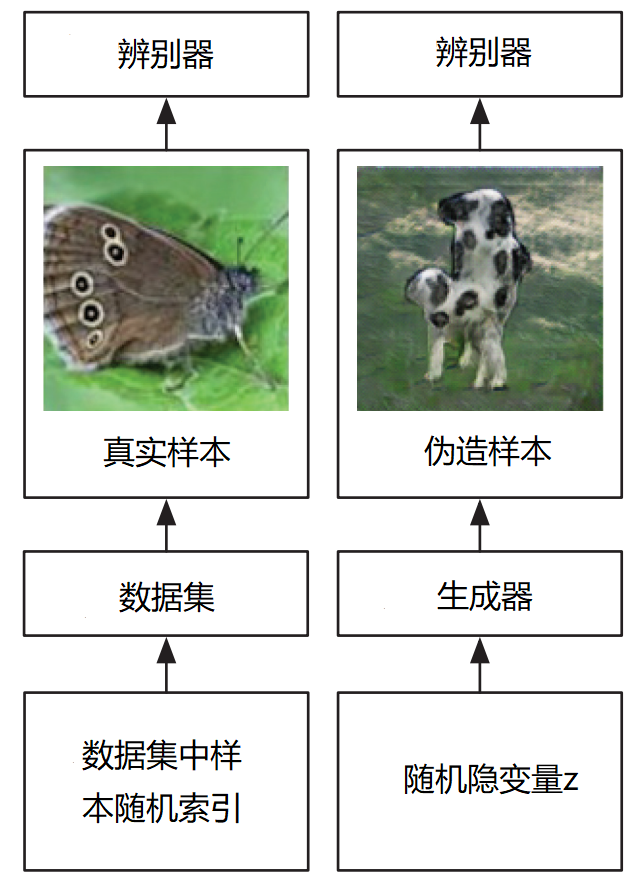
\includegraphics[height=0.5\textheight]{figures/gan_training}
    \caption{生成对抗网络训练过程}\label{fig:gan_training}
\end{figure}

图{\ref{fig:gan_training}}为生成对抗网络训练过程,
生成对抗网络的训练包括两部分:
对生成网络的训练和对辨别网络的训练。
训练的过程包括不断地从数据集中获得真实样本和由生成网络生成伪造样本,
辨别网络的训练与其他辨别深度神经网络的训练类似。
在图{\ref{fig:gan_training}}的左侧,
向辨别器输入从数据集中获取的真实样本,其对应的标签为真;
在图{\ref{fig:gan_training}}的右侧,
向辨别器输入由生成网络生成的伪造样本,其对应的标签为假。
从隐变量先验分布中采样获得随机向量{$\bm{z}$},
再将该随机变量{$\bm{z}$}输入生成器,
即可得伪造样本{$\bm{x}=G(\bm{z})$}。
生成器生成函数{$G$}由神经网络表示,
其可以将随机无结构的向量{$\bm{z}$}转换为伪造样本{$\bm{x}$},
且该伪造样本要尽可能与训练数据集中的样本在统计意义上难以分辨。
通过反向传播算法,
可以借助辨别器输出相对于对辨别器输入的梯度来训练生成器。
生成网络训练的方向为,
使其生成的伪造样本能够更多地被辨别器判定为真实样本。
辨别器的训练与其他辨别网络训练类似,
唯一区别是标记为伪造样本类别的概率分布,
可以随着生成器的训练而不断变化。








% \section{其他生成模型}
% \subsection{高斯混合模型}
% % Gaussian mixture model
% \subsection{隐马尔可夫模型}
% % Hidden Markov model
% \subsection{贝叶斯网络}
% % Bayesian network
% % Sigmoid Belief Networks
% \subsection{单依赖均化估计}
% % Averaged one-dependence estimators
% \subsection{隐狄利克雷分配}
% % Latent Dirichlet allocation
% \subsection{玻尔兹曼机}
% % Boltzmann machine
% \subsection{直接生成网络}
% % Directed Generative Nets
% \subsection{可微生成网络}
% % Differentiable Generator Networks
% \subsection{生成时刻匹配网络}
% % Generative Moment Matching Networks
% \subsection{隐变量模型}
% % Latent Variable Models
% \subsection{混合模型}
% % Hybird Modeling
% \subsection{赫姆霍兹}
% % Helmholtz machine
% \subsection{生成随机网络}
% 生成随机网络,是对降噪自编码器的扩展,

\section{生成模型评价指标}
在生成模型研究中,
为了证明一种方法比令一种方法更好,
往往需要有一个评价标准,
即生成模型评价指标。
\subsection{图灵测试}
为了让生成模型生成的图像更加真实,
可以借鉴图灵测试,
即让人们判断生成图像的质量与真实图像相比如何。
但一些模型由于过拟合问题,
可能仅仅对原始样本进行记忆,
也可以生成真实度很高的图像。 




\subsection{图像质量评估分数}

Inception分数{ {\cite{salimans2016improved}}}是为判断生成对抗网络生成图像的质量而提出的一种计算分数,
生成图像的多样性和质量都会对影响Inception分数。
Inception分数通过计算标签关于生成图像的条件概率{$p(y\mid \bm{x})$}来评估图像质量。
Inception分数有以下假设:
\begin{itemize}
    \item 某标签关于生成图像的条件分布{$p(y\mid \bm{x})$}应当具有较低的信息熵,即越真实的图像越有可能属于某一预设类别。
    \item 可以生成多种类别图像的模型,其边缘分布{$\int p(y\mid \bm{x}= G(\bm{z}))d\,z$}应当具备更高的信息熵,即生成的图像应当均匀地属于不同类别。
\end{itemize}
\begin{equation}
    \label{eq:inception_score}
    IS= \exp{(\mathbb{E}_{\bm{x} \sim p_{G}} D_{KL}(p(y\mid \bm{x})\mid \mid p(y)))}
\end{equation}

式{\ref{eq:inception_score}}中,
{$\bm{x}$}表示生成器生成的样本。
{$p(y\mid \bm{x})$}表示标签{$y$}关于生成样本{$\bm{x}$}的条件概率。
{$p(y)$}表示关于标签{$y$}的边缘分布。
{$D_{KL}(P\mid\mid Q)$}表示KL散度,即式{\ref{eq:kl_divergence}}。
进行指数化以便于比较。
Inception分数越高,则图片生成的质量越好。

Inception分数的不足之处是没有使用真实样本的统计性质。

FID{ {\cite{heusel2017gans}}}(Fréchet Inception Distance)使用在ImageNet数据集上预训练的Inception V3模型,计算生成图像和真实图像特征向量之间的距离,
越低的分数表明两组图像越相似,分数为0则代表两组图像完全相同。
假设两组图像在Inception V3特征层特征向量的均值分别为{$\bm{m}_{model},\bm{m}_{real}$},
方差分别为{$\bm{C}_{model},\bm{C}_{real}$},则:
\begin{equation}
    \label{eq:fid_score}
    FID=\Vert \bm{m}_{model}-\bm{m}_{real}  \Vert_2^2 +Tr(\bm{C}_{model}+\bm{C}_{real}-2\sqrt{(\bm{C}_{model}\bm{C}_{real})} )
\end{equation}

KID{ {\cite{binkowski2018demystifying}}}(Kernel Inception Distance)计算生成图像和真实图像特征向量之间最大平均距离的平方,特征向量也由与训练Inception模型获得。
根据式{\ref{eq:maximux_mean_distance}},有
\begin{equation}
    \label{eq:kernel_inception_score}
    MMD^{2}(X,Y)
    =\frac{1}{m(m-1)}\sum_{i \neq j }^{m}k(x_i,x_j) 
    +\frac{1}{n(n-1)}\sum_{i\neq j}^{n}k(y_i,y_j)
    -\frac{2}{mn}\sum_{i=1}^{m}\sum_{j=1}^{n}k(x_i,y_j)
\end{equation}

式{\ref{eq:kernel_inception_score}}中,
{$m$}是生成图像的样本量,
{$n$}是真实图像的样本量,
每个{$x$}和{$y$}均是Inception网络的特征表示层的2048维向量,
且
\begin{equation}
    k(x,y)=  \frac{1}{d}x^{\intercal  } y+1
\end{equation}
相比于FID,KID不假定特征向量概率分布为高斯分布{ {\cite{betzalel2022study}}}。

% \section{根据隐变量对生成模型进行分类}
% \subsection{隐变量模型}

% 规范化流模型
% 生成对抗网络
% 扩散模型
% 基于能量的模型
% \subsection{非隐变量模型}

%自回归模型
% \chapter{变分自编码器模型生成中国画}

\section{模型概述}


\section{模型结构}


\section{模型训练}


\section{实验结果}
% \chapter{自回归模型生成中国画}

\section{模型概述}


\section{模型结构}


\section{模型训练}


\section{实验结果}
% \chapter{基于能量的模型生成中国画}

\section{模型概述}


\section{模型结构}


\section{模型训练}


\section{实验结果}
% \chapter{规范化流模型生成中国画}

\section{模型概述}


\section{模型结构}


\section{模型训练}


\section{实验结果}
% \chapter{生成对抗网络模型生成中国画}

\section{模型概述}


\section{模型结构}


\section{模型训练}


\section{实验结果}
\chapter{降噪扩散模型生成中国画}

\section{模型概述}
降噪扩散模型,
也称为扩散模型,
在训练时分为添加噪声和去除噪声两部分,
首先,逐渐将随机噪声添加至图像,且对添加的噪声进行记录,最终获得均匀的噪声图像。
之后,对该噪声图像进行逐渐去噪,期望最终获得原始图像。
训练完成后,可以将任意的随机噪声,转化为与训练集中图像类似的图像。
算法{\ref{alg:diffusion_training}}为扩散模型训练算法,
算法{\ref{alg:diffusion_sampling}}为扩散模型采样算法。
% \begin{algorithm}[ht]
%     \caption{扩散模型训练算法}\label{alg:diffusion_training}
%     \begin{algorithmic}[1]
%         \REPEAT
%         \STATE{$\bm{x}_{0} \sim q(\bm{x}_{0})$}
%         \STATE{$t\sim \mbox{Uniform}(\{1,\ldots,T\})$}
%         \STATE{$\bm{\epsilon} \sim  \mathcal{N}(\bm{0},\bm{I})$}
%         \STATE{关于参数{$\theta$}进行梯度下降,梯度为{$\nabla_{\theta}{\Vert \bm{\epsilon} -\bm{\epsilon}_{\theta}(\sqrt{\bar{\alpha}_{t}}\bm{x}_{0}+\sqrt{1-\bar{\alpha}_{t}}\bm{\epsilon},t) \Vert}^{2}$}}
%         \UNTIL{收敛}
%     \end{algorithmic}
% \end{algorithm}
\begin{algorithm}[ht]
    \caption{扩散模型训练算法}\label{alg:diffusion_training}
    \begin{algorithmic}[1]
        \REPEAT
        \STATE{$\bm{x}_{0} \sim q(\bm{x}_{0})$}
        \STATE{$t\sim \mbox{Uniform}(\{1,\ldots,T\})$}
        \STATE{$\bm{\epsilon} \sim  \mathcal{N}(\bm{0},\bm{I})$}
        \STATE{关于参数{$\theta$}进行梯度下降,梯度为{$\nabla_{\theta}{\Vert \bm{\epsilon} -\bm{\epsilon}_{\theta}(\bm{x}_{t},t) \Vert}^{2}$}}
        \UNTIL{收敛}
    \end{algorithmic}
\end{algorithm}
\begin{algorithm}[ht]
    \caption{扩散模型采样算法}\label{alg:diffusion_sampling}
    \begin{algorithmic}[1]
        \STATE{$\bm{x}_{T}\sim \mathcal{N}(\bm{0},\bm{I})$}
        \FOR{$t=T,\ldots,1$}
        \STATE{$\bm{z}\sim \mathcal{N}(\bm{0},\bm{I})$}  if {$t>1$}, else {$\bm{z}=\bm{0}$}
        \STATE{$\bm{x}_{t-1}=\frac{1}{\sqrt{\alpha_{t}}}\left( \bm{x}_{t} - \frac{1-\alpha_{t}}{\sqrt{1-\bar{\alpha}_{t}}}\bm{\epsilon}_{\theta}(\bm{x}_{t},t) \right)+ \sigma_{q}(t)\bm{z}$}
        \ENDFOR
        \RETURN{{$\bm{x}_{0}$}}
    \end{algorithmic}
\end{algorithm}

扩散模型使用U型网络,U型网络的输入和输出维度相同。 
U型网络中,使用了上采样和下采样、残差连接、正弦位置嵌入以及注意力模块,
在注意力层前进行了组规范。

\section{数据集}
原始完整数据集{\cite{xue2020endtoend}}为从如下博物馆获取的高质量传统中国画:
\begin{itemize}
    \item 普林斯顿大学艺术博物馆362张;
    \item 哈佛大学艺术博物馆101张;
    \item 纽约大都会博物馆428张;
    \item 史密森尼弗里尔艺术画廊1301张。
\end{itemize}

共2194张高质量传统中国画,裁剪后大小均为{$512 \times 512$},
图{\ref{fig:complete_dataset_samples}}为完整数据集中国画采样。

在去除边缘留白较大的图像以及颜色过深的图像后,
对原始数据集根据颜色深浅进行分类,
得到包含1159张中国画的浅色中国画数据集,
以及包含792张中国画的深色中国画数据集。
图{\ref{fig:white_dataset_samples}}为浅色中国画数据集采样。
图{\ref{fig:yellow_dataset_samples}}为深色中国画数据集采样。
\begin{figure}[ht]
    \centering
    \subfigure{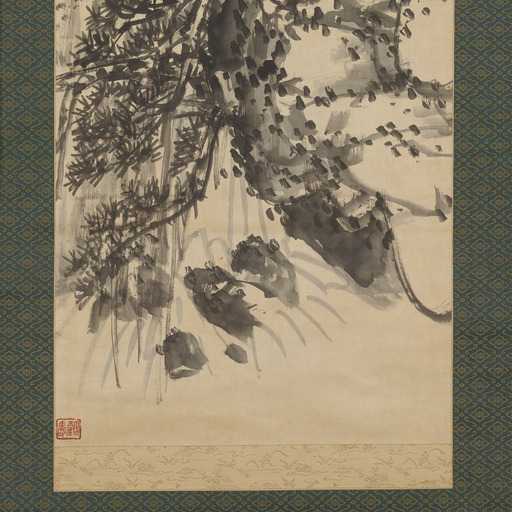
\includegraphics[width=0.2\textwidth, frame]{figures/diffusion/dataset_complete/Painting (1).jpg}}
    \subfigure{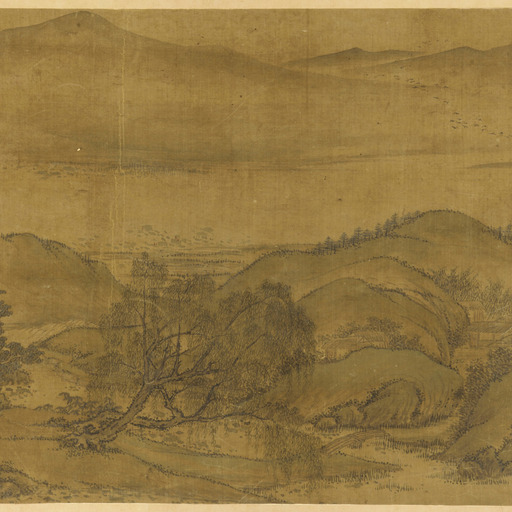
\includegraphics[width=0.2\textwidth, frame]{figures/diffusion/dataset_complete/Painting (2).jpg}}
    \subfigure{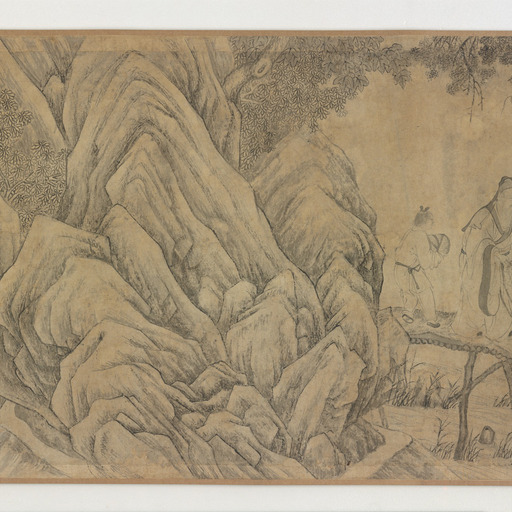
\includegraphics[width=0.2\textwidth, frame]{figures/diffusion/dataset_complete/Painting (3).jpg}}
    \subfigure{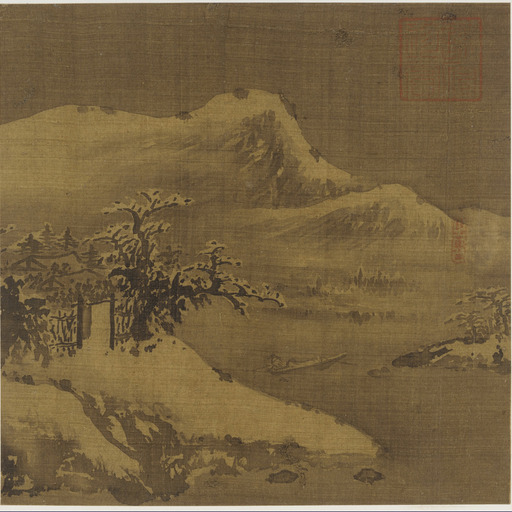
\includegraphics[width=0.2\textwidth, frame]{figures/diffusion/dataset_complete/Painting (4).jpg}}
    \quad
    \subfigure{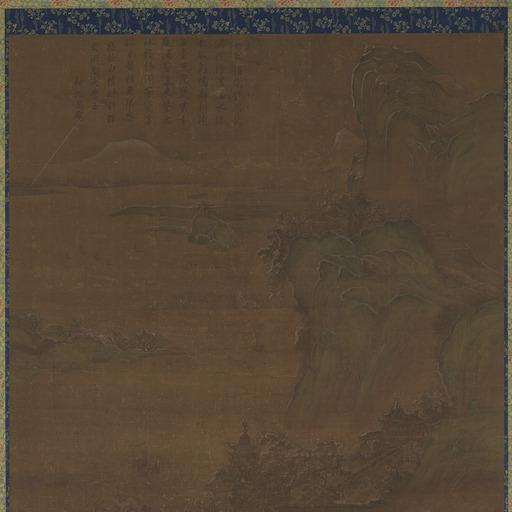
\includegraphics[width=0.2\textwidth, frame]{figures/diffusion/dataset_complete/Painting (5).jpg}}
    \subfigure{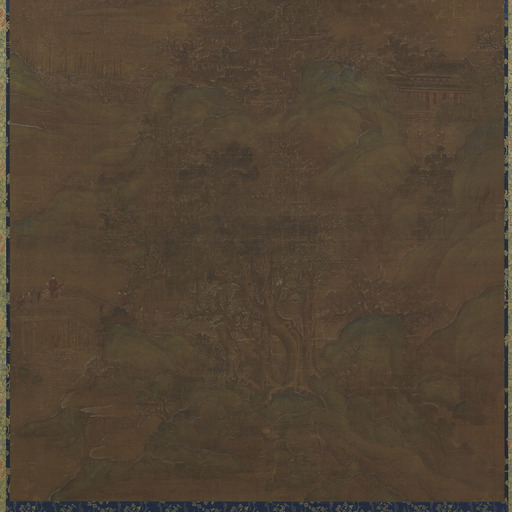
\includegraphics[width=0.2\textwidth, frame]{figures/diffusion/dataset_complete/Painting (6).jpg}}
    \subfigure{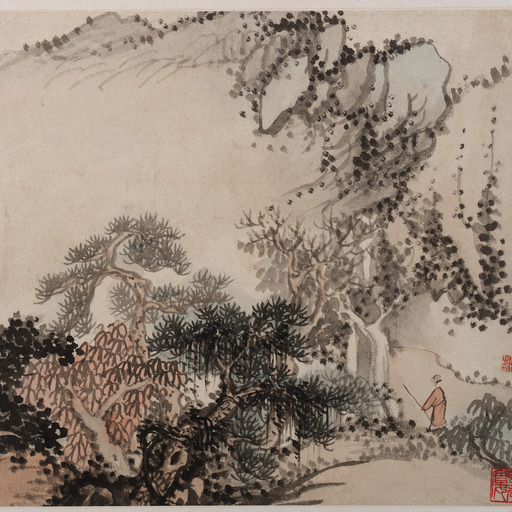
\includegraphics[width=0.2\textwidth, frame]{figures/diffusion/dataset_complete/Painting (7).jpg}}
    \subfigure{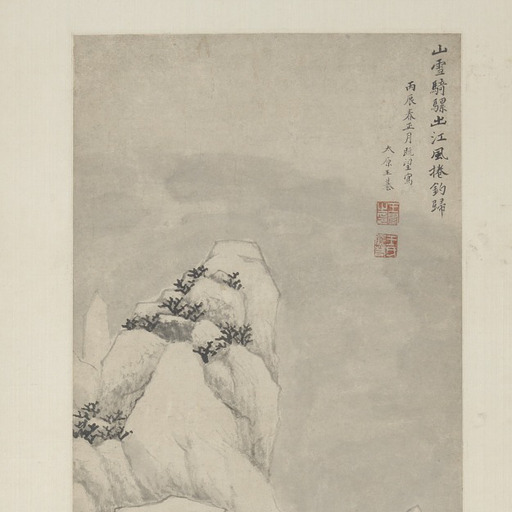
\includegraphics[width=0.2\textwidth, frame]{figures/diffusion/dataset_complete/Painting (8).jpg}}
    \caption{完整数据集中国画样本}\label{fig:complete_dataset_samples}
\end{figure}
\begin{figure}[ht]
    \centering
    \subfigure{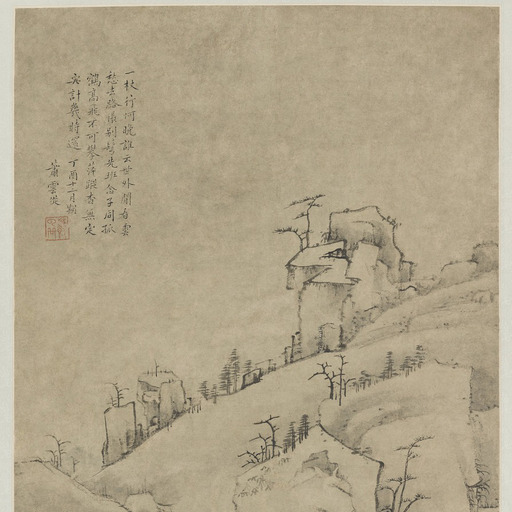
\includegraphics[width=0.2\textwidth, frame]{figures/diffusion/dataset_white/Painting (1).jpg}}
    \subfigure{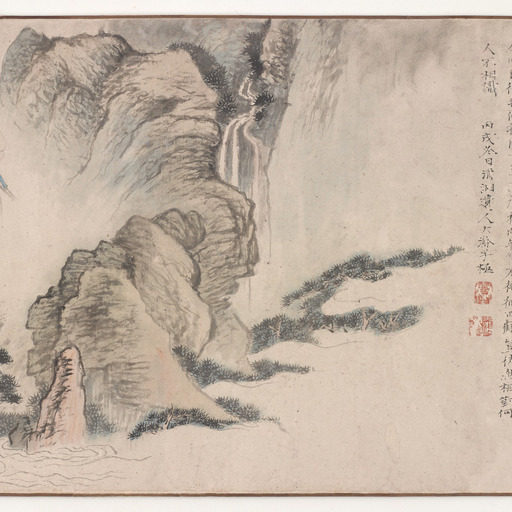
\includegraphics[width=0.2\textwidth, frame]{figures/diffusion/dataset_white/Painting (2).jpg}}
    \subfigure{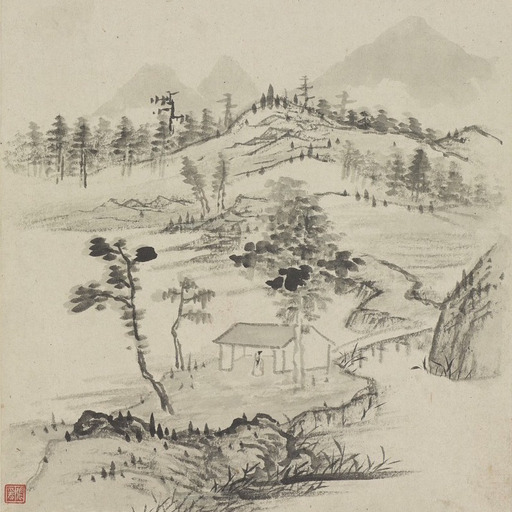
\includegraphics[width=0.2\textwidth, frame]{figures/diffusion/dataset_white/Painting (3).jpg}}
    \subfigure{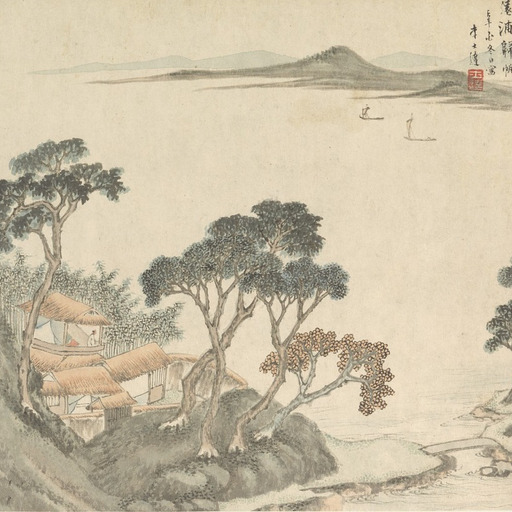
\includegraphics[width=0.2\textwidth, frame]{figures/diffusion/dataset_white/Painting (4).jpg}}
    \quad
    \subfigure{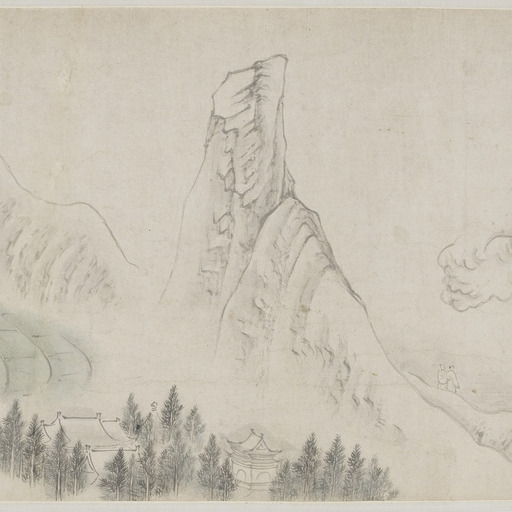
\includegraphics[width=0.2\textwidth, frame]{figures/diffusion/dataset_white/Painting (5).jpg}}
    \subfigure{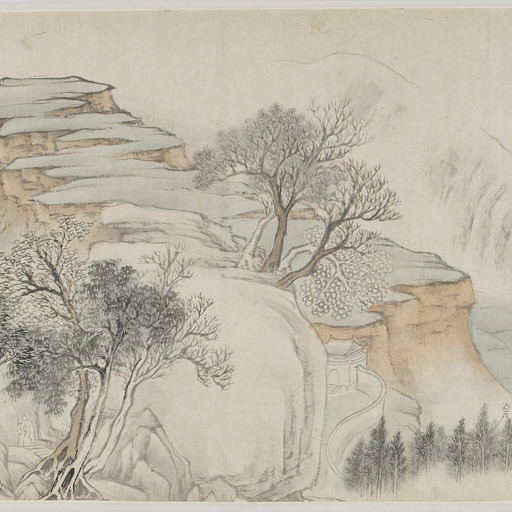
\includegraphics[width=0.2\textwidth, frame]{figures/diffusion/dataset_white/Painting (6).jpg}}
    \subfigure{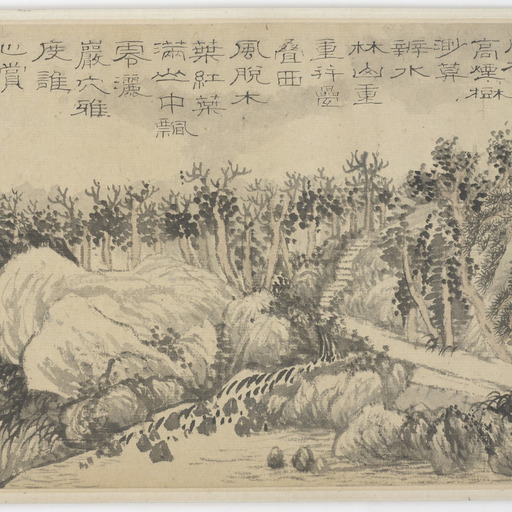
\includegraphics[width=0.2\textwidth, frame]{figures/diffusion/dataset_white/Painting (7).jpg}}
    \subfigure{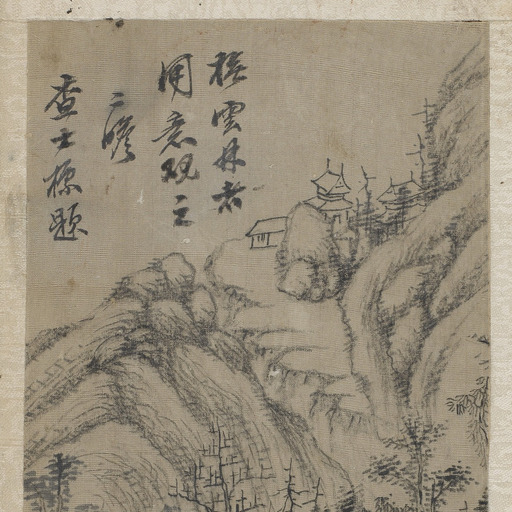
\includegraphics[width=0.2\textwidth, frame]{figures/diffusion/dataset_white/Painting (8).jpg}}
    \caption{浅色中国画数据集样本}\label{fig:white_dataset_samples}
\end{figure}
\begin{figure}[ht]
    \centering
    \subfigure{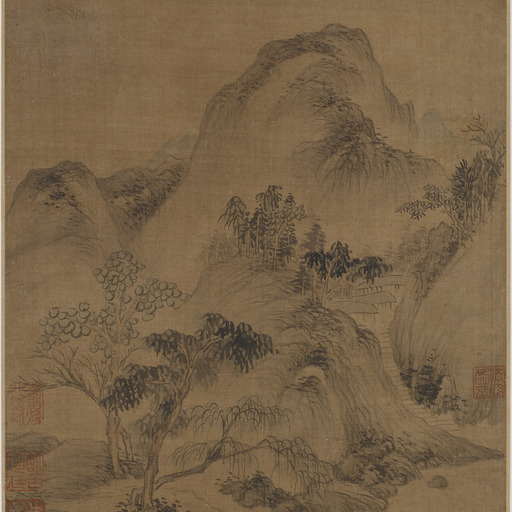
\includegraphics[width=0.2\textwidth, frame]{figures/diffusion/dataset_yellow/Painting (1).jpg}}
    \subfigure{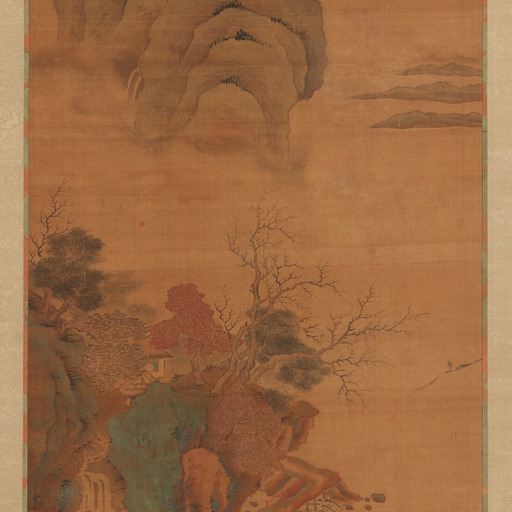
\includegraphics[width=0.2\textwidth, frame]{figures/diffusion/dataset_yellow/Painting (2).jpg}}
    \subfigure{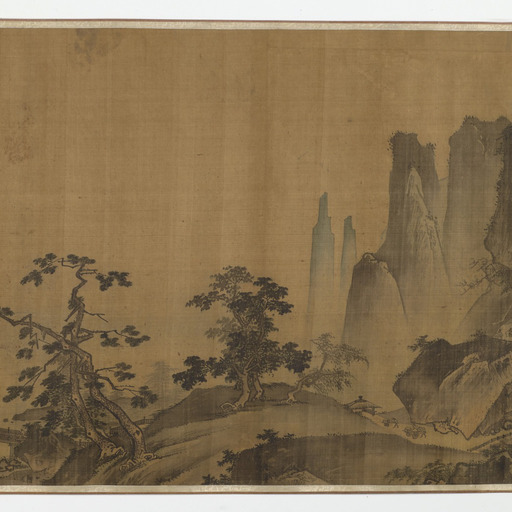
\includegraphics[width=0.2\textwidth, frame]{figures/diffusion/dataset_yellow/Painting (3).jpg}}
    \subfigure{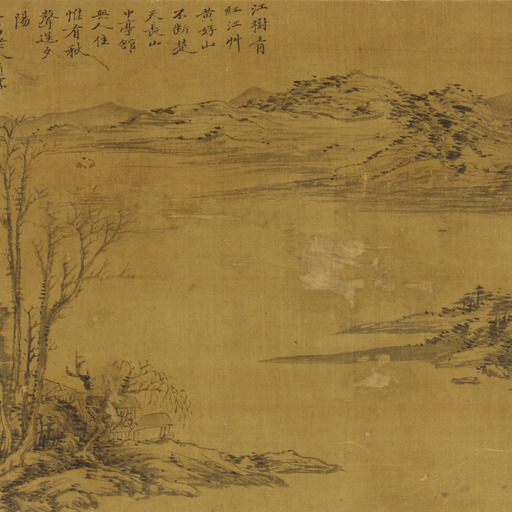
\includegraphics[width=0.2\textwidth, frame]{figures/diffusion/dataset_yellow/Painting (4).jpg}}
    \quad
    \subfigure{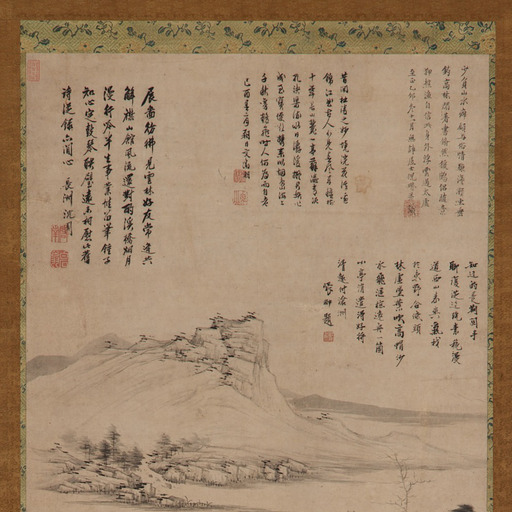
\includegraphics[width=0.2\textwidth, frame]{figures/diffusion/dataset_yellow/Painting (5).jpg}}
    \subfigure{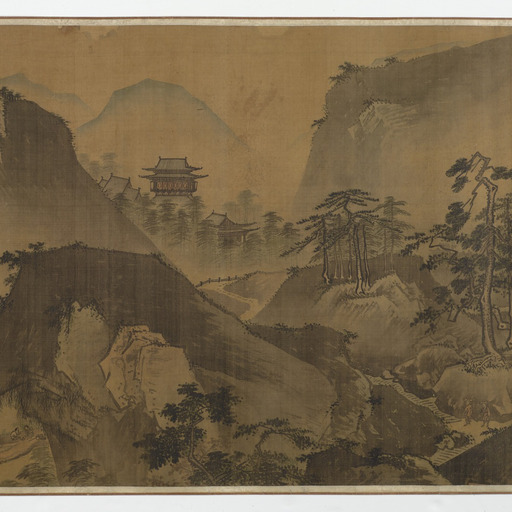
\includegraphics[width=0.2\textwidth, frame]{figures/diffusion/dataset_yellow/Painting (6).jpg}}
    \subfigure{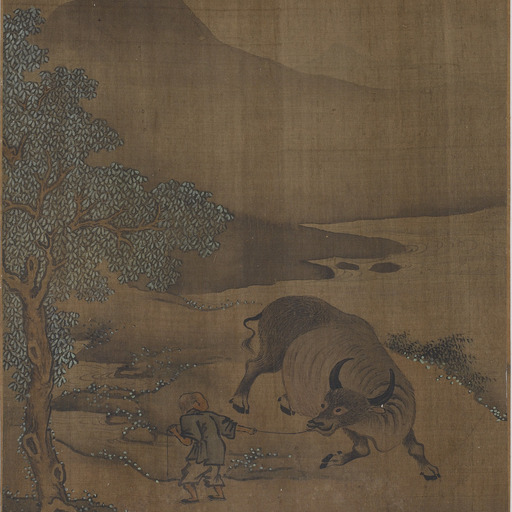
\includegraphics[width=0.2\textwidth, frame]{figures/diffusion/dataset_yellow/Painting (7).jpg}}
    \subfigure{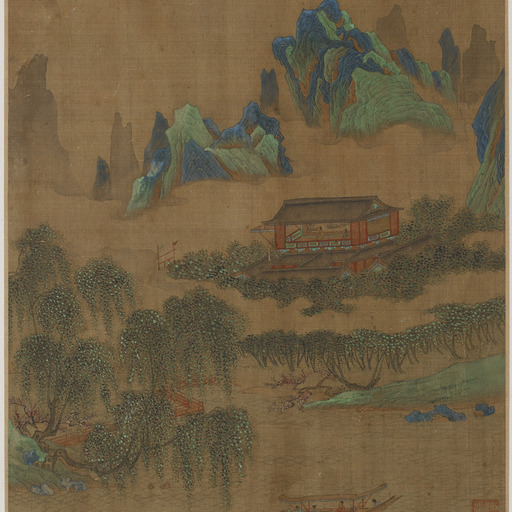
\includegraphics[width=0.2\textwidth, frame]{figures/diffusion/dataset_yellow/Painting (8).jpg}}
    \caption{深色中国画数据集样本}\label{fig:yellow_dataset_samples}
\end{figure}


\section{实验}

分别使用完整数据集、浅色中国画数据集、深色中国画数据集进行训练,
以生成高质量中国画,其中使用浅色中国画数据集依次进行了大批量和小批量训练。

各实验根据实际情况不同,使用不同GPU型号,不同实验共同的环境配置如下:
\begin{itemize}
    \item 操作系统:Ubuntu 20.04
    \item Python 编译器器:Python 3.8
    \item Pytorch 框架:1.12
    \item CUDA 版本:11.3
    \item 编辑器:Visual Studio Code 
\end{itemize}

不同实验扩散模型相同参数设置如下:
\begin{itemize}
    \item 图像大小:128*128
    \item 扩散步骤:1000步
    \item 采样步骤:250步
    \item 损失函数类型:L1距离
    \item 学习率:{$1\times10^{-5}$}
    \item 梯度累计步骤:2
\end{itemize}

\clearpage
\subsection{实验1-完整数据集生成中国画}

\begin{figure}[H]
    \centering
    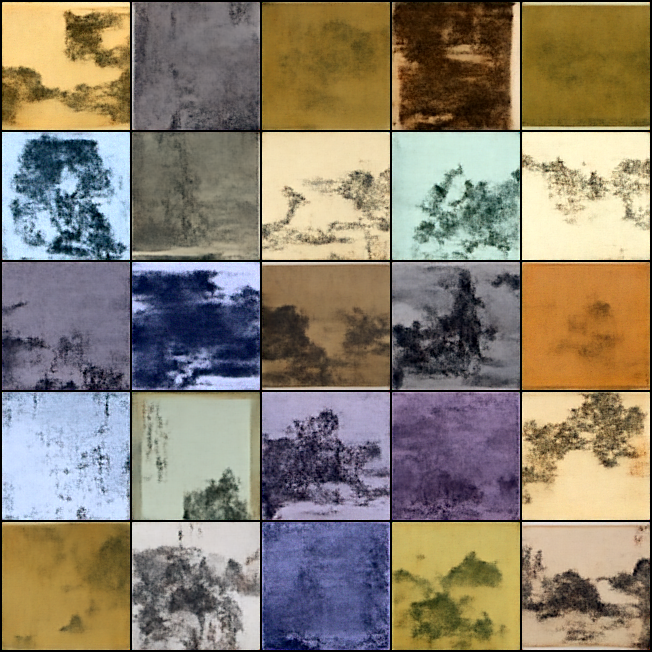
\includegraphics[width=0.8\textwidth]{figures/diffusion/results1/sample-16}
    \caption{实验1-完整数据集生成中国画采样图}\label{fig:diffusion_results1_sample16}
\end{figure}

\subsubsection{实验配置}
使用完整数据集,
在A100- 80GB GPU上,
以128为训练批量训练约15小时。
\subsubsection{实验结果与分析}

实验一结果如图{\ref{fig:diffusion_results1_sample16}}所示。
为减小比对模型不同训练阶段图像生成质量的误差,
采样20次,共获取20张图片并合并显示。
由于完整数据集中图片颜色丰富,
模型需要同时学习不同颜色深度中国画,
在计算资源有限情况下模型收敛需要更长时间,
此外,不同深度中国画混合训练容易造成中国画颜色混合,
降低图片生成质量,
为加快模型收敛与提高图片生成质量,
使用浅色中国画数据集和深色中国画数据集分别训练。

\subsection{实验2-浅色中国画数据集大批量训练}

\begin{figure}[H]
    \centering
    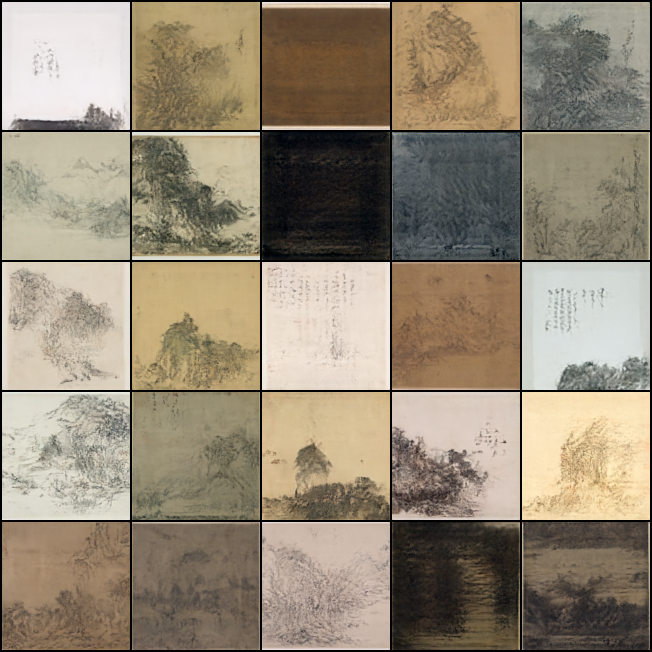
\includegraphics[width=0.8\textwidth]{figures/diffusion/results2/sample-70.png}
    \caption{实验2-浅色中国画数据集大批量训练生成中国画采样图}\label{fig:diffusion_results2_sample70}
\end{figure}

\subsubsection{实验配置}
使用浅色中国画数据集,
在A100- 40GB GPU上,
以64为训练批量,
训练约48小时。
\subsubsection{实验结果与分析}

图{\ref{fig:diffusion_results2_sample70}}为训练70轮后的采样图像,
相比于实验1使用完整数据集所生成的图像,
大部分图像颜色较浅,图像质量明显提升。
第四行{\footnote{以图像表格上方为第一行,左侧为第一列,坐标表示为(行,列)}}图像取得了与中国画非常相似的效果,
一些图像如{$(3,3),(3,5)$},已经可以生成与中国画中的落款相似的文字符号。
同时有一些图像如{$(2,3),(5,4)$},未成功生成中国画,
增大数据集容量、或使用数据增强技术,有望改善扩散模型无法将隐变量噪声空间映射到中国画空间的情况。






\subsection{实验3-浅色中国画数据集小批量训练}

\begin{figure}[H]
    \centering
    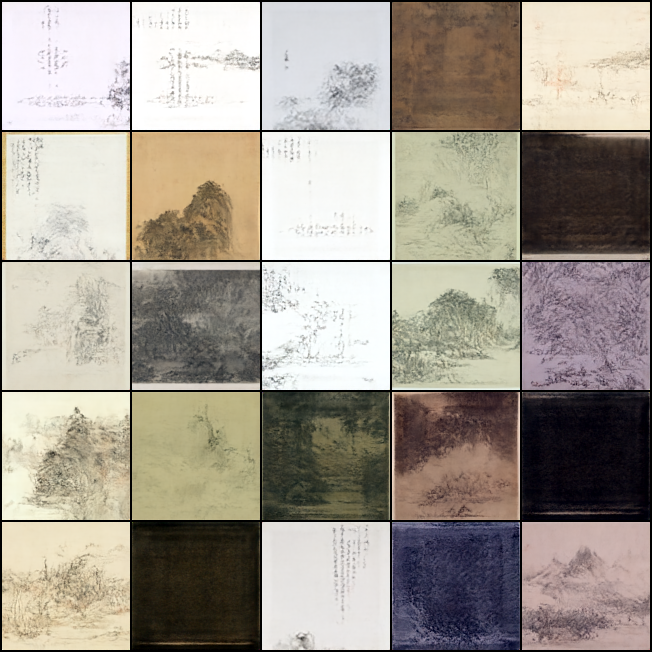
\includegraphics[width=0.8\textwidth]{figures/diffusion/results3/sample-80.png}
    \caption{实验3-浅色中国画数据集小批量训练生成中国画采样图}\label{fig:diffusion_results3_sample80}
\end{figure}

\subsubsection{实验配置}
使用浅色中国画数据集,
在3090- 24GB GPU上,
以32为训练批量训练约48小时。
\subsubsection{实验结果与分析}
图{\ref{fig:diffusion_results3_sample80}}为训练80轮后的采样图像,
相比于实验2,实验三仅仅改变了训练批量,
但产生了更多的无法成功生成中国画的情况,
如子图{$(2,5),(4,2),(4,5),(5,2),(5,4)$}生成颜色过深图像,
子图{$(1,1),(1,2),(1,5),(2,3),(3,3)$}生成颜色过浅图像。
对比实验2与实验3可得,更大的训练批量有助于生成更高质量的中国画。





\subsection{实验4-深色中国画数据集生成中国画}

\begin{figure}[H]
    \centering
    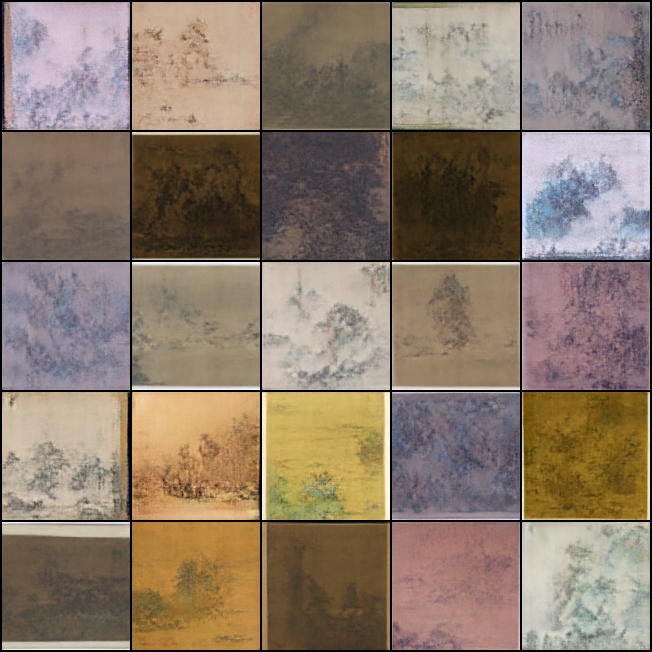
\includegraphics[width=0.8\textwidth]{figures/diffusion/results4/sample-33}
    \caption{实验4-深色中国画数据集生成中国画采样图}\label{fig:diffusion_results4_sample33}
\end{figure}

\subsubsection{实验配置}
使用深色中国画数据集,
在A100- 40GB GPU上,
以64为训练批量训练约36小时。
\subsubsection{实验结果与分析}


图{\ref{fig:diffusion_results4_sample33}}为训练33轮后的采样图像。
实验4与实验2类似,训练批量都为64,都在A100- 40GB GPU上训练。
不同的是,实验4使用深色中国画数据集,而实验2使用浅色中国画数据集。
实验4相对于实验1,得到的图像与中国画更相似;
相比于实验2,生成的中国画的颜色更加丰富。




\ctexset{
    chapter={
        name={},
        number = \arabic{chapter},
        format={\centering\bfseries\heiti\zihao{-3}},
        aftername={\quad}, 
        beforeskip={.5\baselineskip},
        afterskip={.5\baselineskip},
    }
}
\chapter*{结论}
本文对各种主流生成模型进行了探索,
对生成模型进行了分类,
随后将扩散模型应用在中国画生成领域。

可以根据是否直接定义概率密度函数,
将生成模型分为显式密度模型和隐式密度模型。
显式密度模型可以直接表示似然函数,其中,
似然函数可以直接求解的模型主要有规范化流模型和自回归模型,
通过近似方法求解似然函数的模型主要有基于能量的模型、变分自编码器和扩散模型。
隐式密度模型不通过似然函数进行训练,
而使用其他方式与数据分布进行交互,
生成对抗网络是隐式密度模型的主要代表。

使用扩散模型生成中国画,在计算资源有限的情况下,
根据中国画不同的风格训练不同的扩散模型,有助于提升中国画生成质量与加快模型收敛速度,提高训练批量也有助于提高生成中国画的质量。
将生成模型应用于中国画生成有助于继承和弘扬中华优秀传统文化。

近年来生成模型发展迅速,
但有关生成模型整体性介绍的资料仍然缺少,
而对生成模型领域的整体性把握,
有助于以系统的思维设计生成模型算法,
有利于对生成模型的研究。
更广泛地说,2006年《模式识别与机器学习》一书成为机器学习领域经典书籍,
2016《深度学习》一书促进了深度学习的知识普及与发展,
生成模型领域仍缺少一本系统性书籍来促进生成模型的研究与应用,
一本关于“生成模型”的书籍是值得期待的。
此外,未来可考虑获取更多中国画或使用数据增强技术,以增大训练集来获得更好的图像生成效果。
此外,还可考虑将生成模型应用于其他传统文化,如唐诗宋词、古典乐曲、皮影戏等,以继承和弘扬中华优秀传统文化。


\addcontentsline{toc}{chapter}{结论}
% \bibliography{bibliography}
% \bibliographystyle{unsrt}
\printbibliography[title=参考文献,heading=bibintoc]
\chapter*{致谢}

首先,感谢指导教师汪鹏老师,
感谢汪鹏老师给予的关于毕业设计的灵活度,
很幸运能在汪鹏老师指导下做出这样一份有意义的毕业设计,
衷心感谢汪鹏老师的指导和教诲。

其次,感谢河北工业大学的教师们,尤其是智能学院的老师们,
感谢老师们授予宝贵知识,
感谢老师们给予的无私帮助。

再要感谢河北工业大学,
回首大学时光,最重要的转折点莫过于转专业至计算机专业,
感谢学校给予的宝贵转专业机会,
让我能够学习更感兴趣的知识。
感谢学校提供的优良学习环境。

最后要感谢我的父母,
感谢父母的付出与支持。
\addcontentsline{toc}{chapter}{致谢}

\appendix
\chapter{基础知识}
\section{数学}

\subsection{线性代数}
\subsubsection{对角矩阵}
除主对角线之外的元素皆为{$0$}的矩阵。

\subsubsection{矩阵乘法}
如果{$A$}是一个{$l\times m$}矩阵,
{$B$}是一个{$m\times n$}矩阵,
则{$AB$}是一个{$l\times n$}矩阵。

\subsubsection{矩阵的迹}
矩阵的迹为矩阵所有对角元素之和,即:
\begin{equation}
    \label{eq:matrix_trac}
    Tr(A)=\sum_{i}A_{i,i}
\end{equation}

\subsubsection{范数}
范数可以表示向量的大小,范数定义为:
\begin{equation}
    \label{eq:norm}
    {\Vert \bm{x} \Vert}_{p} = {\left(  \sum_{i} \mid x_i  \mid^p    \right)}^{\frac{1}{p}}
\end{equation}
式{\ref{eq:norm}}中,{$p \in \mathbb{R}, p\geq 1$}

{$L^1$}范数为:
\begin{equation}
    \label{eq:l1_norm}
    \Vert \bm{x} \Vert_{1} =  \sum_{i} \mid x_i \mid
\end{equation}

最大范数为:
\begin{equation}
    \label{eq:max_norm}
    \Vert \bm{x} \Vert_{\infty} = \max_i \mid x_i \mid
\end{equation}


矩阵的Frobenius范数为:
\begin{equation}
    \label{eq:frobenius_norm}
    \Vert \bm{x} \Vert_{F} =\sqrt{\sum_{i,j}A_{i,j}^{2}}=\sqrt{Tr(AA^{T})}
\end{equation}

\subsubsection{矩阵行列式}
矩阵的行列式是一个关于方形矩阵(方阵)内所有元素的标量函数值。
一个{$n\times n$}的矩阵{$M$}的行列式为:
\begin{equation}
    \label{eq:determinant_of_matrix}
    \det M =\det
    \begin{bmatrix}
        a_{11}&a_{12}&\cdots &a_{1n} \\
        a_{21}&a_{22}&\cdots &a_{2n} \\
        \vdots & \vdots & & \vdots \\
        a_{n1}&a_{n2}&\cdots &a_{nn}
    \end{bmatrix}
    =\sum_{j_1j_2\cdots j_n}{(-1)}^{\tau (j_1j_2\cdots j_n)}a_{1j_1}a_{2j_2}\ldots a_{nj_n}
\end{equation}

式{\ref{eq:determinant_of_matrix}}中,
求和符号{$\sum $}的下标{$j_1j_2\cdots j_n$}表示集合{$1,2,\ldots ,n$}的全排列,
即共有{$n\!$} 项;
{$\tau({j_1j_2\cdots j_n})$}表示排列{$j_1j_2\cdots j_n$}的符号,
排列的符号定义为式{\ref{eq:parity_of_a_permutation}}。

方阵的行列式可以用来判断矩阵{$M$}是否可逆:
如果{$\det M = 0$},那么矩阵不可逆。

矩阵乘积的行列式等于矩阵行列式的乘积,即:
\begin{equation}
    \det (AB)=\det(A)\det(B)
\end{equation}

\subsubsection{可逆矩阵}
如果一个{$n \times n$}的矩阵{$A$}可逆,那么存在{$n \times n$}矩阵{$B$}使得:
\begin{equation}
    \label{eq:invertable_matrix_defination}
    AB=BA=I_n
\end{equation}

式{\ref{eq:invertable_matrix_defination}}中,{$I_n$}为单位矩阵,并且使用矩阵乘法。

不可逆的方阵又称为奇异矩阵或退化矩阵。

对于可逆矩阵有:
\begin{equation}
    \det(M)\det(M^{-1})=\det(M\dot M^{-1})
    =\det(I)=1
\end{equation}
因此,
\begin{equation}
    \label{eq:determinant_of_inverse_matrix}
    \det (M^{-1})={(\det(M))}^{-1}
\end{equation}




\subsubsection{雅可比矩阵}

假设某函数{$\bm{f}:\mathbb{R}^{n}\rightarrow\mathbb{R}^{m}$},
从{$\bm{x}\in\mathbb{R}^{n}$}映射到向量{$\bm{f(x)}\in\mathbb{R}^{m}$},
这个函数的一阶偏导矩阵称为雅可比矩阵,是一个{$m\times n$}的矩阵。
其第{$i$}行,第{$j$}列的值为{$\bm{J}_{ij}=\frac{\partial f_i}{\partial x_i} $}
\begin{equation}
    \label{eq:jacabian_matrix}
    \bm{J}=
    \begin{bmatrix}
        \frac{\partial f_1}{\partial x_1}& \cdots & \frac{\partial f_1}{\partial x_n}\\
        \vdots &\ddots  & \vdots \\
        \frac{\partial f_m}{\partial x_1}& \cdots & \frac{\partial f_m}{\partial x_n}
    \end{bmatrix}
\end{equation}









\subsection{概率论}
\subsubsection{概率密度函数}
一个连续随机变量{$X$}的概率可以由概率密度函数表示:
\begin{equation}
    p(X\in A )= \int_A f_{\bm{X}}(x)dx
\end{equation}
\subsubsection{概率质量函数}
一个离散随机变量{$X$}的概率可以由概率质量函数表示:
\begin{equation}
    p_{X}(x)=p(\{X=x\})
\end{equation}
\subsubsection{正态分布}
若实值随机变量{$X$}服从正态分布(高斯分布),
则其概率密度函数为:
\begin{equation}
    \label{eq:gaussian_distribution}
    f(x)=\frac{1}{\sigma\sqrt{2\pi}}\exp({\frac{1}{2}{(\frac{x-\mu}{\sigma})}^{2}})
\end{equation}
记为:{$X\sim \mathcal{N}(\mu,\sigma^{2})$}

两高斯分布之和仍为高斯分布,
假设{$X,Y$}为两独立随机变量,
且
\begin{align}
    X\sim & \mathcal{N}(\mu_X,\sigma_{X}^{2}) \\ 
    Y\sim & \mathcal{N}(\mu_Y,\sigma_{Y}^{2}) \\
\end{align}
则{$X,Y$}之和仍为高斯分布,
即:
\begin{align}
    Z=&X+Y\\
    Z\sim& \mathcal{N}(\mu_X+\mu_Y,\sigma_{X}^{2}+\sigma_{Y}^{2})  \label{eq:sum_of_two_gaussian_distributions}
\end{align}

\subsubsection{期望}
当{$x \sim p(x)$},函数{$f(x)$}的期望为:
\begin{equation}
    \label{eq:expection_discrete}
    \mathbb{E}_{x \sim p} [ f(x)] = \sum_{x} p(x)f(x)
\end{equation}
或
\begin{equation}
    \label{eq:expection_continuous}
    \mathbb{E}_{x \sim p} [ f(x)] = \int p(x)f(x) \,dx
\end{equation}

\subsubsection{协方差}
随机变量{$X,Y$}的协方差为:
\begin{equation}
    \label{eq:covariance}
    cov(X,Y)=\mathbb{E}\left[XY\right]-\mathbb{E}\left[X\right]\mathbb{E}\left[Y\right]
\end{equation}


\subsubsection{极大似然估计}

假设{$\theta$}为未知参数(标量或者矢量),
对于服从联合概率质量函数{$p_{X}(\bm{x};\theta)$}的一组观测向量{$X={X_1,\ldots,X_n}$},
假设我们有{$X$}的具体的观测值{$\bm{x}=(x_1,\ldots,x_n)$}。
那么,其极大似然估计是未知参数{$\theta$}的一个取值,
该取值能够使函数{$p_{X}(x_1,\ldots,x_n;\theta)$}取得最大值。
\begin{equation}
    \label{eq:maximux_likelihood_estimation_orgin}
    \hat{\theta_n}
    =\argmax_{\theta} p_X(\bm{x};\theta)
    =\argmax_{\theta} p_X(x_1,\ldots,x_n;\theta)
\end{equation}



\begin{figure}[ht]
    \centering
    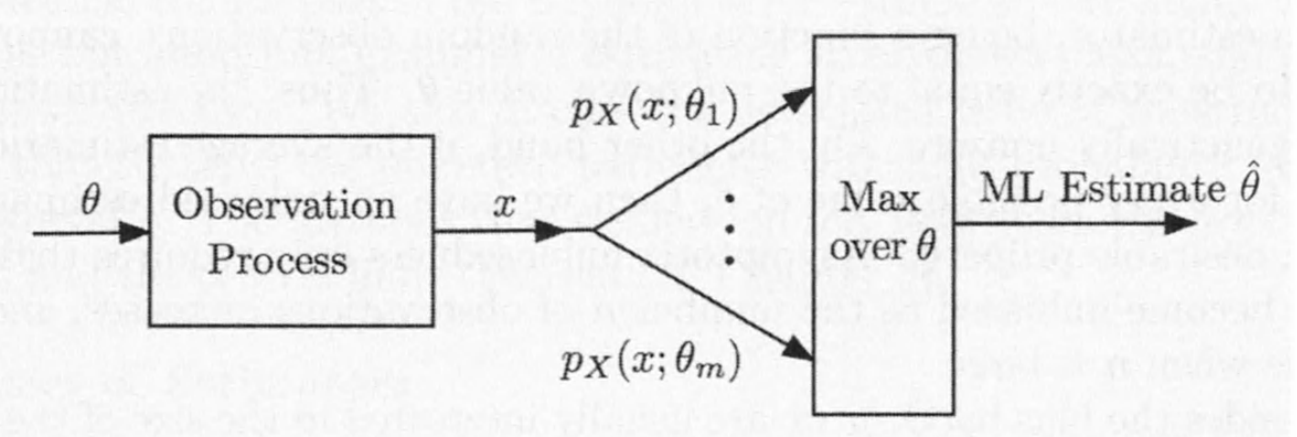
\includegraphics[width=0.8\textwidth]{figures/maximux_likelihood_estimation}
    \caption{极大似然估计示意图}\label{fig:maximux_likelihood_estimation}
\end{figure}

图{\ref{fig:maximux_likelihood_estimation}}中,
假设{$X$}为离散变量,
未知参数{$\theta$}可以从{$\theta_1,\ldots,\theta_m$}中选取。
给定观测值{$X=\bm{x}$},
对于每个{$\theta_i$}取值,
都可以计算{$p_X(\bm{x};\theta_i)$}。
使函数{$p_X(\bm{x};\theta)$}取得最大值的{$\theta_i$}即为极大似然估计{$\theta$}。

在很多情况下,都假定观测向量中的每一个{$X_i$}为互相独立的,
因此,似然函数通常可以改写为:
\begin{equation}
    \label{eq:maximux_likelihood_estimation_discrete}
    p_X(x_1,\ldots,x_n;\theta)=\prod_{i=1}^{n}p_{X_i}(x_i;\theta)
\end{equation}

为了分析与计算方便,可以将其改写为对数似然函数:
\begin{equation}
    \label{eq:maximux_likelihood_estimation_discrete_log}
    \log p_X(x_1,\ldots,x_n;\theta)
    =\log \prod_{i=1}^{n}p_{X_i}(x_i;\theta) 
    =\sum_{i=1}^{n} \log p_{X_i}(x_i;\theta)
\end{equation}

当{$X$}为连续变量时,由概率密度函数替换概率质量函数可得:
\begin{equation}
    \label{eq:maximux_likelihood_estimation_continuous_log}
    \log f_X(x_1,\ldots,x_n;\theta)
    =\log \prod_{i=1}^{n}f_{X_i}(x_i;\theta) 
    =\sum_{i=1}^{n} \log f_{X_i}(x_i;\theta)
\end{equation}

值得注意的是,
对于{$X$}的观测值{$\bm{x}$},
其似然函数{$p_X(\bm{x};\theta)$}并不是指未知 参数取值为{$\theta$}的概率,
而是指在未知参数取值为{$\theta$}时,
{$X$}的观测值为{$\bm{x}$}的概率。

\subsubsection{边缘似然}
边缘似然是似然函数在参数空间上的积分,
表示生成观测样本的概率,
因此,边缘似然也被称为模型证据,简称为证据。




\subsubsection{全概率公式}

全概率公式将对一复杂事件A的概率求解问题转化为了在不同情况下发生的简单事件的概率的求和问题。

若事件{$B_1,B_2,\dots,B_n$}构成一个完备事件组且都有正概率,则有,
\begin{align}
    p(A)
    & =p(AB_1)+p(AB_2)+ \cdots +p(AB_n) \label{eq:total_probability_theorem_1}\\
    & =p(A|B_1)p(B_1)+p(A|B_2)p(B_2)+ \cdots + p(A|B_n)p(B_n) \label{eq:total_probability_theorem_2}
\end{align}




\subsubsection{贝叶斯定理}
若事件{$B_1,B_2,\dots,B_n$}构成一个完备事件组且都有正概率,则有,
\begin{align}
    p(B_i|A)
    & =\frac{p(A|B_i)p(B_i)}{p(A)} \label{eq:bayes_rule_1}\\
    & =\frac{p(A|B_i)p(B_i)}{p(A|B_1)p(B_1)+p(A|B_2)p(B_2)+ \cdots +p(A|B_n)p(B_n)} \label{eq:bayes_rule_2}
\end{align}

在式{\ref{eq:bayes_rule_1}}与{\ref{eq:bayes_rule_2}}中,
{$B_i$}通常表示一个命题,如“硬币正面朝上的次数占投掷次数的50\%”;
{$A$}通常表示事实,如“连续多次投掷硬币的结果”。
{$p(B_i)$}表示{$B_i$}的先验概率,
先验概率为不考虑事实{$A$}时,
人们对事件{$B_i$}的相信程度,
其也包含了人们对于{$B_i$}的先验知识。
{$p(A|B_i)$}为似然函数,
表示当命题{$B_i$}发生时,
事实{$A$}发生的概率。
“似然”表达了事件{$A$}对命题{$B_i$}的支撑程度。
{$p(B_i|A)$}为{$B_i$}的后验概率,
表示考虑事实{$A$}后,
命题{$B_i$}发生的概率。
贝叶斯定理根据事实{$B_i$},
对先验概率{$p(B_i)$}进行更新。

\subsubsection{贝叶斯推理}
贝叶斯推理可以由先验概率和似然函数得出后验概率,
其中先验概率和似然函数皆由统计模型关于观测数据产生。
\begin{equation}
    \label{eq:bayesian_inference}
    p(H\mid E)=\frac{p(E \mid H)p(H)}{p(E)}
\end{equation}
式{\ref{eq:bayesian_inference}}中:
\begin{itemize}
    \item {$H$}为假设,其概率受数据(以下称为证据)影响。
    \item {$p(H)$}为先验概率,是在获得数据{$E$}前,对假设{$H$}概率的估计,{$E$}为当前证据。
    \item {$E$}为证据,即未参与先验概率{$p(H)$}计算的数据。
    \item {$p(H\mid E)$}未后验概率,给出证据{$E$}后,{$H$}为真的概率,是关于{$H$}的函数。
    \item {$p(E\mid H)$}为似然函数,给出假设{$H$}后观测到{$E$}的概率,是关于{$E$}的函数。
    \item {$p(E)$}为边缘似然,也称为模型证据。表示从先验概率中获得观测样本的概率。
\end{itemize}


\subsubsection{蒙特卡洛方法}

蒙特卡洛方法是依赖于随机采样来获得数值结果的一种计算方法。
其底层思想是,用随机方法来解决原理上具备确定性的问题。
在物理和数学上,当其他方法不可用时,常常采用蒙特卡洛方法。
蒙特卡洛方法主要应用于三类问题:优化、数值积分与从概率分布中采样。

当无法精确求和或者计算积分时,
通常使用蒙特卡洛采样方法来近似。
基本思想为,将其和或者积分视为某分布的期望,
通过相应的计算来近似该期望。
如:
\begin{equation}
    \label{eq:monte_carlo_sampling_sum}
    s=\sum_{\bm{x}} p(\bm{x})f(\bm{x})=E_p[f(\bm{x})]
\end{equation}
\begin{equation}
    \label{eq:monte_carlo_sampling_integral}
    s=\int  p(\bm{x})f(\bm{x}) \,d\bm{x}=E_p[f(\bm{x})]
\end{equation}

式{\ref{eq:monte_carlo_sampling_sum}}中,
{$p(\bm{x})$}为随机变量{$\bm{x}$}的概率分布,
式{\ref{eq:monte_carlo_sampling_integral}}中,
{$p(\bm{x})$}为随机变量{$\bm{x}$}的概率密度。

\subsubsection{随机微分方程}
随机微分方程(Stochastic differential equation)是添加了一项或多项随机项的微分方程。



\subsubsection{对比散度}

用函数{$f(x;\bm{\theta})$}来为数据点的概率分布建模,
其中,
{$x$}为模型的输入,
{$\bm{\theta}$}为模型的参数,
且要保证概率积分为1的性质,即:
\begin{equation}
    \label{eq:contrastive_divergence_evidence_p}
    p(x;\bm{\theta})=\frac{f(x;\bm{\theta})}{Z(\bm{\theta})}
\end{equation}
式{\ref{eq:contrastive_divergence_evidence_p}}中,
{$Z(\bm{\theta})$}为划分函数:
\begin{equation}
    \label{eq:contrastive_divergence_evidence_z}
    Z(\bm{\theta})=\int f(x;\bm{\theta}) \,dx
\end{equation}
假定数据点集合为{$\bm{x}=x_1, \ldots, x_K$},
则其似然函数为:
\begin{equation}
    \label{eq:contrastive_divergence_likelihood}
    p(\bm{x};\bm{\theta})=\prod_{k=1}^{K} \frac{f(x_k;\bm{\theta})}{Z(\bm{\theta})}
\end{equation}
极大化似然函数{\ref{eq:contrastive_divergence_likelihood}}等价于最小化负对数似然函数,
即能量函数{$E(\bm{x};\bm{\theta})$}:
\begin{equation}
    \label{eq:contrastive_divergence_energy_function}
    E(\bm{x};\bm{\theta})
    = \log Z(\bm{\theta}) - \frac{1}{K} \sum_{i=1}^{K} \log f(x_i;\bm{\theta})
\end{equation}
对式{\ref{eq:contrastive_divergence_energy_function}}关于参数{$\bm{\theta}$}求偏导,
即:
\begin{align}
    \frac{\partial E(\bm{x};\bm{\theta})}{\partial \bm{\theta}}
    &= \frac{\partial  \log Z(\bm{\theta}) }{\partial \bm{\theta}} -  \frac{1}{K}  \sum_{i=1}^{K} \frac{\partial \log f(x_i;\bm{\theta})}{\partial \bm{\theta}} \\
    &= \frac{\partial  \log Z(\bm{\theta}) }{\partial \bm{\theta}} - \mathbb{E}_{p_{data}}  \left [ \frac{\partial \log f(x;\bm{\theta})}{\partial \bm{\theta}} \right ] \\
    &= \frac{1}{Z(\bm{\theta})} \frac{\partial  Z(\bm{\theta}) }{\partial \bm{\theta}} - \mathbb{E}_{p_{data}}  \left [ \frac{\partial \log f(x;\bm{\theta})}{\partial \bm{\theta}} \right ] \\
    &= \frac{1}{Z(\bm{\theta})}  \frac{\partial  \int f(x;\bm{\theta}) \,dx }{\partial \bm{\theta}}     - \mathbb{E}_{p_{data}}  \left [ \frac{\partial \log f(x;\bm{\theta})}{\partial \bm{\theta}} \right ] \\
    &=  \frac{1}{Z(\bm{\theta})} \int \frac{\partial   f(x;\bm{\theta})  }{\partial \bm{\theta}}   \,dx    - \mathbb{E}_{p_{data}}  \left [ \frac{\partial \log f(x;\bm{\theta})}{\partial \bm{\theta}} \right ] \\
    &=   \frac{1}{Z(\bm{\theta})} \int  f(x;\bm{\theta})  \frac{\partial \log  f(x;\bm{\theta}) }{\partial \bm{\theta}}   \,dx     - \mathbb{E}_{p_{data}}  \left [ \frac{\partial \log f(x;\bm{\theta})}{\partial \bm{\theta}} \right ] \\
    &=  \int  p(x;\bm{\theta})  \frac{\partial \log  f(x;\bm{\theta}) }{\partial \bm{\theta}}   \,dx    - \mathbb{E}_{p_{data}}  \left [ \frac{\partial \log f(x;\bm{\theta})}{\partial \bm{\theta}} \right ] \\
    &=   \mathbb{E}_{p(x;\bm{\theta})} \left [      \frac{\partial \log  f(x;\bm{\theta}) }{\partial \bm{\theta}}      \right ]   - \mathbb{E}_{p_{data}}  \left [ \frac{\partial \log f(x;\bm{\theta})}{\partial \bm{\theta}} \right ] \label{eq:contrastive_divergence_partial_negative_log_likelihood}
\end{align}
式{\ref{eq:contrastive_divergence_partial_negative_log_likelihood}}即为对比散度的梯度,
对于其等号右侧第一项
\begin{equation}
    \mathbb{E}_{p(x;\bm{\theta})} \left [      \frac{\partial \log  f(x;\bm{\theta}) }{\partial \bm{\theta}}      \right ]
\end{equation}
可以通过多次循环使用马尔科夫链蒙特卡洛采样来将训练集数据转化为从{$p(x;\bm{\theta})$}分布中的采样。
假设{$\bm{x}^{n}$}表示对训练样本数据{$\bm{x}$}使用{$n$}次马尔科夫链蒙特卡洛采样获得数据,
可令{$\bm{x}^{0}=\bm{x}$},
即得:
\begin{equation}
    \label{eq:contrastive_divergence_gradient_mcmc_infinite}
    \frac{\partial E(\bm{x};\bm{\theta})}{\partial \bm{\theta}}
    =   \mathbb{E}_{\bm{x}^{\infty}} \left [      \frac{\partial \log  f(x;\bm{\theta}) }{\partial \bm{\theta}}      \right ]   - \mathbb{E}_{\bm{x}^{0}}  \left [ \frac{\partial \log f(x;\bm{\theta})}{\partial \bm{\theta}} \right ]
\end{equation}
对于式{\ref{eq:contrastive_divergence_gradient_mcmc_infinite}},在机器学习中,
即使使用一次马尔科夫链蒙特卡洛采样也可以取得很好得效果,
参数更新式为:
\begin{equation}
    \bm{\theta}_{t+1}=\bm{\theta}_{t} + \eta \left(  \mathbb{E}_{\bm{x}^{0}} \left [      \frac{\partial \log  f(x;\bm{\theta}) }{\partial \bm{\theta}}      \right ]   - \mathbb{E}_{\bm{x}^{1}}  \left [ \frac{\partial \log f(x;\bm{\theta})}{\partial \bm{\theta}} \right ] \right) 
\end{equation}


\subsubsection{证据下界}
显式密度模型需要表示出概率密度函数,
假定观测变量{$\bm{x}$}和隐变量{$\bm{z}$}构成联合概率分布{$p(\bm{x},\bm{z})$},
概率密度函数{$p(\bm{x})$}可表示为:
\begin{equation}
    \label{eq:elbo_probability_of_x_with_integral}
    p(\bm{x})=\int p(\bm{x},\bm{z})\,d\bm{z}
\end{equation}
或使用概率链式法则:
\begin{equation}
    \label{eq:elbo_probability_of_x_chain_rule}
    p(\bm{x})=\frac{p(\bm{x},\bm{z})}{p(\bm{z}\mid\bm{x})}
\end{equation}
对于式{\ref{eq:elbo_probability_of_x_with_integral}},
复杂模型无法对所有隐变量{$\bm{z}$}进行积分;
对于式{\ref{eq:elbo_probability_of_x_chain_rule}},
因无法获得实际后验分布{$p(\bm{z}\mid\bm{x})$}
而也无法直接计算。
结合式{\ref{eq:elbo_probability_of_x_with_integral}}与式{\ref{eq:elbo_probability_of_x_chain_rule}},有:
\begin{align}
    \log p(\bm{x})
    & =\log \int p(\bm{x},\bm{z}) d\,z & \mbox{(根据式{\ref{eq:elbo_probability_of_x_with_integral}})} \\
    &=\log \int p(\bm{x},\bm{z})  \frac{q_{\phi}(\bm{z}\mid\bm{x})}{q_{\phi}(\bm{z}\mid\bm{x})} d\,z \\
    &=\log \int \frac{p(\bm{x},\bm{z}) q_{\phi}(\bm{z}\mid\bm{x})}{q_{\phi}(\bm{z}\mid\bm{x})} d\,z \\
    &=\log \int q_{\phi}(\bm{z}\mid\bm{x}) \frac{p(\bm{x},\bm{z}) }{q_{\phi}(\bm{z}\mid\bm{x})} d\,z \\
    &= \log \mathbb{E}_{q_{\phi}(\bm{z}|\bm{x})}\left[\frac{p(\bm{x},\bm{z})}{q_{\phi}(\bm{z}\mid\bm{x})}\right]  & \mbox{(根据期望定义式{\ref{eq:expection_continuous}})} \\
    &\geq \mathbb{E}_{q_{\phi}(\bm{z}|\bm{x})}\left[\log\frac{p(\bm{x},\bm{z})}{q_{\phi}(\bm{z}\mid\bm{x})}\right] & \mbox{(根据杰森不等式{\ref{eq:Jensen_ineuqality}})} \label{eq:elbo_jensen_inequaality}
\end{align}
可获得观测变量{$\bm{x}$}对数似然函数的证据下界(Evidence Lower BOund, ELBO):
\begin{equation}
    \label{eq:evidence_lower_bound}
     \mathbb{E}_{q_{\phi}(\bm{z}|\bm{x})}\left[\log\frac{p(\bm{x},\bm{z})}{q_{\phi}(\bm{z}\mid\bm{x})}\right]
\end{equation}
其中,{$q_{\phi}(\bm{z}|\bm{x})$}是由参数{$\phi$}确定的近似变分分布,最大化证据下界即优化参数{$\phi$}。
最大化证据下界可以取得与极大似然估计相近的效果。

此外,对证据下界的另一种证明方式能够体现最大化证据下界的原因,
\begin{align}
    \log p(\bm{x})
    &=\log p(\bm{x}) \int q_{\phi}(\bm{z}\mid\bm{x})d\,\bm{z}     & \mbox{({$1=\int q_{\phi}(\bm{z}\mid\bm{x})d\,\bm{z} $})}\\
    &=\int q_{\phi}(\bm{z}\mid\bm{x})(\log p(\bm{x})) d\,\bm{z}     & \mbox{(不改变积分值)}\\
    &=\mathbb{E}_{q_{\phi}(\bm{z}|\bm{x})} \left[  \log p(\bm{x}) \right] & \mbox{(期望定义式{\ref{eq:expection_continuous}})}\\
    &=\mathbb{E}_{q_{\phi}(\bm{z}|\bm{x})} \left[  \log \frac{p(\bm{x},\bm{z})}{p(\bm{z}\mid \bm{x})}  \right] & \mbox{(根据式{\ref{eq:elbo_probability_of_x_chain_rule}})}\\
    &=\mathbb{E}_{q_{\phi}(\bm{z}|\bm{x})} \left[  \log \frac{p(\bm{x},\bm{z})q_{\phi}(\bm{z}|\bm{x})}{p(\bm{z}\mid \bm{x})q_{\phi}(\bm{z}|\bm{x})}  \right] & \mbox{({$1=\frac{q_{\phi}(\bm{z}\mid\bm{x})}{q_{\phi}(\bm{z}\mid\bm{x})}$})}\\
    &=\mathbb{E}_{q_{\phi}(\bm{z}|\bm{x})} \left[  \log \frac{p(\bm{x},\bm{z})}{q_{\phi}(\bm{z}|\bm{x})}  \right] 
     +\mathbb{E}_{q_{\phi}(\bm{z}|\bm{x})} \left[  \log \frac{q_{\phi}(\bm{z}|\bm{x})}{p(\bm{z}\mid \bm{x})}  \right] & \mbox{(期望拆分)}\\
    &=\mathbb{E}_{q_{\phi}(\bm{z}|\bm{x})} \left[  \log \frac{p(\bm{x},\bm{z})}{q_{\phi}(\bm{z}|\bm{x})}  \right] + D_{KL}(q_{\phi}(\bm{z}|\bm{x}) \mid \mid p(\bm{z}\mid \bm{x})) & \mbox{(散度定义式{\ref{eq:kl_divergence}})} \label{eq:elbo_eexpection_and_kl_divergence}\\
    &\geq\mathbb{E}_{q_{\phi}(\bm{z}|\bm{x})} \left[  \log \frac{p(\bm{x},\bm{z})}{q_{\phi}(\bm{z}|\bm{x})}  \right] & \mbox{(根据式{\ref{eq:kl_divergence_geq_zero}})}
\end{align}

根据式{\ref{eq:elbo_eexpection_and_kl_divergence}},
对数似然函数{$\log p(\bm{x})$}即为证据下界与近似后验{$q_{\phi}(\bm{z}|\bm{x})$}和真实后验{$p(\bm{z}\mid \bm{x})$}的KL散度,
KL散度项即为式{\ref{eq:elbo_jensen_inequaality}}中被移除的项。
由于对数似然函数{$\log p(\bm{x})$}与证据下界的差值仅为非负的KL散度项,
因此,证据下界的值不可能超过对数似然函数{$\log p(\bm{x})$}的值。
通过最小化KL散度项,
即可使变分后验{$q_{\phi}(\bm{z}|\bm{x})$}更接近于真实后验{$p(\bm{z}\mid \bm{x})$},
但由于无法获得真实后验{$p(\bm{z}\mid \bm{x})$},
无法直接对KL散度项最小化。
而注意到,
式{\ref{eq:elbo_eexpection_and_kl_divergence}}左侧证据下界项中,
{$p(\bm{x},\bm{z})$}与参数{$\phi$}无关,
对其关于变量{$\bm{z}$}计算边缘概率所得{$p(\bm{x})$}也因此与参数{$\phi$}无关,
即{$\log p(\bm{x})$}与参数{$\phi$}无关。
因此,在改变参数{$\phi$}时,证据下界与KL散度项的和为定值,
对证据下界项的最大化即代表了KL散度项的最小化。
对证据下界项的优化程度可以体现模型对隐变量后验概率的拟合程度,
证据下界项优化程度越高,近似后验则越接近真实后验。
此外,
由于证据下界是对模型证据{$\log p(\bm{x})$}的近似,
模型经过训练后,
证据下界也可以作为对观测数据或生成数据似然的估计。


\subsubsection{重参数方法}
从均值为{$\mu$},
方差为{$\sigma$}的正态分布{$x \sim \mathcal{N} (x;\mu,\sigma^{2})$}中采样过程可以改写为
\begin{equation}
    \label{eq:reparameterization_trick}
    x=\mu+\sigma\epsilon \mbox{\qquad 其中} \sigma\sim\mathcal{N}(\epsilon;0,1)
\end{equation}

使用重参数方法,从任意高斯分布取样可以变为从标准高斯分布取样,
即将标准高斯分布采样取值根据{$\sigma$}对进行伸缩变换,
再根据{$\mu$}进行平移变换。

\subsection{信息论}
\subsubsection{信息论基础}
对信息论最直觉的理解是,某一事件发生携带的信息量,与其发生的概率成反相关。
也就是说,低概率事件的发生,要比更高概率事件的发生携带更多的信息。
如“今天早上有日食”相比“今天早上太阳照常升起”携带更多的信息。
因此,对事件携带信息的量化也需要满足这种直觉。即:
\begin{itemize}
    \item 更高概率发生的事件携带更少的信息,必定发生的事件不携带信息。
    \item 更低概率发生的事件携带更多的信息。
    \item 相互独立的事件携带的信息具有可加性。
\end{itemize}
由此,可以定义事件{$x$}携带的信息为:
\begin{equation}
    \label{eq:information_theory}
    I(x)=-\log p(x)
\end{equation}

式{\ref{eq:information_theory}}中,
{$\log$}表示以自然数{$e$}为底数的自然对数。

\subsubsection{香农熵}
香农熵可以量化事件概率分布中所含的不确定度:
\begin{equation}
    \label{eq:shannon_entropy}
    H(x)=\mathbb{E}_{x \thicksim p}[I(x)]=-\mathbb{E}_{x \thicksim p} [\log p(x)]
\end{equation}


\subsubsection{Kullback-Leibler(KL)散度}
对于一随机变量{$x$}的两个概率分布{$p(x)$}和{$q(x)$},
KL散度可以测量这两个概率分布的不同程度。

\begin{align}
    D_{KL}(p \mid\mid q)
    &=\mathbb{E}_{x \thicksim p} [ \log \frac{p(x)}{q(x)} ] \label{eq:kl_divergence_orgin}\\
    &=\mathbb{E}_{x \thicksim p} [ \log p(x) -  \log q(x)] \label{eq:kl_divergence}
\end{align}

对式{\ref{eq:kl_divergence_orgin}}进行变形:
\begin{align}
    -D_{KL}(p \mid\mid q)
    &=-(\mathbb{E}_{x \thicksim p}[ \log \frac{p(x)}{q(x)} ] )\\
    &=\sum_{x} p(x) \log \frac{q(x)}{p(x)} \\
    &\leq \sum_{x} p(x) ( \frac{q(x)}{p(x)}  - 1 ) \\
    &= \sum_{x} q(x) - \sum_{x}p(x)\\
    &= 1-1\\
    &= 0 \label{eq:kl_divergence_geq_zero}
\end{align}
因此,KL散度具有非负性。 

对于两高斯分布,其KL散度为:
\begin{align}
    &D_{KL}(\mathcal{N}(\bm{x};\bm{\mu}_{x},\bm{\Sigma}_{x})\Vert \mathcal{N}(\bm{y};\bm{\mu}_{y},\bm{\Sigma}_{y}))
   \nonumber \\=& \frac{1}{2}\left[
        \log \frac{\left|  \bm{\Sigma}_{y} \right|}{\left|  \bm{\Sigma}_{x} \right|}
        -d
        +tr(\bm{\Sigma}_{y}^{-1}\bm{\Sigma}_{x})
        +{(\bm{\mu}_{y}-\bm{\mu}_{x})}^{\intercal}\bm{\Sigma}_{y}^{-1}(\bm{\mu}_{y}-\bm{\mu}_{x})
    \right] \label{eq:kl_divergence_of_two_gaussian}
\end{align}

\subsubsection{交叉熵}
交叉熵与KL散度相近,相比于KL散度,交叉熵增加了概率分布{$p(x)$}的香农熵{$H(p)$}:
\begin{align}
    H(p,q)
    &=H(p)+D_{KL}(p \mid \mid q) \\
    &=- \mathbb{E}_{x \sim p}\log q(x) \label{eq:cross_euqation}
\end{align}

因为被省略的项{$H(p)$}与{$q(x)$}无关,
所以关于{$q(x)$}最小化交叉熵{$H(p,q)$}等价于最小化KL散度{$D_{KL}(p \mid \mid q)$}。



\subsubsection{信噪比}
信噪比(Signal-to-noise ratio, SNR, S/N)为有价值信号和背景噪声的比值。
\begin{equation}
    \label{eq:signal_to_noise_ratio}
    SNR=\frac{\mu^{2}}{\sigma^{2}}
\end{equation}
式{\ref{eq:signal_to_noise_ratio}}中,
{$\mu$}为均值,
{$\sigma$}为方差。



\subsection{其他}
\subsubsection{配方法}
若有抛物线{$y=ax^{2}+bx+c(a \neq 0)$},
则可使用配方法求其顶点与对称轴,
\begin{align}
    y&=ax^{2}+bx+c\\
     &= a{(x+\frac{b}{2a})}^{2} + \frac{4ac-b^2}{4a} \label{eq:completing_the_square_method}
\end{align}

由式{\ref{eq:completing_the_square_method}},
抛物线{$y=ax^{2}+bx+c(a \neq 0)$}的对称轴为{$x=-\frac{b}{2a}$},
顶点坐标为{$(-\frac{b}{2a},\frac{4ac-b^2}{4a})$}。


\subsubsection{排列}

排列指对一个集合中所有元素的一种排列。
如果集合{$\mathbb{X} $}确定了集合内部元素的顺序,
其每一种排列{$\sigma$}可以看成对原序列内部元素进行多次置换,
置换会增加集合内逆序对(两元素与原确定顺序不同)的个数,
排列{$\sigma$}的符号即为该排列下逆序对的个数。

排列的符号由{$sgn(\sigma)$}表示,可以表示为:
\begin{equation}
    \label{eq:parity_of_a_permutation}
    sgn(\sigma)={(-1)}^{N(\sigma)}
\end{equation}

其中{$N(\sigma)$}表示排列{$\sigma$}中逆序对的个数、

\subsubsection{S型函数}
S型函数的曲线为S型,常见的S型函数如逻辑斯蒂函数为:
\begin{equation}
    \label{eq:sigmoid_function}
    sigmoid(x)= \frac{1}{1+\exp(-x)}=\frac{\exp(x)}{\exp(x)+1}
\end{equation}

\subsubsection{换元定理在概率中的应用}

若有随机变量{$z\thicksim \pi(z)$}, 
一一映射函数{$x=f(z)$},
函数{$f$}可逆,即{$z=f^{-1}(x)$}。
根据概率分布的定义有:
\begin{equation}
    \int p(x)  \,dx = \int \pi(z)\,dz =1
\end{equation}
对于单元变量有:
\begin{equation}
    p(x)=\pi(z)\left\rvert\frac{dz}{dx}\right\rvert
    =\pi(f^{-1}(x))\left\rvert\frac{df^{-1}}{dx}\right\rvert
    =\pi(f^{-1}(x))\left\rvert(f^{-1})'(x)\right\rvert
\end{equation}
对于多元变量形式{$\bm{z}\thicksim \pi(\bm{z})$},{$\bm{x}=f(\bm{z})$},{$\bm{z}=f^{-1}(\bm{x})$}有:
\begin{equation}
    \label{eq:mutivariable_change_variable_in_probability}
    p(\bm{x})=\pi(\bm{z})\left\rvert \det \frac{d\bm{z}}{d\bm{x}}\right\rvert
    =\pi(f^{-1}(\bm{x}))\left\vert \det \frac{df^{-1}}{d\bm{x}} \right\rvert
\end{equation}
在式{\ref{eq:mutivariable_change_variable_in_probability}}中,
{$\det  \frac{\partial f^{-1}}{\partial x}$}表示函数{$f^{-1}$}的雅可比矩阵行列式。

\subsubsection{反函数定理应用}
对于{$y=f(x)$}和{$x=f^{-1}(y)$},
\begin{equation}
    \label{eq:inverse_function_theorem_application}
    \frac{df^{-1}(y)}{dy}
    =\frac{dx}{dy}
    ={\left(\frac{dy}{dx}\right)}^{-1}
    ={\left(\frac{df(x)}{dx}\right)}^{-1}
\end{equation}

\subsubsection{微分方程}
微分方程是包含了一项或多项函数以及它们的导数的方程。


\subsubsection{杰森不等式}
\begin{equation}
    \label{eq:Jensen_ineuqality}
    \mathbb{E}[g(x)]\geq g(\mathbb{E}[x])
\end{equation}

\subsubsection{指示函数}
一个集合的子集的指示函数,
将集合中属于该子集的元素映射为1,
其他元素映射为0。
假设集合{$X$}有子集{$Y$},则:
\begin{equation}
    1_{A}(x) \coloneqq  
    \begin{cases}
        1 &\mbox{,} x\in A \\
        0 &\mbox{,}x\notin A 
    \end{cases}
\end{equation}


\subsubsection{狄拉克{$\delta$}函数}
狄拉克{$\delta$}函数,也被称为单位脉冲,
是在实数域上除0以外点的值处处为0,
且在整个实数域上积分为1的广义函数或分布。

\subsubsection{狄拉克测量}
狄拉克测量将集合的大小指定为含有特定元素{$x$}的数量。
假设集合{$X$}具有可观测子集{$A$},且{$x \in X$},
则有:
\begin{equation}
    \label{eq:dirac_measure}
    \delta_{(x)}(A)=1_{A}(x)=\begin{cases}
        0 &\mbox{,}x\notin A \\
        1 &\mbox{,}x\in A 
    \end{cases}
\end{equation}
式{\ref{eq:dirac_measure}}中,
{$1_{A}$}为指示函数。

\subsubsection{点评估}
点评估是狄拉克测量积分的描述,
假设{$x \in X$},
则关于点{$y$}的点评估为:
\begin{equation}
    \label{eq:point_evaluation}
    \int_{X}f(x) d\,u =f(y)
\end{equation}

\subsubsection{泛函}
泛函是指以函数构成的向量空间为定义域,
实数为值域的“函数”,
往往被称为“函数的函数”。
在泛函分析中,
泛函也用来指一个从任意向量空间到标量域的映射。


\subsubsection{向量空间}
向量空间是一个内部元素具备可加性和可乘性的集合。

\subsubsection{内积空间}
内积空间是具有内积操作的向量空间。

\subsubsection{欧几里得向量空间}
欧几里得向量空间是在实数域上的有限维度内积空间。

\subsubsection{希尔伯特空间}
希尔伯特空间将欧几里得向量空间扩展至无限维度。

\subsubsection{再生核希尔伯特空间}
在泛函分析中,再生核希尔伯特空间是函数的希尔伯特空间,
其函数的点评估为线性连续泛函。
当两个函数{$f,g$}在再生核希尔伯特空间中在范数上相近,
即{$\Vert f-g \Vert$}值趋近于0,
则对于所有{$x$},{$\Vert f(x)-g(x) \Vert$}趋近于0,
反之不一定成立。

\subsubsection{最大均值差异}
最大均值差异以特征的嵌入均值(Mean Embeddings)来表示距离,
假设{$p,q$}为集合{$\mathcal{X}$}上的概率分布,
特征映射{$\phi: \mathcal{X} \rightarrow \mathcal{H} $},
其中{$\mathcal{H}$}为再生核希尔伯特空间,
则有:
\begin{equation}
    \label{eq:maximux_mean_distance}
    MMD(P,Q)= {\Vert \mathbb{E}_{X \sim P}[\phi(X)] -  \mathbb{E}_{Y \sim Q}[\phi(Y)] \Vert}_{\mathcal{H}}
\end{equation}

\section{物理学}
\subsection{玻尔兹曼分布}
在统计力学与数学中,
玻尔兹曼分布(也成为吉布斯分布)给出了一个系统处在特定状态的概率,
其值与该状态的能量和该系统的热力学温度相关:
\begin{equation}
    \label{eq:boltzmann_equation_without_q}
    p_i \varpropto  \exp(-\frac{\varepsilon_i}{kT})
\end{equation}
式{\ref{eq:boltzmann_equation}}中,
{$p_i$}表示系统处在状态{$i$}的概率,
{$\varepsilon _i$}式该状态的能量,
{$k$}为玻尔兹曼常数,
{$T$}为热力学温度。
{$\varpropto$}表示其成正比。
其比例系数为{$\frac{1}{Q}$},其中
\begin{equation}
    \label{eq:boltzmann_equation_q}
    Q=\sum_{i=1}^{M} \exp(-\frac{\varepsilon_i}{kT})
\end{equation}
结合式{\ref{eq:boltzmann_equation_without_q}}与式{\ref{eq:boltzmann_equation_q}}的
\begin{equation}
    \label{eq:boltzmann_equation}
    p_i = \frac{1}{Q} \exp(-\frac{\varepsilon_i}{kT})
    =\frac{\exp(-\frac{\varepsilon_i}{kT})}{\sum_{i=1}^{M} \exp(-\frac{\varepsilon_i}{kT})}
\end{equation}






\subsection{朗之万动力学}

在物理学中,朗之万动力学是一种对分子系统运动的数学建模方式,是一种采样方式。
朗之万模拟是一种蒙特卡洛模拟。



\section{机器学习与深度学习}
\subsection{概率图模型}

机器学习算法通常涉及到大量随机变量的概率分布。
在通常情况下,这些变量只与很少部分的变量互相影响,
使用单一的函数方程来描述全体变量的联合概率分布不利于进行计算,
而将联合概率分布分解为条件概率有助于减少参数的数量。
如对于三个随机变量{$a,b,c$},
其联合概率分布可以分解为:
\begin{equation}
    p(a,b,c)=p(a)p(b\mid a) p(c \mid a)
\end{equation}

当用“图”来表示这种对联合概率分布的分解时,
即为概率图模型。

概率图模型使用图{$\mathcal{G} $}来对变量进行建模,
图中的每一个节点表示一个随机变量,
每一条边连接两个随机变量,
表示两个变量的概率分布可以直接互相表示。

概率图模型可以分为有向图模型和无向图模型。
\subsubsection{有向图模型}
\begin{figure}[ht]
    \centering
    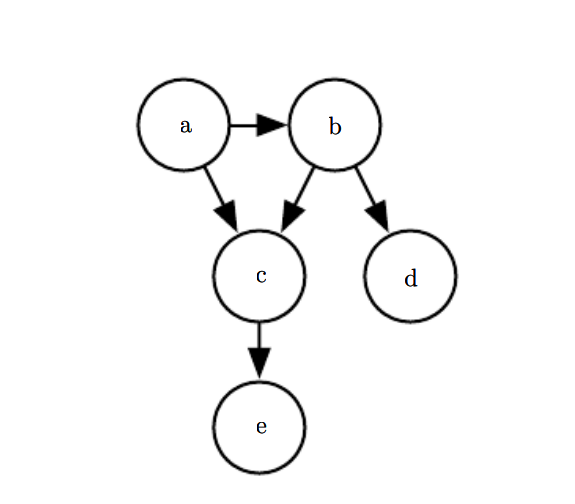
\includegraphics[height=0.3\textheight]{figures/directed_graph_model}
    \caption{有向图模型实例}\label{fig:directed_graph_model}
\end{figure}
有向图模型中的边为有向边。
有向图模型中,
每一个随机变量{$x_i$}都有一个概率因子{$p_{\mathcal{G}}(x_i)$}来表示其条件分布,
即:
\begin{equation}
    \label{eq:directed_graph_model}
    p(\bm{x})=\prod_{i} p(x_i \mid p_{\mathcal{G}}(x_i))
\end{equation}



图{\ref{fig:directed_graph_model}}中,
{$a,b,c,d,e$}为随机变量,
该有向图模型的联合概率分布为:
\begin{align}
    p(a,b,c,d,e)
    &=p(a \mid p_{\mathcal{G}}(a)) + 
    p(b \mid p_{\mathcal{G}}(b)) + 
    p(c \mid p_{\mathcal{G}}(c)) + 
    p(d \mid p_{\mathcal{G}}(d)) +
    p(e \mid p_{\mathcal{G}}(e)) \\
    &=p(a) p(b \mid a) p(c \mid a,b) p(d \mid b) p(e \mid c)
\end{align}

\subsubsection{无向图模型}
\begin{figure}[ht]
    \centering
    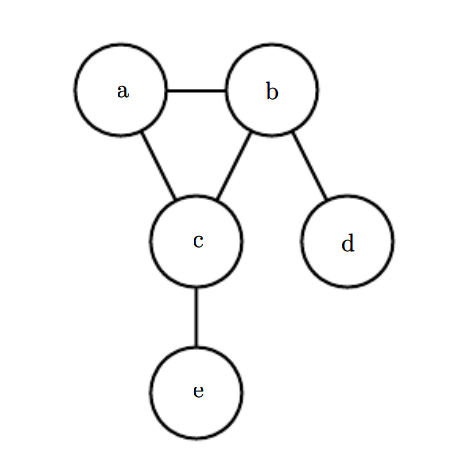
\includegraphics[height=0.3\textheight]{figures/undirected_graph_model}
    \caption{无向图模型实例}\label{fig:undirected_graph_model}
\end{figure}
无向图模型中的边为无向边。
无向图中任意两个节点都直接相连的部分为一个团{$\mathcal{C}^{(i)}$},
每一个团都可定义一个相关方程{$\phi^{(i)}(\mathcal{C}^{(i)})$}。
可以由归一化后的团相关方程来表示无向图模型的联合概率分布,
即:
\begin{equation}
    \label{eq:undirected_graph_model}
    p(\bm{x})=\frac{1}{Z}\prod_{i} \phi^{(i)} ( \mathcal{C}^{(i)} )
\end{equation}

图{\ref{fig:undirected_graph_model}}中,
{$a,b,c,d,e$}为随机变量。
该有向图模型的联合概率分布为:
\begin{equation}
    p(a,b,c,d,e)
    =\frac{1}{Z} \phi^{(1)}(a,b,c) \phi^{(2)}(b,d) \phi^{(3)}(c,e)
\end{equation}








% \subsection{注意力机制}

\end{document}